\chapter{The VFS Layer}\label{vfs}

% make sure to cover Ramfs operations - generic_file_splice_read, iter_file_splice_write and all sorts of goodies
% quotas implementation
% splicing in general - Splicing allows the user space to transfer data between two in-kernel memory buffers without copying the data to user space. This is useful, for example, for stackable file systems that pass data directly to the underlying file system.

Now that we've covered the main kernel structures related to file and filesystem access, highlighted the system call interface and the major subsystems that surround file access, this section will go into more detail about how the system call handlers above the VFS layer work, the internals of the VFS as well as major subsystems such as the dcache, buffer, page and inode caches. It will also cover the VFS to filesystem layer where the kernel calls into individual filesystems.

This chapter will dip much deeper into the kernel operations for filesystem support covering everything from file lookup to file creation to how I/O and the page cache operates. There will be several examples of using \cf{gdb} to analyze kernel structures to help.

%%%%%%%%%%%%%%%%%%%%%%%%%%%%%%%%%%%%%%%%%%%%%%%%%%%%%%%%%%%%%%%

\section{The VFS Entry Point}

Section \ref{syscalls} showed where in the kernel the source code can be found for the various Linux system call handlers. A lot of work performed at this layer includes marshaling system call arguments, calling common functions that can handle similar system calls, for example \cf{open(2)} and \cf{openat(2)}, and then calling into the \textit{Virtual File System} (VFS) interface. Figure \ref{fig:vfs-functions} shows where these functions reside with respect to other parts of the kernel.

\begin{figure}[h]
	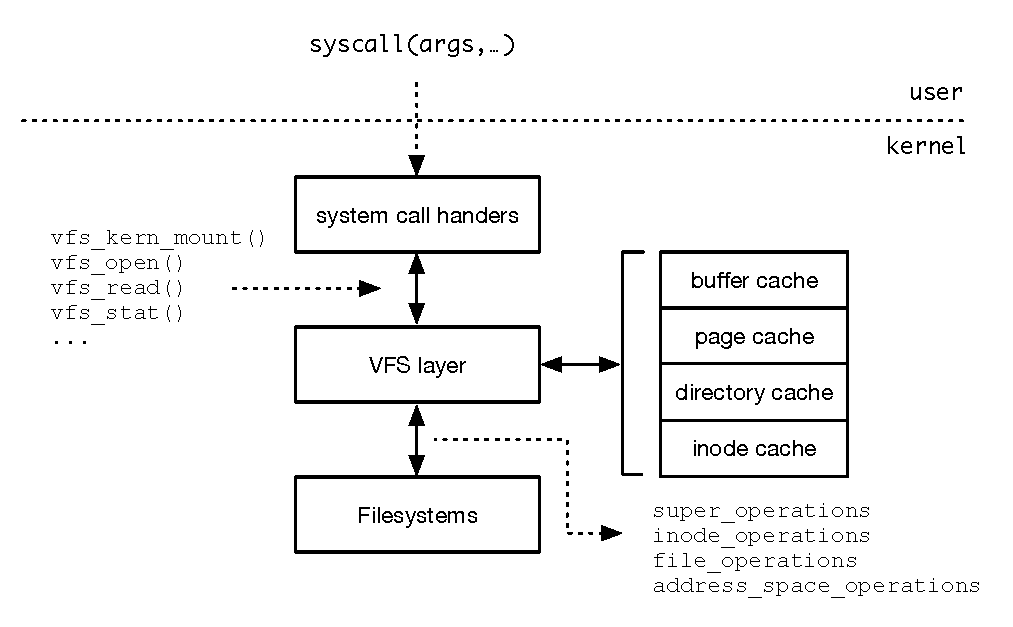
\includegraphics[scale=0.6]{figures/vfs-functions.pdf}
	\centering
	\caption{The Linux VFS Interface}
	\label{fig:vfs-functions}
\end{figure}

There are 56 VFS functions, split across 17 files, and all can be found in the \cf{fs} directory. In most cases, there is a function starting with \cf{vfs\_} which matches, or closely matches, the system call of the same name. Here are a few examples:

\begin{lstlisting}
init.c:       vfs_getattr(&path, stat, STATX_BASIC_STATS,
init.c:       vfs_mknod(mnt_user_ns(path.mnt), ...
namei.c:      vfs_open(&path, file);
namei.c:      vfs_create(mnt_userns, ...
namei.c:      vfs_rmdir(mnt_userns, ...
read_write.c: vfs_read(f.file, buf, count, ppos);
read_write.c: vfs_write(f.file, buf, count, ppos);
\end{lstlisting}

\noindent
The main structures handled in the VFS layer are \cf{file}, \cf{dentry} and \cf{inode} structures as described in the previous chapter. You may see some figures in Linux kernel documentation that differ slightly from this figure, specifically having the system call layer as part of the VFS layer but I think it's cleaner to keep the two layers separate. Note that this also differs from the original Sun/SVR4 VFS layer which generally pointed to the division between filesystem independent and filesystem dependent code at both the top layer of the kernel and at the filesystem later. Either way, it's important to recognize that there are two distinct interfaces, one entering filesystem independent code as part of system call handling or file access from other areas in the kernel and one where individual filesystems are called. Of course, in addition to calling individual filesystems, the VFS layer also calls into other subsystems such as those managing the directory, inode, buffer and page caches.

%%%%%%%%%%%%%%%%%%%%%%%%%%%%%%%%%%%%%%%%%%%%%%%%%%%%%%%%%%%%%%%

\section{VFS to Filesystem Interfaces}

There are four structures of operations that the kernel uses to call through to the underlying filesystem. There are almost 100 functions altogether across the four structures and each filesystem supports a subset of these functions. For example, SPFS only supports 35 operations and makes uses of generic kernel functions in some circumstances. Some of the more feature rich filesystems, or those who want more control over specific operations, will provide more fine-grain functions and be called more often. As an example, XFS provides closer to 100 different functions that the kernel can call.

Here are the operation structures are provided by each filesystem. For details about the functions in each structure, refer to section \ref{vfs-operations}. 

\begin{itemize}
	\item \cf{super\_operations} -- a set of functions that operate at the filesystem level including functions to get 
		filesystem statistics, sync the filesystem and several inode-related operations (allocating, writing, freeing, etc).
		Note that the filesystem function to be called during mount processing is provided to the kernel when the 
		filesystem registers itself.
	\item \cf{inode\_operations} -- filesystems will likely define three different sets of inode operations which
		will be attached to directory inodes, regular file inodes and symlink inodes. Each exports a different set of operations.
	\item \cf{file\_operations} -- these functions are attached to the \cf{f\_op} field of the file structure and include
		operations such as read, write and lseek.
	\item \cf{address\_space\_operations} -- attached to \cf{inode->i\_mapping->a\_ops} by the filesystem, these 
		functions provide interaction between the filesystem and the Linux page cache. Generally speaking, file
		I/O will utilize these functions. \textbf{(XXX---see read/write in file operations - what's the difference?}
\end{itemize}

\noindent
Which operations to provide is dependent on the type of file. Using SPFS as an example, here are the operations attached for directory files, regular files and symlinks:

\begin{lstlisting}
sp_dir.c:    inode->i_op = &sp_file_inops;
sp_dir.c:    inode->i_op = &sp_dir_inops;
sp_dir.c:    inode->i_op = &sp_symlink_operations;
\end{lstlisting}

\noindent
Looking at directory and symlink operations, you can see operations that are some operations that are directory specific and some that are symlink specific:

\begin{lstlisting}
struct inode_operations sp_dir_inops = {
    .create     = sp_create,
    .lookup     = sp_lookup,
    .mkdir      = sp_mkdir,
    .rmdir      = sp_rmdir,
    .link       = sp_link,
    .unlink     = sp_unlink,
    .symlink    = sp_symlink,
    .rename     = sp_rename
};   

static const struct inode_operations sp_symlink_operations = {
    .readlink   = sp_readlink,
    .get_link   = sp_page_get_link,
    .getattr    = sp_getattr, 
};  
\end{lstlisting}

\noindent
The SPFS operations vectors will be described in chapter \ref{disk-fs}. For the filesystems in the Linux source tree, search the directory for a specific filesystem to see what vectors it provides. For example:

\begin{lstlisting}
$ [*\bfseries pwd*]
/Users/spate/src/linux-6.3.3/fs/xfs
$ [*\bfseries grep inode\_operations *.c*]
xfs_iops.c:static const struct inode_operations \
                xfs_inode_operations = {
xfs_iops.c:static const struct inode_operations \
                xfs_dir_inode_operations = {
xfs_iops.c:static const struct inode_operations \
                xfs_dir_ci_inode_operations = {
xfs_iops.c:static const struct inode_operations \
                xfs_symlink_inode_operations = {
xfs_iops.c:    inode->i_op = &xfs_inode_operations;
xfs_iops.c:    inode->i_op = &xfs_dir_ci_inode_operations;
xfs_iops.c:    inode->i_op = &xfs_dir_inode_operations;
xfs_iops.c:    inode->i_op = &xfs_symlink_inode_operations;
xfs_iops.c:    inode->i_op = &xfs_inode_operations;
\end{lstlisting}

%%%%%%%%%%%%%%%%%%%%%%%%%%%%%%%%%%%%%%%%%%%%%%%%%%%%%%%%%%%%%%%

\section{Registering Filesystems}\label{register-fs}

Individual filesystems are registered and unregistered with the Linux kernel by calling the \cf{register\_filesystem()} and \cf{unregister\_filesystem()} functions. You will see calls to register filesystems from many places in the kernel source, not just from within the \cf{fs} directory and individual filesystems under \cf{fs}. These calls are made when a filesystem module is being loaded or unloaded.

\begin{table}[h]
\begin{tabular}{ll}
\parbox[l]{0.6in}{
\includegraphics[scale=0.8]{figures/src-xref.pdf}} & \parbox[l]{4in}{\small{\cf{fs/filesystems.c} contains various functions for managing the list of registered filesystems together with code for displaying these filesystems through the \cf{/proc/filesystems} interface.}}
\end{tabular}
\end{table}

\noindent
The code for \cf{register\_filesystem()} is actually quite simple with the main parts of the function shown below:

\begin{lstlisting}
int
[*\bfseries register\_filesystem*](struct file_system_type * fs)
{
    int res = 0;
    struct file_system_type **p;

    [*\bfseries write\_lock*](&file_systems_lock);
    p = [*\bfseries find\_filesystem*](fs->name, strlen(fs->name));
    if (*p)
        res = -EBUSY;
    else
        *p = fs;
    [*\bfseries write\_unlock*](&file_systems_lock);
    return res;
}
\end{lstlisting}

\noindent
Using SPFS as an example, here is the \cf{file\_system\_type} structure that is passed as an argument to \cf{register\_filesystem()}:

\begin{lstlisting}
static struct file_system_type spfs_fs_type = {
    .owner      = THIS_MODULE,
    .name       = "spfs",
    .mount      = spfs_mount,
    .kill_sb    = kill_block_super,
    .fs_flags   = FS_REQUIRES_DEV,
};
\end{lstlisting}

\noindent
The call to \cf{find\_filesystem()} is also straightforward. It walks through the linked list of current registered filesystems comparing their names against the name specified by the filesystem being registered. 

\begin{lstlisting}
static struct file_system_type **
[*\bfseries find\_filesystem*](const char *name, unsigned len)
{
    struct file_system_type **p;
    for (p = &file_systems; *p; p = &(*p)->next)
        if (strncmp((*p)->name, name, len) == 0 &&
            !(*p)->name[len])
            break;
    return p;
}
\end{lstlisting}

\noindent
On return from \cf{register\_filesystem()}, if a match was found, the filesystem has already been registered and an error is returned. If it had not been registered previously, the filesystem is simply added to the end of the linked list and can now be mounted. Note that the \cf{file\_systems\_lock} must be taken since this action could be performed in parallel by two different processes.

%---------------------------------------------------------------------------------------------------------------------------------------------------------------------

\subsection{Unregistering Filesystems}

Filesystems are unregistered by a user calling the \cf{rmmod(8)} command. The code for unregistering a filesystem is straightforward and involves walking the list of registered filesystems to see if the filesystem is registered. 

\begin{lstlisting}
int 
[*\bfseries unregister\_filesystem*](struct file_system_type * fs)
{
    struct file_system_type **tmp;

    [*\bfseries write\_lock*](&file_systems_lock);
    tmp = &file_systems;
    while (*tmp) {
        if (fs == *tmp) {
            *tmp = fs->next;
            fs->next = NULL;
            [*\bfseries write\_unlock*](&file_systems_lock);
            [*\bfseries synchronize\_rcu*]();
            return 0;
        }
        tmp = &(*tmp)->next;
    }
    [*\bfseries write\_unlock*](&file_systems_lock);
    return -EINVAL;
}
\end{lstlisting}

\noindent
If the filesystem is found on the list, it will be removed by setting the \cf{next} field of the previous structure to point to the filesystem referenced by the \cf{next} field of the filesystem that the kernel is removing.

You will notice that there is no check to see if there are any filesystems of this type that are currently mounted before the \cf{file\_system\_type} structure is removed from the list of registered filesystems. This check is made during module unload (\cf{rmmod(8)}) time before the module exit function is called. 

\begin{table}[h]
\begin{tabular}{ll}
\parbox[l]{0.6in}{
\includegraphics[scale=0.8]{figures/src-xref.pdf}} & \parbox[l]{4in}{\small{Module removal code can be found in \cf{module/main.c}. Start with the function \cf{delete\_module()}}}
\end{tabular}
\end{table}

%------------------------------------------------------------------------------------------------------------------------------------------------------------

\subsection{KGDB --- Analyzing the List of Registered Filesystems}

The list of registered filesystems is a simple linked list with the head of the list referenced by the global variable \cf{file\_systems}. Each element of the list is of type "\cf{struct file\_system\_type}" which has a field \cf{next} which points to the next filesystem in the list. In \cf{gdb}, to print the first several entries, simply start at \cf{file\_systems} and keep using the \cf{next} field to advance through the list

\begin{lstlisting}
(gdb) [*\bfseries pipe p *file\_systems | grep 'name ='*]
  name = 0xffff8000098b4960 "sysfs",
(gdb) [*\bfseries pipe p *file\_systems->next | grep 'name ='*]
  name = 0xffff8000097fcbb0 "tmpfs",
(gdb) [*\bfseries pipe p *file\_systems->next->next | grep 'name ='*]
  name = 0xffff80000984b608 "bdev",
(gdb) [*\bfseries pipe p *file\_systems->next->next->next | grep 'name ='*]
  name = 0xffff80000984c210 "proc",
\end{lstlisting}

\noindent
Walking through this list by hand is similar to what happens when you look into the contents of \cf{/proc/filesystems} as follows:

\begin{lstlisting}
$ [*\bfseries cat /proc/filesystems*]
nodev	sysfs
nodev	tmpfs
nodev	bdev
nodev	proc
...
\end{lstlisting}

\noindent
The \cf{filesystems\_proc\_show()} function in \cf{fs/filesystems.c} walks through the list and displays each filesystem and whether it requires a physical device or not.

\begin{lstlisting}
static int 
[*\bfseries filesystems\_proc\_show*](struct seq_file *m, void *v)
{
    struct file_system_type * tmp;

    [*\bfseries read\_lock*](&file_systems_lock);
    tmp = file_systems;
    while (tmp) {
        [*\bfseries seq\_printf*](m, "%s\t%s\n",
            (tmp->fs_flags & FS_REQUIRES_DEV) ? "" : "nodev",
            tmp->name);
        tmp = tmp->next;
    }
    [*\bfseries read\_unlock*](&file_systems_lock);
    return 0;
}
\end{lstlisting}

\noindent
As with the other functions shown in this section, \cf{filesystems\_proc\_show()} starts with the global variable \cf{file\_systems}, walks through the list and prints the name of the filesystem (\cf{tmp->name}) together with \cf{nodev} if it's a pseudo filesystem.

%%%%%%%%%%%%%%%%%%%%%%%%%%%%%%%%%%%%%%%%%%%%%%%%%%%%%%%%%%%%%

\section{Mounting and Unmounting Filesystems}

Section \ref{struct-mount} described the \cf{file\_system\_type} and \cf{super\_block} structures which are used during mounting of filesystems and to manage the list of mounted filesystems. Here we describe how the VFS mounts a filesystem and utilizes these structures.

At the time of writing, Linux filesystems are mounted using one of two different mechanisms. The first path, now called \textit{legacy mounts} has been around for many years with a few minor changes here and there. The new form which utilizes 
a \textit{filesystem context} structure into which is placed:

\begin{itemize}
	\item Filesystem type.
	\item Namespaces.
	\item Source/Device names (there may be multiple).
	\item Superblock flags (SB\_*).
	\item Security details.
	\item Filesystem-specific data, as set by the mount options.
\end{itemize}

\noindent
This structure is passed ... XXX

At the time of writing, some filesystems have been switched over to the new method of mounting while several are still using the legacy method. As an example, as of September 2023, btrfs has changes made to support the new method but the path has not yet been applied to the mainline Linux kernel sources. Both methods will be described in this section.

% https://stackoverflow.com/questions/62499748/how-does-do-new-mount-fc-mount-real-file-systems-like-ext4 - overview

The new style mount method is described in the following document:

\begin{table}[h]
\begin{tabular}{lcl}
\parbox[r]{0.5in}{
\includegraphics[scale=0.15]{figures/url.png}} & \parbox[l]{0.55in}{URL \arabic{urls}} & \parbox[l]{3in}{\cf{https://tinyurl.com/ykpvxfkx}}
\end{tabular}
\end{table}
\stepcounter{urls}
% https://www.kernel.org/doc/Documentation/filesystems/mount_api.txt - kernel mount API

\noindent
but the rationale for why it was introduced is not well documented XXX

This section will start by showing the interaction between the VFS layer at the filesystem which is where the main differences apply between the two styles of mounting. The code through the VFS layer should then become clearer and will be described later in this section.

%------------------------------------------------------------------------------------------------------------------------------------------------------------

\subsection{Legacy Mounts}

The legacy mount process is described in this section and was what I originally implemented in SPFS using the 6.3.3 kernel. I then switched to using the filesystem context method but rather than throw away the legacy code, I'm documenting it here since the process is still used by many of the existing filesystems.

When I wrote my last book (\cite{pate-filesystems}), 20 years ago, Linux filesystems were still declared by making a call to \cf{register\_filesystem()} as follows:

\begin{lstlisting}
static [*\bfseries DECALRE\_FSTYPE\_DEV*](uxfs_fs_type, "uxfs", ux_read_super);

static int [*\bfseries \_\_init\_uxfs\_fs*](void)
{
    return [*\bfseries register\_filesystem*](&uxfs_fs_type);
}
\end{lstlisting}

\noindent
Only one function was provided and that function was called to read in the filesystem's superblock after the kernel had already created the corresponding \cf{super\_block} structure.

The process is still very similar today for legacy mounts. The filesystem will create a \cf{file\_system\_type} structure in which it places information about the filesystem. 

\begin{lstlisting}
static struct file_system_type spfs_fs_type = {
    .owner      = THIS_MODULE,
    .name       = "spfs",   
    .mount      = spfs_mount,
    .kill_sb    = kill_block_super,
    .fs_flags   = FS_REQUIRES_DEV,
};  
\end{lstlisting}

\noindent
When a filesystem module is loaded, it passes a pointer to this structure through a call to \cf{register\_filesystem()}. One of the elements of the structure is a \textit{mount} function which is called by the kernel each time a filesystem of this type is mounted. For SPFS, the filesystem that will be described in chapter \ref{disk-fs}, these functions and structures are shown in figure \ref{fig:super-operations}.

\begin{figure}[h]
	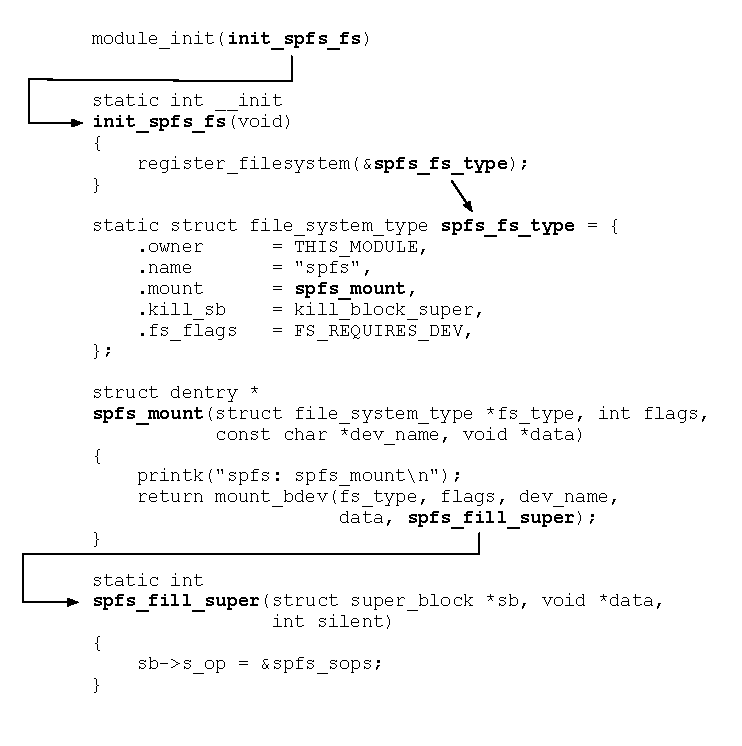
\includegraphics[scale=0.8]{figures/super_operations.pdf}
	\centering
	\caption{Mounting a Filesystem Using Legacy Mount Mode}
	\label{fig:super-operations}
\end{figure}

In the same structure, the filesystem may specify a function to be called when the filesystem is being unmounted. \textbf{Need to better understand all the places at which it's called}.

The code for \cf{spfs\_mount()} is very simple, relying solely on a call to \cf{mount\_bdev()}. It passes \cf{spfs\_fill\_super()} as as argument.

\begin{lstlisting}
static struct dentry *
[*\bfseries spfs\_mount*](struct file_system_type *fs_type, int flags, 
			   const char *dev_name, void *data)
{
    return [*\bfseries mount\_bdev*](fs_type, flags, dev_name, data, 
                      [*\bfseries spfs\_fill\_super*]);
}
\end{lstlisting}

\noindent
The role of \cf{sp\_fill\_super()} is to:

\begin{itemize}
	\item Allocate filesystem-specific data structures to be used in-core.
	\item Read the filesystem superblock from disk.
	\item Read in the root inode and instantiate it in the dcache.
	\item Set the \cf{s\_op} field of the \cf{super\_block} structure to reference a vector of filesystem operations. These
		typically involve inode-related operations such as allocating, freeing, writing and eviction.
\end{itemize}

\noindent
As the book progresses and has been out for some time, I suspect that most filesystems will move away from legacy mounts. To find those that still use legacy mounts, run the following inside the \cf{fs} directory:

\begin{lstlisting}
$ [*\bfseries grep '\textbackslash.mount' */*.c*]
9p/vfs_super.c:	.mount = v9fs_mount,
adfs/super.c:	.mount		= adfs_mount,
affs/super.c:	.mount		= affs_mount,
autofs/init.c:	.mount		= autofs_mount,
befs/linuxvfs.c:	.mount		= befs_mount,
bfs/inode.c:	.mount		= bfs_mount,
btrfs/super.c:	.mount		= btrfs_mount,
...
\end{lstlisting}

%------------------------------------------------------------------------------------------------------------------------------------------------------------

\subsection{Mounting Using Filesystem Context}

It looks like get\_tree() is the new version of spfs\_mount() / spfs\_fill\_super() (perhaps)

xxxx

As described in Documentation/filesystems/mount\_api.rst the new process consists of the following steps:

\begin{enumerate}
	\item Create a filesystem context.
	\item Parse the parameters and attach them to the context.  Parameters are expected to be passed individually 
		from user-space, though legacy binary parameters can also be handled.
	\item Validate and pre-process the context.
	\item Get or create a superblock and mountable root.
	\item Perform the mount.
	\item Return an error message attached to the context.
	\item Destroy the context.
\end{enumerate}

Don't know if this is the right order yet ... see Documentation/filesystems/mount\_api.rst for more info

\begin{lstlisting}
struct [*\bfseries file\_system\_type*] {
    int (*[*\bfseries init\_fs\_context*])(struct fs_context *);
    const [*\bfseries struct fs\_parameter\_spec*] *parameters;
    ...
    struct dentry *(*[*\bfseries mount*]) (struct file_system_type *, int,
               const char *, void *);
    void (*[*\bfseries kill\_sb*]) (struct super_block *);
    ...
}
\end{lstlisting}

There is an \cf{fs\_context} structure that is used during mount processing. It's mentioned all over the place in the fs directory. There is also a file \cf{fs/fs\_context.c}.

\begin{lstlisting}
struct fs_context {
    const struct fs_context_operations *ops;
    struct file_system_type            *fs_type;
    void                               *fs_private;
    struct dentry                      *root;
    struct user_namespace              *user_ns;
    struct net                         *net_ns;
    const struct cred                  *cred;
    char                               *source;
    char                               *subtype;
    void                               *security;
    void                               *s_fs_info;
    unsigned int                        sb_flags;
    unsigned int                        sb_flags_mask;
    unsigned int                        s_iflags;
    unsigned int                        lsm_flags;
    enum fs_context_purpose             purpose:8;
    ... 
};
\end{lstlisting}

\noindent
XXX a bunch of filesystems deal with this struct. SPFS does not. take fs/ramfs as an example .. 

\begin{lstlisting}
static struct file_system_type ramfs_fs_type = {
    .name             = "ramfs",
    .init_fs_context  = [*\bfseries ramfs\_init\_fs\_context*],
    .parameters       = ramfs_fs_parameters,
    .kill_sb          = ramfs_kill_sb,
    .fs_flags         = FS_USERNS_MOUNT,
};

struct ramfs_fs_info {
    struct ramfs_mount_opts mount_opts;
}; 

int 
[*\bfseries ramfs\_init\_fs\_context*](struct fs_context *fc)
{
    struct ramfs_fs_info *fsi;

    fsi = kzalloc(sizeof(*fsi), GFP_KERNEL);

    fsi->mount_opts.mode = RAMFS_DEFAULT_MODE;
    fc->s_fs_info = fsi;
    fc->ops = &ramfs_context_ops;
    return 0;
}
\end{lstlisting}

\noindent
only seems to be one argument and that's stuffed in a struct referenced from the private super\_block pointer (s\_fs\_info) - if you look at ext4, the usage is much more extensive. Note that (s\_fs\_info) is listed as FS private data but search for it in fs/* and there are references to something else. Double check on this. my usage is the same as BFS and likely others. Hmm!

%------------------------------------------------------------------------------------------------------------------------------------------------------------------------

\subsection{Mounting Filesystems at the VFS Layer}

Figure \ref{fig:super-operations} shows how a filesystem module establishes itself with the kernel during module load time. It also covered how the filesystem registers its \cf{file\_system\_type} structure which is then held on the linked list of available filesystems accessible through global variable \cf{file\_systems}. Together with the "mount" function provided and the \cf{fs\_flags} field (which will be set to \cf{FS\_REQUIRE\_DEV} if a block device is needed to host this filesystem, this provides enough for the kernel to be able to perform a mount operation when requested for this filesystem type.

\begin{table}[h]
\begin{tabular}{ll}
\parbox[l]{0.6in}{
\includegraphics[scale=0.8]{figures/src-xref.pdf}} & \parbox[l]{4in}{\small{Look for "\cf{SYSCALL\_DEFINE5(mount}"} in \cf{fs/namespace.c} for the starting point for handling the \cf{mount(2)} system call.}
\end{tabular}
\end{table}

\noindent
The system call handler for mounting a filesystem starts by copying in the type of the filesystem, the device name and any mount options before issuing a call to \cf{do\_mount()}.

\begin{lstlisting}
SYSCALL_DEFINE5([*\bfseries mount*], char __user *, dev_name, char __user *, 
                dir_name, char __user *, type, unsigned long, 
                flags, void __user *, data)
{
    char *kernel_type;
    char *kernel_dev;
    void *options;

    kernel_type = [*\bfseries copy\_mount\_string*](type);
    kernel_dev = [*\bfseries copy\_mount\_string*](dev_name);
    options = [*\bfseries copy\_mount\_options*](data);
    ret = [*\bfseries do\_mount*](kernel_dev, dir_name, kernel_type, 
                   flags, options);
}
\end{lstlisting}

\noindent
The \cf{do\_mount()} function needs to resolve the mount point passed to \cf{mount(2)} to a directory inode before the filesystem can be mounted. The copying of the pathname is done with a call to \cf{user\_path\_at()}. The \cf{path\_put()} function calls \cf{dput()} releases it's hold on the dentry held in the \cf{path} structure before calling \cf{mnt\_put} which calls \cf{mntput\_no\_expire()} -- \textbf{XXX -- which look complicated -- come back}.

\begin{lstlisting}
long 
[*\bfseries do\_mount*](const char *dev_name, const char __user *dir_name,
         const char *type_page, unsigned long flags, 
         void *data_page)
{
    struct path path;

    [*\bfseries user\_path\_at*](AT_FDCWD, dir_name, LOOKUP_FOLLOW, &path);
    ret = [*\bfseries path\_mount*](dev_name, &path, type_page, flags, 
                     data_page);
    [*\bfseries path\_put*](&path);
    return ret;
}
\end{lstlisting}

\noindent
The functions called by \cf{user\_path\_at()} are:

\small
\vspace{10pt}
\noindent
\cf{user\_path\_at()} $\rightarrow$ \cf{user\_path\_at\_empty()} $\rightarrow$ \cf{filename\_lookup()} $\rightarrow$

\vspace{1pt}
\cf{path\_lookupat()}$\rightarrow$ \cf{link\_path\_walk()}

\vspace{10pt}
\normalsize
\noindent
Section \ref{openfile} covers Linux kernel pathname resolution in detail and specifically covers the function \cf{link\_path\_walk()} and functions calling it.

\textbf{Back to mounting - need to expand \cf{do\_mount()}}

\cf{do\_new\_mount\_fc()} is the function called once everything is set up (fs context etc) and is the one that allocates a new \cf{vfsmount} structure. 

Here are the \cf{mount} and \cf{vfsmount} structures. Note that \cf{vfsmount} is embedded within the \cf{mount} structure.

\begin{lstlisting}
struct [*\bfseries vfsmount*] {
    struct dentry         *mnt_root;  /* root of mounted tree */
    struct super_block    *mnt_sb;    /* ptr to superblock */
    int                    mnt_flags;  
    struct user_namespace *mnt_userns;
}

struct [*\bfseries mount*] {
    struct hlist_node     mnt_hash;
    struct mount         *mnt_parent;
    struct dentry        *mnt_mountpoint;
    struct [*\bfseries vfsmount*]       mnt;
    ....
    struct mnt_namespace *mnt_ns;    /* containing namespace */
    struct mountpoint    *mnt_mp;    /* where is it mounted */
}
\end{lstlisting}

\noindent
The \cf{super\_block} structure has a field that contains a list of mounts for this filesystem/device since a filesystem (one the one block device) can be mounted in multiple places at the same time. The comment in the source code specifies that this field should not be accessed by filesystems.

\begin{lstlisting}
struct list_head s_mounts; 
\end{lstlisting}

\noindent
Figure  \ref{fig:mount-vfsmount} shows how these structures are linked together following a call to mount a filesystem. If this is the last mount, we can locate its structures from the \cf{prev} of the \cf{super\_blocks} list head.

\begin{figure}[h]
	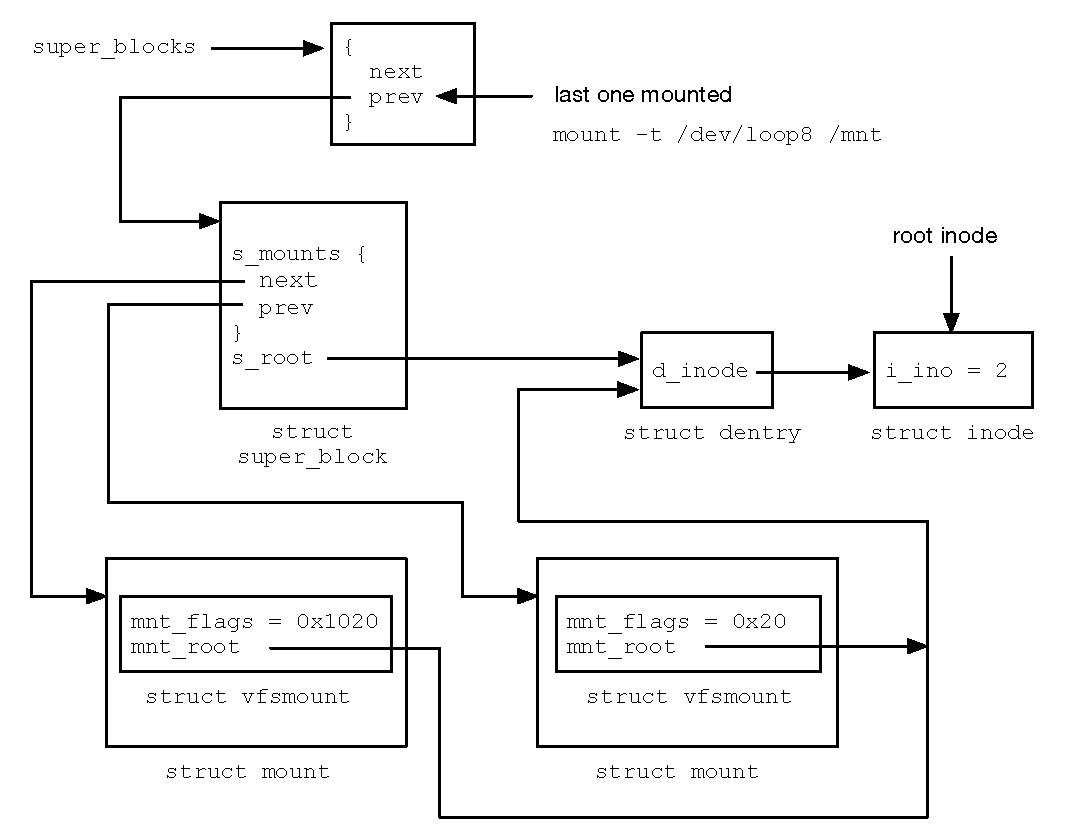
\includegraphics[scale=0.6]{figures/mount-vfsmount.pdf}
	\centering
	\caption{Structures for the last mounted filesystem}
	\label{fig:mount-vfsmount}
\end{figure}

For the \cf{mnt\_flags} field here are the values for each of the \cf{mount} structures:

\begin{lstlisting}
#define MNT_RELATIME	0x20
#define MNT_SHARED	0x1000
\end{lstlisting}

\noindent
\textbf{XXX -- not sure why at this point we have two mount structures, perhaps something to do with namespaces?}

\textbf{There is also \cf{struct mountpoint} - what the hell is that???}

\begin{lstlisting}
struct mountpoint {
    struct hlist_node  m_hash;
    struct dentry     *m_dentry;
    struct hlist_head  m_list;
    int                m_count;
};
\end{lstlisting}

\noindent
The following function allocates a new \cf{mountpoint} structure as follows:

\begin{lstlisting}
static struct mountpoint *
[*\bfseries get\_mountpoint*](struct dentry *dentry)
{
    ...
    new = kmalloc(sizeof(struct mountpoint), GFP_KERNEL);
\end{lstlisting}

\noindent
This is called indirectly from \cf{do\_add\_mount()} as well as other places.

references

% https://stackoverflow.com/questions/57361052/why-does-mount-structure-has-two-mountpoint-fields

%------------------------------------------------------------------------------------------------------------------------------------------------------------------------

\subsection{KGDB -- A Look at Structures Following Mount}

This section will explore what happens following a call to \cf{mount(1)} to mount a filesystem as follows:

\begin{lstlisting}
$ [*\bfseries sudo mount -t spfs /dev/loop8 /mnt*]
\end{lstlisting}

\noindent
It's easy to find the corresponding \cf{super\_block} structure associated with this mount by using one of the Linux Python helper functions as follows:

\begin{lstlisting}
(gdb) [*\bfseries lx-mounts*]
mount            super_block      devname    path fstype options
...
0xf...812f3ea500 0xf...8127b7c800 /dev/loop8 /mnt spfs   rw,r...
\end{lstlisting}

\noindent
The second address is the address of the \cf{super\_block} structure and the first address is the associated \cf{mount} structure for this mount point. We can also get the same information as follows:
\begin{lstlisting}
(gdb) [*\bfseries p super\_blocks*]
$4 = {
  next = 0xffff88810005a800,
  prev = 0xffff888127b7c800 
}
\end{lstlisting}

\noindent
Recall that the list of \cf{super\_block} structures for all mounted filesystems can be accessed through the global variable \cf{super\_blocks}. What is shown here are pointers to the first and last elements of the list. In this example, the "spfs" filesystem is  the last one mounted. This is saved as a convenience variable and the \cf{s\_mounts} field is displayed:

\begin{lstlisting}
(gdb) [*\bfseries set \$sb = (struct super\_block *)0xffff888127b7c800*]
(gdb) [*\bfseries p \$sb->s\_mounts*]
$3 = {
  next = 0xffff88812f3ea578,
  prev = 0xffff888101952cf8
}
\end{lstlisting}

\noindent
The filesystem has only been mounted once so why are there two entries? Let's explore further. The \cf{mount} structures are linked together through the \cf{mnt\_instance} field which is 0x78 bytes into the \cf{mount} structure. Take the first address displayed above. We can confirm this offset as follows:

\begin{lstlisting}
(gdb) [*\bfseries p \&\$mount->mnt\_instance*]
$39 = (struct list_head *) 0xffff88812f3ea578
\end{lstlisting}

\noindent
If we print out each one, both display \cf{mnt} and \cf{/dev/loop8} adding to the confusion:

\begin{lstlisting}
(gdb) [*\bfseries set \$m1 = (struct mount *)0xffff88812f3ea500*]    # - 0x78
(gdb) [*\bfseries set \$m2 = (struct mount *)0xffff888101952c80*]    # - 0x78
(gdb) [*\bfseries p \$m1->mnt\_mountpoint->d\_name.name*]
$49 = (const unsigned char *) 0xffff88812f8324b8 "mnt"
(gdb) [*\bfseries p \$m1->mnt\_devname*]
$46 = 0xffff8881008d4b10 "/dev/loop8"
(gdb) [*\bfseries p \$m2->mnt\_mountpoint->d\_name.name*]
$47 = (const unsigned char *) 0xffff88812f8324b8 "mnt"
(gdb) [*\bfseries p \$m2->mnt\_devname*]
$48 = 0xffff8881008d4230 "/dev/loop8"
\end{lstlisting}

\noindent
One thing that is different is the \cf{mnt\_flags} field:

\begin{lstlisting}
(gdb) [*\bfseries p/x \$m1->mnt.mnt\_flags*]
$27 = 0x1020
(gdb) [*\bfseries p/x \$m2->mnt.mnt\_flags*]
$28 = 0x20
\end{lstlisting}

\noindent
As described above, they have the following values:

\begin{lstlisting}
#define MNT_RELATIME	0x20
#define MNT_SHARED	0x1000
\end{lstlisting}

\noindent
\textbf{That's all well and good but what exactly does it mean?}

%------------------------------------------------------------------------------------------------------------------------------------------------------------------------

\subsection{Unmounting Filesystems}

Unmounting a filesystem starts with the \cf{umount(8)} command and/or the \cf{umount(2)} / \cf{umount2(2)} system calls.

\begin{table}[h]
\begin{tabular}{ll}
\parbox[l]{0.6in}{
\includegraphics[scale=0.8]{figures/src-xref.pdf}} & \parbox[l]{4in}{\small{Source code for handling unmounting of filesystems can be found in \cf{fs/namespace.c} and \cf{fs/super.c} AND XXX}}
\end{tabular}
\end{table}

\noindent
The entry point in the kernel is \cf{ksys\_umount()} which has two calls as follows:

\begin{lstlisting}
static int 
[*\bfseries ksys\_umount*](char __user *name, int flags)
{
    struct path path;

    // basic validity checks on "flags" done first

    ret = [*\bfseries user\_path\_at*](AT_FDCWD, name, lookup_flags, &path);
    return [*\bfseries path\_umount*](&path, flags);
}
\end{lstlisting}

\noindent
The first call to \cf{user\_path\_at} is responsible for looking up the mount point specified in the call to \cf{umount(2)}. This function calls \cf{filename\_lookup()} to resolve the pathname which in turn calls \cf{path\_lookupat()} which is described in section \cf{pathname-set}.

The \cf{path} structure contains a dentry for the directory looked up and the \cf{vfsmount} for the filesystem on which is found.

\begin{lstlisting}
int
[*\bfseries path\_umount*](struct path *path, int flags)
{
    struct mount *mnt = real_mount(path->mnt);
    int ret;

    ret = [*\bfseries can\_umount*](path, flags);
    if (!ret)
        ret = [*\bfseries do\_umount*](mnt, flags);

    dput(path->dentry);
    [*\bfseries mntput\_no\_expire*](mnt);
    return ret;
}
\end{lstlisting}

\noindent
There are several checks performed by \cf{can\_umount()} such as whether the caller has permission to unmount, that the path is the root of the mounted filesystem and \textbf{check\_mnt()????}

TBD

%%%%%%%%%%%%%%%%%%%%%%%%%%%%%%%%%%%%%%%%%%%%%%%%%%%%%%%%%%%%%%%

\section{Namespace Creation and Handling}

xxx

All of the namespaces are created using the \cf{clone(2)} or \cf{unshare(2)} system calls. XXX why so many entry points in the kernel??

\begin{table}[h]
\begin{tabular}{ll}
\parbox[l]{0.6in}{
\includegraphics[scale=0.8]{figures/src-xref.pdf}} & \parbox[l]{4in}{\small{The system call handler for the \cf{clone} system call cand be found in \cf{kernel/fork.c}. Look for the functions \cf{kernel\_clone()} and \c{ksys\_unshare()}}}
\end{tabular}
\end{table}

\noindent
XXX - the code looks horrendous! Not going to be easy to figure out.

clone -> \cf{kernel\_clone()}

unshare -> \cf{ksys\_unshare()}

%-----------------------------------------------------------------------------------------------------------------------------------------------------------------

\subsection{Handling \cf{chroot(2)}}

The \cf{chroot(2)} system call is very straightforward. Figure \ref{fig:chroot-fields} shows the \cf{fs} field of the \cf{task\_struct} pointing to an \cf{fs\_struct} structure which contains pointers to the root directory and the current working directory. All that the kernel needs to do for \cf{chroot(2)} is to ensure that the \cf{path} argument of the system call references a valid directory and that the process has permission to access it.

\begin{figure}[h]
	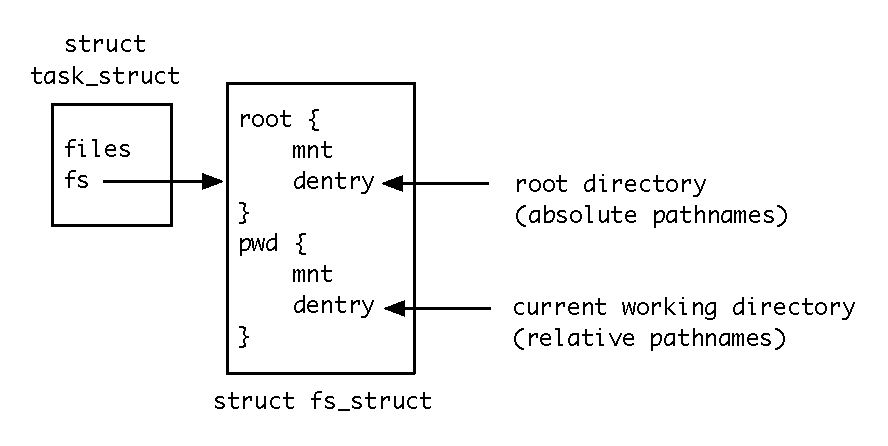
\includegraphics[scale=0.6]{figures/chroot-fields.pdf}
	\centering
	\caption{Switching a process's root directory with \cf{chroot(2)}}
	\label{fig:chroot-fields}
\end{figure}

\noindent
Here is the system call entry point for handling \cf{chroot(2)}:

\begin{lstlisting}
SYSCALL_DEFINE1([*\bfseries chroot*], const char __user *, filename)
{   
    struct path path;

retry:
    error = [*\bfseries user\_path\_at*](AT_FDCWD, filename, 
                         lookup_flags, &path);
    
    error = [*\bfseries path\_permission*](&path, MAY_EXEC | MAY_CHDIR);
    [*\bfseries set\_fs\_root*](current->fs, &path);
    error = 0;
    [*\bfseries path\_put*](&path);
    return error;
}
\end{lstlisting}

\noindent
Assuming the path is valid, \cf{set\_fs\_root()} is called to update the root directory and a hold on the previous root is dropped.

\begin{lstlisting}
void 
[*\bfseries set\_fs\_root*](struct fs_struct *fs, const struct path *path)
{
    struct path old_root;

    [*\bfseries path\_get*](path);
    spin_lock(&fs->lock);
    old_root = fs->root;
    fs->root = *path;
    spin_unlock(&fs->lock);
    if (old_root.dentry)
        [*\bfseries path\_put*](&old_root);
}
\end{lstlisting}

\noindent
At this point, any pathname resolution calls starting with "/" will start at this new root directory.

%-----------------------------------------------------------------------------------------------------------------------------------------------------------------

\section{KGDB -- Analyzing Mount Namespace Creation}

xxx

%%%%%%%%%%%%%%%%%%%%%%%%%%%%%%%%%%%%%%%%%%%%%%%%%%%%%%%%%%%%%%%

\section{Opening a File / Pathname Resolution}\label{openfile}

Figure \ref{fig:open-fd-alloc} shows the high-level paths followed for opening a file from \cf{do\_sys\_open()} through to \cf{path\_open\_at()} which calls for pathname resolution and opens the file. On a successful return from this function, the file has been found, it will have been opened and a \cf{file} structure is allocated and returned for it.

\begin{figure}[h]
	\centering
	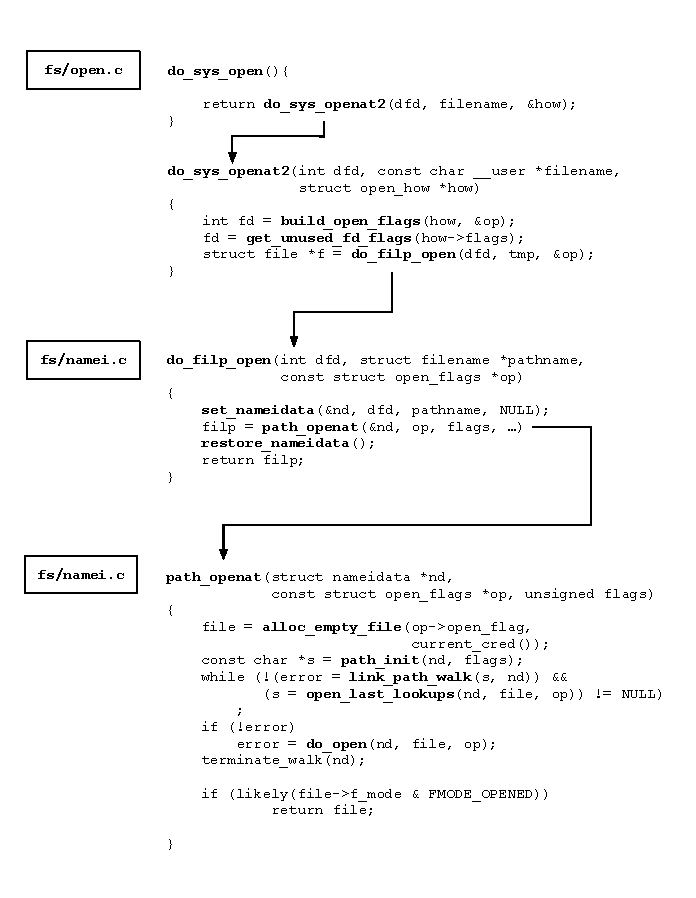
\includegraphics[scale=0.8]{figures/open-fd.pdf}
	\caption{Main Kernel Routines for Opening a File / Allocating a File Descriptor}
	\label{fig:open-fd-alloc}
\end{figure}

\noindent
 \cf{get\_unused\_fd\_flags()} could return very quickly if an available file descriptor is available. If not, the code gets quite complex in allocating new structures. This will be described in section \ref{fd-expand}. Either way, a call is made to \cf{do\_filp\_open()} which allocates a \cf{nameidata} structures that contains information needed to perform pathname resolution (\cf{link\_path\_walk()} on the pathname that has been passed to one of the open system call. This walks through the path one component at a time until the last component is reached. If everything is successful at this point, a call is made to \cf{do\_open()} to actually open the file.
 
 \textbf{XXX - finish this section and do fd / file expansion}
 
 \textbf{XXX - need to go back to previous chapter and see how open flags/mode map to f\_flags and f\_mode - around line 599}

%---------------------------------------------------------------------------------------------------------------------------------------------------------------------

\subsection{File Descriptor Allocation and File Table Expansion}\label{fdalloc}

There are two calls invoked during the open paths shown in figure \ref{fig:open-fd-alloc}. The first call is to allocate a file descriptor (\cf{get\_unused\_fd\_flags()}) and the second call is to allocate a file structure (\cf{alloc\_empty\_file()}. 

The fastest path to getting a file descriptor is through the following set of calls:

\bigskip 
\cf{get\_unused\_fd\_flags()}  $\rightarrow$ \cf{\_\_get\_unused\_fd\_flags()}) 

\vspace{1pt}
\hspace{3.37in}  $\rightarrow$ \cf{alloc\_fd()}
%\\~\\
    
\bigskip
\normalsize
\noindent
The \cf{start} and \cf{end} arguments specify the lowest and highest (?) file descriptor that should be allocated. In the calling stack for opening a file \cf{start} is \cf{0} indicating that the file descriptor with the lowest value should be returned and \cf{end} is \cf{nofile} which XXX

Figure \ref{fig:fd_allocation_simple} shows a simple case, before a process has opened any files, where the next file descriptor will be determined by what is in "\cf{next\_fd}". For a new process this will be "3" because of \cf{stdin}, \cf{stdout} and \cf{stderr}.

\begin{figure}[h]
	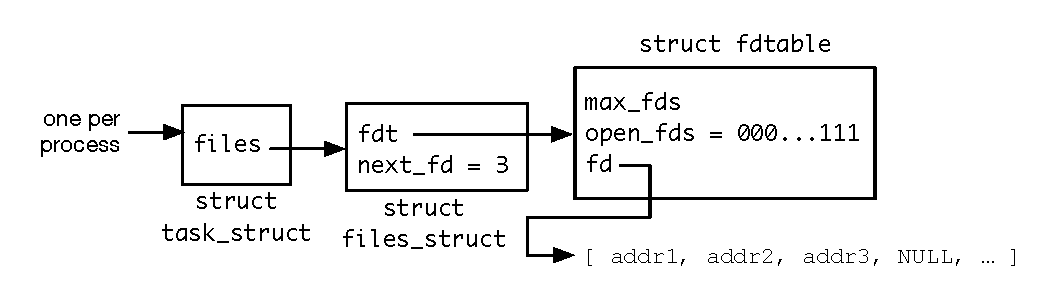
\includegraphics[scale=0.6]{figures/fd_allocation_simple.pdf}
	\centering
	\caption{Simple fd allocation}
	\label{fig:fd_allocation_simple}
\end{figure}

\noindent
Here are the main parts of \cf{alloc\_fd()}:

\begin{lstlisting}
static int 
[*\bfseries alloc\_fd*](unsigned start, unsigned end, unsigned flags)
{
    struct files_struct *files = current->files;
    struct fdtable *fdt;
        
    spin_lock(&files->file_lock);
repeat:
    fdt = [*\bfseries files\_fdtable*](files);
    fd = start;
    if (fd < files->next_fd)
        fd = files->next_fd;
    
    if (fd < fdt->max_fds)
        fd = [*\bfseries find\_next\_fd*](fdt, fd);

    error = -EMFILE;
    if (fd >= end)
        goto out;
    ...
    error = [*\bfseries expand\_files*](files, fd);
    if (error)
        goto repeat;
out:
    spin_unlock(&files->file_lock);
    return error;
}
\end{lstlisting}

\noindent
The function sets \cf{fd} to \cf{start} which is "\cf{0}" (\textbf{dup???}) and sets it to \cf{fd\_next}. The next line looks confusing but I think that's also related to expand\_files() in that we may have set fd to a value beyond what we can actually store so we'll need to expand. Need to confirm.

I always get confused when I see \cf{expand\_files()} and associate it with \cf{file} structures. We are only talking about expansion of the ability to store more file descriptors. 

If we are out of space, the kernel will call \cf{expand\_files()} to add more space. There are two checks at the top of the function. They first is to see if space is actually needed. The second checks against the file descriptor limit.

\begin{lstlisting}
static int 
[*\bfseries expand\_files*](struct files_struct *files, unsigned int nr)
{
    struct fdtable *fdt;

    fdt = [*\bfseries files\_fdtable*](files);

    if (nr < fdt->max_fds) /* Do we need to expand? */
        return expanded;
    
    if (nr >= sysctl_nr_open) /* Can we expand? */
        return -EMFILE;
    
    expanded = [*\bfseries expand\_fdtable*](files, nr);
    return expanded;
}
\end{lstlisting}

\noindent
The allocation of a new file descriptor table occurs in \cf{alloc\_fdtable()}. A call is then made to \cf{copy\_fdtable()} to copy the contents of the old table over to the new.

\begin{lstlisting}
static int 
[*\bfseries expand\_fdtable*](struct files_struct *files, unsigned int nr)
{
    struct fdtable *new_fdt, *cur_fdt;

    new_fdt = [*\bfseries alloc\_fdtable*](nr);
    cur_fdt = [*\bfseries files\_fdtable*](files);
    [*\bfseries copy\_fdtable*](new_fdt, cur_fdt);
}
\end{lstlisting}

\noindent
\textbf{XXX --- should I really go much more into detail here? Feels like I should show how the structures are linked or grown etc but perhaps come back here when I know big this damn thing becomes???}

%---------------------------------------------------------------------------------------------------------------------------------------------------------------------

\subsection{Allocating a \cf{file} Structure}\label{filetable-expand}

After a file descriptor has been allocated and pathname resolution is complete, it's time to allocate a \cf{file} structure. This is done through the following sequence of calls:

\small
\bigskip 
\cf{path\_openat()} $\rightarrow$ \cf{alloc\_empty\_file()} $\rightarrow$ \cf{\_\_alloc\_file()}

\vspace{1pt}
\hspace{1.37in}$\rightarrow$ \cf{kmem\_cache\_zalloc(filp\_cachep, GFP\_KERNEL)}
%\\~\\
    
\bigskip
\normalsize

\noindent
This path is very straightforward. Simply allocate and initialize the structure.

%---------------------------------------------------------------------------------------------------------------------------------------------------------------------

\subsection{KGDB -- Viewing File Descriptor Allocation}

Section \ref{fd-analyze} showed how the kernel structures are linked together after a file had been opened. In this example, we'll walk through the process of opening a file.

First of all we'll set a breakpoint to be hit if the file being opened is "\cf{lorem-ipsum}" as follows:

\begin{lstlisting}
(gdb) [*\bfseries br do\_sys\_openat2 if \$\_streq(filename, "lorem-ipsum")*]
\end{lstlisting}

\noindent
Now that the breakpoint is set, we'll execute our command:

\begin{lstlisting}
(gdb) [*\bfseries cat "lorem-ipsum"*]
\end{lstlisting}

\noindent
and wait for the breakpoint to be hit at which point we'll check the \cf{filename} argument:

\begin{lstlisting}
Thread 2 hit Breakpoint 17, [*\bfseries do\_sys\_openat2*] (dfd=-100, 
    filename=0x7ffc4bd32785 "lorem-ipsum", 
    how=how@entry=0xffffc90000fd7e80) at fs/open.c:1261
1261	{
(gdb) [*\bfseries p filename*]
$104 = 0x7ffc4bd32785 "lorem-ipsum"
\end{lstlisting}

\noindent
At this point, we'll set a breakpoint in \cf{alloc\_fd()} and enter "\cf{c}" to continue execution. You will need to check the stack backtrace when you hit the breakpoint as other processes will likely be opening files at the same time. When we get to the right processes, you can see the \cf{start} and \cf{end} arguments. Since we are simply opening the file, we'll get the lowest possible file descriptor.

\begin{lstlisting}
(gdb) [*\bfseries bt 1*]
#0  [*\bfseries alloc\_fd*] (start=start@entry=0, end=1024, flags=32768) 
    at fs/file.c:501
\end{lstlisting}

\noindent
Steeping through \cf{alloc\_fd()} gets some interesting results. First of all:

\begin{lstlisting}
(gdb) [*\bfseries n*]
501		struct files_struct *files = current->files;
(gdb) [*\bfseries p files*]
$122 = <optimized out>
\end{lstlisting}

\noindent
we can't see the value of \cf{files} since it's optimized out. Why this is the case, I don't know. We can single step

\begin{lstlisting}
508		fdt = files_fdtable(files);
(gdb)[*\bfseries  n*]
510		if (fd < files->next_fd)
(gdb) [*\bfseries p fd*]
$123 = 0
(gdb) [*\bfseries n*]
514			fd = find_next_fd(fdt, fd);
(gdb) [*\bfseries p fd*]
$124 = 3
\end{lstlisting}

\noindent
Note that \cf{fd} is set to the value of \cf{start} (= 0) at the start of the function. We find the lowest available file descriptor value (3 as expected) but then we continue as shown below:

\begin{lstlisting}
(gdb) [*\bfseries n*]
521		if (fd >= end)
(gdb) [*\bfseries n*]
524		error = expand_files(files, fd);
(gdb) [*\bfseries s*]
expand_files (files=files@entry=0xffff888100d26680, 
nr=nr@entry=3) at fs/file.c:217
217	{
(gdb) [*\bfseries n*]
225		if (nr < fdt->max_fds)
(gdb) [*\bfseries n*]
246		return expanded;
\end{lstlisting}

\noindent
It seems unusual that we'll enter \cf{expand\_files()} when we know that we still have space but a check is made at the top of the function so the function returns straightaway. We then set "\cf{files->next\_fd = fd + 1}" and return the file descriptor just allocated (3) to the caller.

%%%%%%%%%%%%%%%%%%%%%%%%%%%%%%%%%%%%%%%%%%%%%%%%%%%%%%%%%%%%%%%

\section{Pathname Resolution}\label{pathname-resolution}

This section describes the implementation of \textit{pathname resolution} which takes a pathname and walks through it one component at a time in order to return an inode for the last component. It's one of the more complex pieces of filesystem code in the kernel as it must handle everything from "." to "..", symbolic links and potentially moving from one filesystem to another across mount points. It can also result in many calls into one or more filesystems often resulting in reads from disk if the dcache and inode caches do not contain requested data. It was also one of the most complex paths to follow in the kernel using breakpoints with \cf{gdb} trying to understand how it all worked. XXX

Many Linux system calls take a a pathname as an argument. This pathname can either a single name representing one of the Linux file types (regular file, directory, symlink etc) or can consist of one or more \textit{components} separated by "/" (or multiple slashes) and perhaps ending with a file type other than a directory depending on the system call being invoked.

Each process has the notion of a \textit{current working directory} that is assigned when the process is created or inherited from its parent process. When logging into Linux, your current working directory is set to your home directory as specified in \cf{/etc/passwd}. An absolute pathname starts with "/" (the \textit{root directory}) whereas a relative pathname starts with a file or directory that is in the \textit{current working directory}. Pathname resolution starts with an absolute or relative pathname unless one of the \cf{*at} system calls is invoked such as \cf{openat(2)}.

The last chapter covered different kernel structures and caches for file names (dcache) and files (inodes). The hope is that during pathname resolution, many of the components within the path will already be in one of these caches to avoid the filesystem having to read what could potentially be many different structures from disk.

A large part of opening a file involves resolving the pathname to get to the base filename. Where to start the search depends on how the pathname is formed (relative or absolute as described above). The following information may influence both:

\begin{enumerate}
	\item A process inherits its root directory from its parent and usually, it will be the root directory of the Linux file hierarchy.
	\item A process may get a different root directory through use of the \cf{chroot(2)} system call, or may temporarily use a 
	different  root  directory by using the \cf{openat2(2)} system call with the \cf{RESOLVE\_IN\_ROOT} flag set.
	\item A process may get an entirely private mount namespace if it, or one of  its  ancestors, was  started 
	by an invocation  of  the pathname.\textbf{XXX -- what does this mean?}
	\item The current working directory is also inherited from the parent process but this can be changed by using the \cf{chdir(2)} 
	system call.
\end{enumerate}

\noindent
The \cf{path\_resolution(7)} manpage describes the general process of resolving a pathname down to a file. I recommend that you start with this manpage to understand the general process that the kernel will follow before the chapter describes the kernel functions and structures that provide pathname resolution. For now, \cf{path\_resolution(7)} describes the process as three steps which are rephrased here:

\vspace{0.25cm}
\noindent
\textbf{Step 1 -- Start of the resolution process}

\vspace{0.25cm}
\noindent
The first steps is to identify where the search starts from. If the pathname starts with a "/" it's an absolute pathname and resolution will start from the root directory of the process unless one of the \cf{*at} system calls is used in which case a new root directory is chosen. If the pathname doesn't start with "/", it's a relative pathname and starts at the current working directory. The \textit{current lookup directory} is set to one of these two directories.

\vspace{0.25cm}
\noindent
\textbf{Step 2 --  Walking along the path}

\vspace{0.25cm}
\noindent
For each component of the pathname, where a component is a substring delimited by one or more '/' characters, the component is \textit{looked up} in the current lookup directory. If the component is delimited by '/' characters it cannot be the final component.

\vspace{0.25cm}
\noindent
\textbf{Step 3 -- Finding the final entry}

\vspace{0.25cm}
\noindent
The lookup of the final component of the pathname is no different than all other components, as described in the previous step, other than it has no terminating "/" character. Whether this component is a directory or other file type is not relevant as far as pathname resolution is concerned. Whether it is the correct type of file will be determined by the type of system call and therefore the caller of pathname resolution.

\vspace{0.25cm}
We covered how the initial file descriptor array is stored and referenced from the \cf{task\_struct} in section XXX. This is structured in a way that it's quick and easy to get the next file descriptor unless another file table needs to be allocated in which case a call to \cf{expand\_files()} is made. Section \ref{fd-analyze} also showed how to find file descriptor entries using \cf{gdb} using the first file descriptor table.

%------------------------------------------------------------------------------------------------------------------------------------------------------------------------

\subsection{Setting the Stage for Pathname Resolution}\label{pathname-set}

The current status of pathname resolution is stored in the allocated \cf{nameidata} structure. A function called \cf{namei()} (convert a a name to an inode) was originally the name for pathname resolution in UNIX. In fact you can view the source to \cf{namei()} in 6th Edition UNIX in the file \cf{sys/ken/nami.c}. Yes, that's Ken as in Ken Thompson, one of the founders of UNIX and now one of the creators of the language Golang. 

\begin{table}[h]
\begin{tabular}{ll}
\parbox[l]{0.6in}{
\includegraphics[scale=0.8]{figures/src-xref.pdf}} & \parbox[l]{4in}{\small{\cf{nameidata} is defined in \cf{include/linux/nameidata.h} and \cf{path} is defined in \cf{include/linux/path.h}. Most of the functions described in this section are in \cf{fs/namei.c}.}}
\end{tabular}
\end{table}

\noindent
Here is part of the \cf{nameidata} structure. It has a lot of elements so only the most important fields in the structure will be described:

\begin{lstlisting}
struct [*\bfseries nameidata*] {
    struct path             path;
    struct qstr             last;
    struct path             root;
    struct inode            *inode;
    unsigned int            flags, state;
    unsigned                seq, m_seq, r_seq;
    int                     last_type;
    unsigned                depth;
    int                     total_link_count;
    struct saved {
        struct path         link;
        struct delayed_call done;
        const char          *name;
        unsigned            seq;
    } *stack, internal[EMBEDDED_LEVELS];
    struct filename         *name;
    struct nameidata        *saved;
    unsigned                root_seq;
    int                     dfd;
    kuid_t                  dir_uid;
    umode_t                 dir_mode;
} 
\end{lstlisting}

\noindent
Here are the most important fields:

\begin{itemize}
	\item \cf{path} -- this is a \cf{path} structure contains a \cf{vfsmount} and a \cf{dentry} structure. Together, they record the 
		current status of pathname resolution. Initially the \cf{dentry} field is the starting point of the path walk 
		such as the root directory the or the current working directory. The \cf{mnt} field references the filesystem which
		is currently being traversed. This structure is updated on each step through pathname resolution and potentially cross
		mount points. For example, if we cross a mount point, \cf{mnt} will be updated to reference the \textit{mounted on}
		filesystem.
	\item \cf{last} -- this is the next component to search for. Strictly speaking, it's actually the remaining part of the
		pathname to search for and the hash len field is the number of characters in the component that will be searched 
		for. Each time we return from \cf{walk\_component()} it gets reduced by one directory component (ignoring 
		symlinks for now). On return from \cf{link\_path\_walk} it will contain the last component in the path.
	\item \cf{root} -- a reference to the root of the calling process's tree. This is only set for absolute pathnames since it
		is assumed that most callers of this function will pass relative pathnames. \textbf{Why bother?}
	\item \cf{inode} -- the current directory where we are currently looking. The \cf{step\_into()} function will result in this 
		field being updated as pathname resolution moves from one directory to another. \textbf{why bother? it's in path->dentry}
	\item \cf{state} -- 
	\item \cf{saved} -- used for symlink / recursion - explain later.
	\item \cf{last\_type} -- \cf{LAST\_NORM}, \cf{LAST\_ROOT}, \cf{LAST\_DOT} or \cf{LAST\_DOTDOT}. This field is
		set to \cf{LAST\_ROOT} at the start of pathname resolution.  XXX it's not set in many places. go look.
\end{itemize}

\noindent
The second structure that is used during pathname resolution is the \cf{path} structure:

\begin{lstlisting}
struct path {
    struct vfsmount *mnt;
    struct dentry   *dentry;
}
\end{lstlisting}

\noindent
This structure refers to a component in the path being resolved and records where the kernel is during that process. \textbf{I suspect it's the same for mount since a mount path is passed. It's allocated on the stack inside \cf{do\_mount}}

%---------------------------------------------------------------------------------------------------------------------------------------------------------------------

\subsection{Initialization Structures And Starting The Process}

When entering \cf{do\_filp\_open()}, a call is made to \cf{set\_nameidata()} to initialize the \cf{nameidata} structure. Most fields are just initialized to NULL/0 values. There is no attempt at this point to set the starting inode as root (absolute search) or the current working directory (relative search).

Figure \ref{fig:cwd-and-root-directory} is a modified version of figure \ref{fig:open-fd-alloc} and shows how pathname handling code gets access to the root directory for absolute pathnames and the current working directly for relative pathnames. The \cf{fs} field in the \cf{task\_struct} references a \cf{fs\_struct} structure in which the kernel can easily get access to one or the other through directories. 

\begin{figure}[h]
	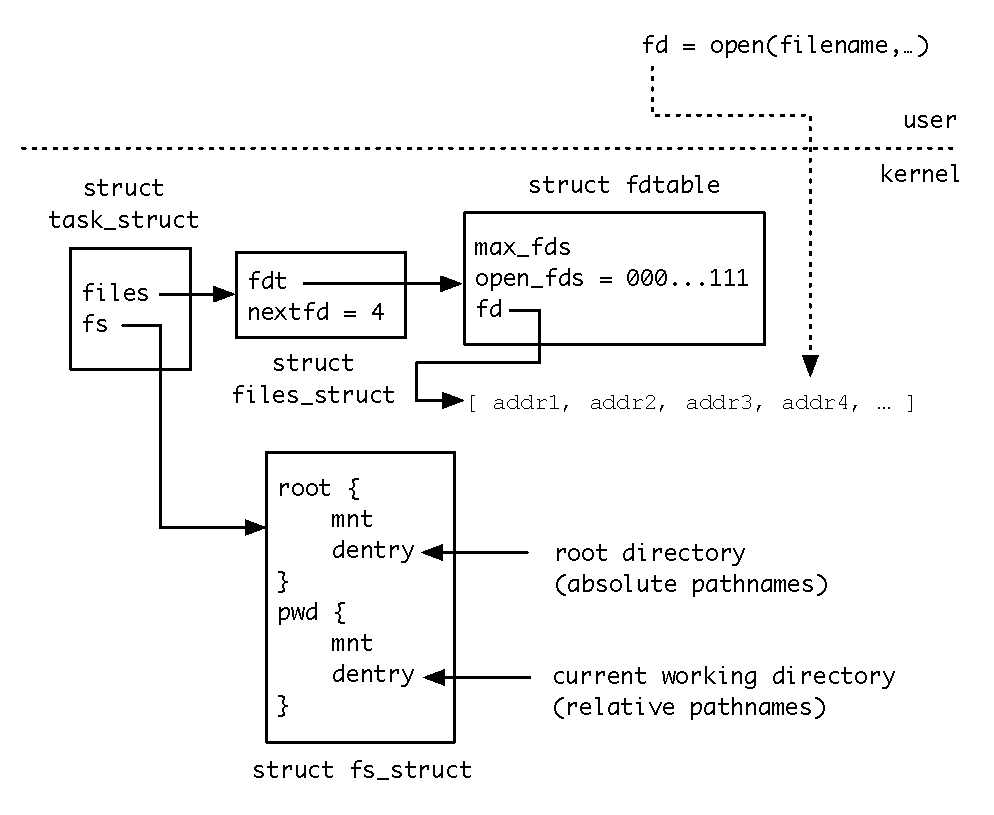
\includegraphics[scale=0.6]{figures/cwd-and-root-directory.pdf}
	\centering
	\caption{TBD}
	\label{fig:cwd-and-root-directory}
\end{figure}

\begin{lstlisting}
struct fs_struct *fs = current->fs;

nd->root = fs->root;                    /* to get the root */

nd->path = fs->pwd;                     /* to get the CWD */
nd->inode = nd->path.dentry->d_inode;
\end{lstlisting}

\noindent
Note that both contain the same fields as the \cf{path} field of the \cf{nameidata} structure.

After initializing the \cf{nameidata} structure, \cf{filp\_open()} calls \cf{path\_openat()} which performs additional initialization before calling the main pathname walking function \cf{link\_path\_walk()}. Here is a fragment of the code:
 
\begin{lstlisting}
static struct file *
[*\bfseries path\_openat*](struct nameidata *nd,
            const struct open_flags *op, unsigned flags)
{   
    struct file *file;
    int error;
        
    file = [*\bfseries alloc\_empty\_file*](op->open_flag, current_cred());
    ...
    } else {
        const char *s = [*\bfseries path\_init*](nd, flags);
        while (!(error = [*\bfseries link\_path\_walk*](s, nd)) &&
               (s = [*\bfseries open\_last\_lookups*](nd, file, op)) != NULL)
            ;
        if (!error)
            error = [*\bfseries do\_open*](nd, file, op);
        terminate_walk(nd);
    }
\end{lstlisting}

\noindent
The first step is to call \cf{alloc\_empty\_file()} to allocate a new \cf{file} structure. This will result in a call to \cf{kmem\_cache\_zalloc()} to allocated the structure and then the fields are initialized. 

The final initialization function to call is \cf{path\_init()}. Among other things (XXX) this function will locate the root directory or current working directory and set the appropriate fields in the \cf{nameidata} structure. \textbf{XXX - it does a lot of other stuff too}.

Once pathname resolution is complete, a call is made to \cf{restore\_nameidata()} which restores the old \cf{nameidata} structure that was saved during \cf{set\_nameidata()}. \textbf{XXX - need to understand why this is being done}

Need to figure out what \cf{current->nameidata} - looks like the current one is saved? help continue from where we are?

% https://patchwork.kernel.org/project/linux-fsdevel/patch/1429553588-24764-2-git-send-email-viro@ZenIV.linux.org.uk/

%------------------------------------------------------------------------------------------------------------------------------------------------------------------------

\subsection{The Nitty Gritty of Pathname Resolution}

Pathnames can contain a mix of directories and end with either a directory or a regular file depending on which system call is being invoked (and assuming a valid pathname of course). They can also contain the directories "." and ".." referring to the current directory and the directory above where "we are now"

Once everything is initialized, \cf{path\_openat()} will call \cf{link\_path\_walk()} which is the function that iterates through each component of the pathname as shown in figure \ref{fig:link-path-walk}. You can see that the \cf{name} argument contains the pathname that is being passed to \cf{ls(2)}.

\begin{figure}[h]
	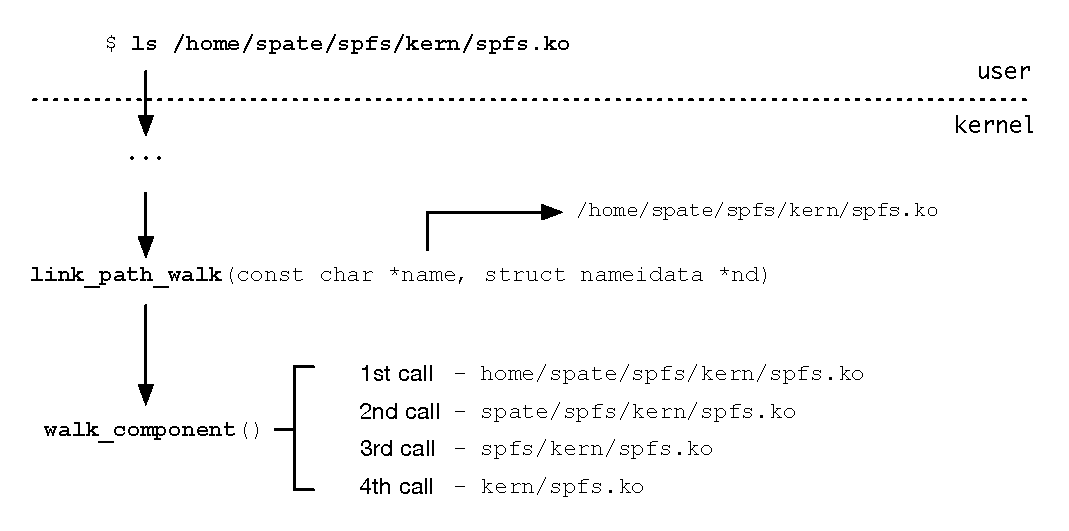
\includegraphics[scale=0.6]{figures/link-path-walk.pdf}
	\centering
	\caption{Repeated calls to \cf{walk\_component()}}
	\label{fig:link-path-walk}
\end{figure}

Inside \cf{link\_path\_walk()} there are several things to do. First is to remove any "/" characters from the front of the remaining path. Next is to check that the directory has execute permission (\cf{may\_lookup()}. Then the function loops through the pathname one component at a time until it reaches the last component.

\begin{lstlisting}
static int 
[*\bfseries link\_path\_walk*](const char *name, struct nameidata *nd)
{
    while (*name=='/')
        name++;

    for(;;) { /* loop for ecah component */
        mnt_userns = [*\bfseries mnt\_user\_ns*](nd->path.mnt);
        err = [*\bfseries may\_lookup*](mnt_userns, nd);

        hash_len = [*\bfseries hash\_name*](nd->path.dentry, name);
        ...
        handle all hash stuff!
        ...

        if (unlikely(!*name)) {
            /* handle symlinks */
            link = [*\bfseries walk\_component*](nd, 0);
        } else {
            /* not the last component */
            link = [*\bfseries walk\_component*](nd, WALK_MORE);
        }
}
\end{lstlisting}

\noindent
For the last component, \cf{nd->last} and \cf{nd->last\_type} are set but no call is made to \cf{walk\_component()}. Handling the last component will be done by the caller of \cf{link\_path\_walk()}.

\textbf{Really need to figure out all the hashing stuff as it penetrates everything.} A call is made to \cf{walk\_component()} for each component in the path apart from the last one (XXX) as this may be a file that doesn't exist and we may be creating it or just stat. Need to find out more here.

Here are the steps performed by \cf{walk\_component()}:

\begin{lstlisting}
static const char *
[*\bfseries walk\_component*](struct nameidata *nd, int flags)
{       
    struct dentry *dentry;
    struct inode *inode;
    unsigned seq;

    if (unlikely(nd->last_type != LAST_NORM)) {
        if (!(flags & WALK_MORE) && nd->depth)
            put_link(nd);
        return [*\bfseries handle\_dots*](nd, nd->last_type);
    }       
    dentry = [*\bfseries lookup\_fast*](nd, &inode, &seq);
    if (unlikely(!dentry)) {
        dentry = [*\bfseries lookup\_slow*](&nd->last, nd->path.dentry, 
                     nd->flags);
    }
    if (!(flags & WALK_MORE) && nd->depth)
        [*\bfseries put\_link*](nd);
    return [*\bfseries step\_into*](nd, flags, dentry, inode, seq);
}
\end{lstlisting}

\noindent
The \cf{flags} argument can be one of:

\begin{itemize}
	\item \cf{WALK\_TRAILING} -- this indicates that we are on the final component of the lookup. A check is made on the
		user-space flag \cf{LOOKUP\_FOLLOW} to determine whether follow it when the last component is a symlink If
		this is the case, a call is made to \cf{may\_follow\_link()} to check if we have privilege to follow the link.
	\item \cf{WALK\_MORE} --  this flag indicates that it is yet too early to release the current symlink. This will
		further described in section \ref{pathname-symlinks}.
	\item \cf{WALK\_NOFOLLOW} -- this flag specifies that if a symlink is found it should not be followed.
\end{itemize}

\noindent
The dentry for the component being looked up will either already be in the dcache or a call will need to be made into the filesystem. To check if it's in the cache, \cf{walk\_component()} calls \cf{lookup\_fast()} and if that fails to find it in the cache it then calls \cf{lookup\_slow()}. \textbf{XXX - it says "unlikely" before calling slow implying ... well ..??} Really looks like a locking issue too. fast takes less locks. slow takes more. just google search.

To see if the dentry is already in the dcache, a call is made to \cf{lookup\_fast()} which in turn calls \cf{\_\_d\_lookup\_rcu()}. Inside this function, the right dcache hash bucket is located and scanned to see if there is a matching dentry:

\begin{lstlisting}
struct dentry *
[*\bfseries \_\_d\_lookup\_rcu*](const struct dentry *parent,
               const struct qstr *name, unsigned *seqp)
{
    u64 hashlen = name->hash_len;
    const unsigned char *str = name->name;
    struct hlist_bl_head *b = [*\bfseries d\_hash*](hashlen_hash(hashlen));
    struct hlist_bl_node *node;
    ...
    [*\bfseries hlist\_bl\_for\_each\_entry\_rcu*](dentry, node, b, d_hash) {
        ...
            if ([*\bfseries dentry\_cmp*](dentry, str, 
                           [*\bfseries hashlen\_len*](hashlen)) != 0)
                continue;
        }
        *seqp = seq;
        return dentry; 
}
\end{lstlisting}

\noindent
The \cf{str} argument passed to \cf{dentry\_cmp()} is the remaining path in our search but we only compare against the correct number of characters for the current component. For example, \cf{str} could be "\cf{spfs/kern/spfs.ko}" but \cf{hashlen\_len(hashlen)} will return "4" which is the length of "\cf{spfs}".

As a reminder, we have traversed through the following path trying to find the current component in the dcache:

\small
\bigskip 
\cf{link\_path\_walk()} $\rightarrow$ \cf{walk\_component()}  $\rightarrow$ \cf{lookup\_fast()} 

\vspace{1pt}
\hspace{1.37in}$\rightarrow$ \cf{\_\_d\_lookup\_rcu()} 
%\\~\\
    
\bigskip
\normalsize
\noindent
Single stepping through \cf{\_\_d\_lookup\_rcu()} , we hit the line where we're comparing the string we're looking for against dentries in the hash bucket where it will be found (if present):

\begin{lstlisting}
(gdb) [*\bfseries n*]
2369     if (dentry_cmp(dentry, str, hashlen_len(hashlen)) != 0)
\end{lstlisting}

\noindent
Here is the string being passed:

\begin{lstlisting}
(gdb) [*\bfseries p str*]
$3 = (const unsigned char *) 0xffff888100f90021 
                                 "home/spate/spfs/kern/spfs.ko"
\end{lstlisting}

\noindent
But we only want to compare each dentry found against the string "\cf{home}". As mentioned above, \cf{hashlen\_len(hashlen)} will return "4" allowing us to compare only what we need and not the rest of the string.

Assuming the dentry is found (fast or slow path), \cf{walk\_component()} makes a call is made to \cf{step\_into()} which calls \cf{handle\_mounts()} to see if a mount point is being crossed. In this case, a new \cf{path} structure is created which references to dentry for the root of the mounted-on filesystem and a reference to the new \cf{vfsmount}. 

It also handles the case of the current component being a symbolic link in which a call is made to \cf{pick\_link()} to handle it. If neither of these cases exits, \cf{nd->path} is updated and return is made to \cf{walk\_component()}. Oddly enough, if we are not crossed a mount point, it is still \cf{handle\_mounts()} that updates \cf{path->dentry} to the new directory from where to continue searching.

%------------------------------------------------------------------------------------------------------------------------------------------------------------------------

\subsection{Callers of \cf{link\_path\_walk()}}

There are only three callers of \cf{link\_path\_walk()} but these three functions are in turn used by many paths throughout the kernel as shown in figure \ref{fig:link-path-walk-callers}.

\begin{figure}[h]
	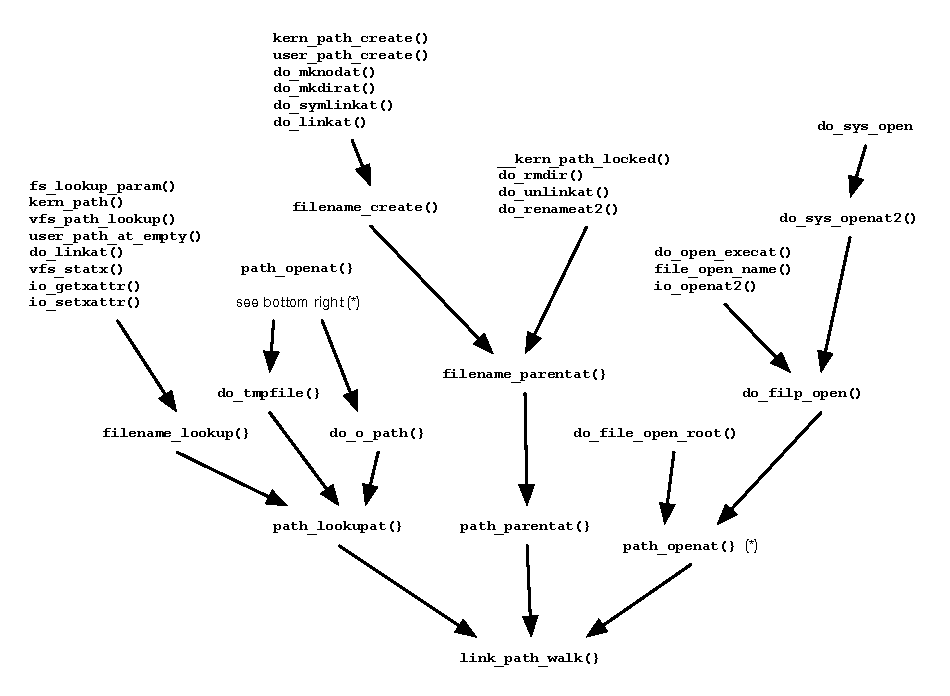
\includegraphics[scale=0.8]{figures/link-path-walk-callers.pdf}
	\centering
	\caption{Callers of \cf{link\_path\_walk()}}
	\label{fig:link-path-walk-callers}
\end{figure}

\noindent
This figure will come in helpful when following several system call paths. For example, callers of \cf{filename\_create()} are typically system calls that involve creating a file such as a directory, symbolic link or hard link. For \cf{open(2)}, \cf{creat(2)} and similar system calls, see the right hand side of the figure.

%------------------------------------------------------------------------------------------------------------------------------------------------------------------------

\subsection{More on Hashing}\label{dcache-hash} 

\textbf{Described the algorithms in more detail}

%------------------------------------------------------------------------------------------------------------------------------------------------------------------------

\subsection{Handling a dcache Miss}

If \cf{\_\_d\_lookup\_rcu()} fails to find the name in the dcache, \cf{\_\_lookup\_slow()}, a call will likely be made into the filesystem to read the component from disk. It is "likely" because a check is made again to see if the name is in the dcache before a \cf{lookup()} filesystem call is made. The extra dcache check is made because the first scan takes place without locks and the file could have been added in the meantime. This time however, a shared lock (\cf{i\_rwsem}) is taken on the directory inode. Entries are added to the dcache by taking an exclusive lock on \cf{i\_rwsem}.

\begin{lstlisting}
static struct dentry *
[*\bfseries \_\_lookup\_slow*](const struct qstr *name,
                    struct dentry *dir,
                    unsigned int flags)
{
    struct dentry *dentry, *old;
    struct inode *inode = dir->d_inode;

    dentry = [*\bfseries d\_alloc\_parallel*](dir, name, &wq);
    if (unlikely(![*\bfseries d\_in\_lookup*](dentry))) {
        int error = [*\bfseries d\_revalidate*](dentry, flags);
        ...
            } else {
        old = inode->i_op->[*\bfseries lookup*](inode, dentry, flags);
        d_lookup_done(dentry);
        if (unlikely(old)) {
            dput(dentry);
            dentry = old;
        }
    }
    return dentry;
}
\end{lstlisting}

\noindent

\textbf{XXX -- need to flush out this stuff}

% call to __lookup_slow
% why we check the dcache again
% alloc dentry
% inode->i_op->lookup

%------------------------------------------------------------------------------------------------------------------------------------------------------------------------

\subsection{Crossing mount points}

Before digging back into the source code, consider the file hierarchy in figure \ref{fig:pathname-tree}:

\begin{figure}[h]
	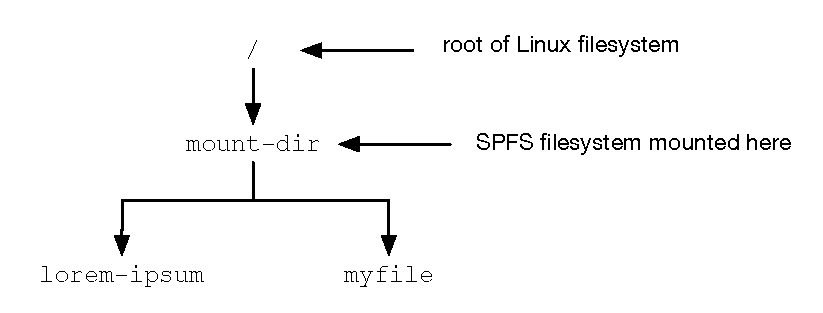
\includegraphics[scale=0.6]{figures/pathname-tree.pdf}
	\centering
	\caption{Simple file hierarchy with a mounted filesystem}
	\label{fig:pathname-tree}
\end{figure}

\noindent
The root filesystem has a directory called "\cf{mount-dir}" on to which a filesystem is mounted. Inside this mounted filesystem there are two files. Figure \ref{fig:pathname-dentries} shows the dentries for the five files shown here. The \cf{d\_flags} field is set to \cf{DCACHE\_MOUNTED} indicating that a filesystem is mounted on top of it. Strictly speaking, this is a hint and is not always set but we will cover that later.

\begin{figure}[h]
	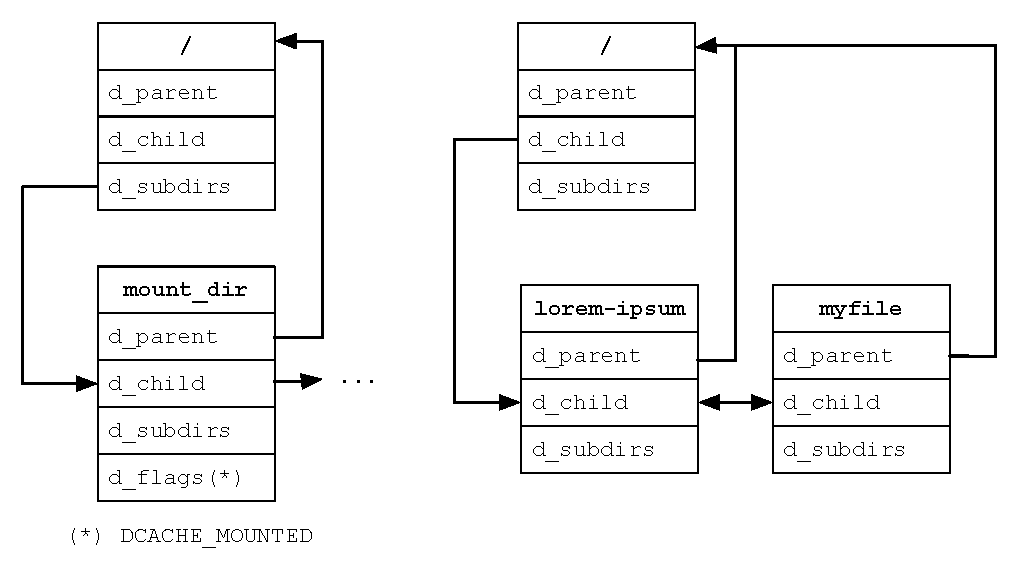
\includegraphics[scale=0.6]{figures/pathname-dentries.pdf}
	\centering
	\caption{dentries for the simple file hierarchy}
	\label{fig:pathname-dentries}
\end{figure}

\noindent
All dentries representing directories maintain a doubly linked list headed by the d\_subdirs field that runs through the child dentries' \cf{d\_child} fields. Each child's \cf{d\_parent} pointer points to its parent unless it's the root dentry in which case it points to itself (see the \cf{IS\_ROOT()} macro in \cf{include/linux/dcache.h}. Note that there is no direct pointer from the \cf{mount-dir} dentry to the root of the SPFS filesystem. That is done through \cf{mount\_hashtable} and will be covered below when we look further into the code.

As we scan through the pathname one component at a time, we lookup its dentry. If this is a directory and a filesystem is mounted on top of it, it's easy to determine by checking the dentry flags field. There can be one of the following flags that relate to mounted filesystems:

\begin{itemize}
	\item \cf{DCACHE\_MOUNTED} -- this flag indicates that there is a filesystem mounted on top of this directory. 
	\item \cf{DCACHE\_NEED\_AUTOMOUNT} -- if this flag is set we need to automount a filesystem on this directory 
		before we can traverse into it. 
\end{itemize}

\noindent
There is no direct link from the dentry for \cf{mount-dir} to the root of the mounted filesystem. So even though the dentry for \cf{mount-dir} has the \cf{DCACHE\_MOUNTED} flag set, XXX

SVR4-based UNIX systems encoded which filesystems were mounted where through the use of fields in the \cf{vnode} structure (equivalent of the Linux \cf{inode} structure. Linux is different in that this information is recorded in the dcache with the \cf{dentry} structure.

NOTE --- XXX

This is used to get to a root dentry from a mounted on dentry (DCACHE\_MOUNTED) need to confirm this

\noindent
Here is the path followed from \cf{walk\_component()}:

\small
\bigskip 
\cf{walk\_component()} $\rightarrow$ \cf{step\_into()} $\rightarrow$  \cf{handle\_mounts()} 

\vspace{1pt}
\hspace{1.53in}
$\rightarrow$  \cf{traverse\_mounts()} $\rightarrow$ \cf{\_\_traverse\_mounts()}
\bigskip 
\normalsize

\noindent
\cf{pick\_link()} handles symlinks.

The \cf{path} structure is defined in \cf{include/linux/path.h} and contains two members:

\begin{lstlisting}
struct path {
    struct vfsmount *mnt;    - which FS tree we are in now
    struct dentry *dentry;   - root node or is it the CWD?
}
\end{lstlisting}

\noindent
where the \cf{dentry} references the root of the filesystem.

Here is the source code in \cf{\_\_traverse\_mounts()} that covers a filesystem mounted on this directory. If we get a vfsmoutn back from \cf{lookup\_mnt()}, we release the current dentry where we're searching (\cf{dput(path->dentry)} and set it to the the dentry for the root of the filesystem that's mounted on top of this directory (\cf{mounted->mnt\_root}).

\begin{lstlisting}
if (flags & DCACHE_MOUNTED) {   // something's mounted on it..
    struct vfsmount *mounted = [*\bfseries lookup\_mnt*](path);
    if (mounted) {      // ... in our namespace
        [*\bfseries dput*](path->dentry);
        if (need_mntput)
            [*\bfseries mntput*](path->mnt);
        path->mnt = mounted;
        path->dentry = [*\bfseries dget*](mounted->mnt_root);
        flags = path->dentry->d_flags;
        need_mntput = true;
    }   
}  
\end{lstlisting}

\noindent
The \cf{lookup\_mnt()} function in turn calls \cf{\_\_lookup\_mnt()} which walks the mount hash table to locate the root dentry for the mounted filesystem:

\begin{lstlisting}
struct mount *
[*\bfseries \_\_lookup\_mnt*](struct vfsmount *mnt, struct dentry *dentry)
{
    struct hlist_head *head = [*\bfseries m\_hash*](mnt, dentry);
    struct mount *p;

    [*\bfseries hlist\_for\_each\_entry\_rcu*](p, head, mnt_hash)
        if (&p->mnt_parent->mnt == mnt && 
                                   p->mnt_mountpoint == dentry)
            return p;
    return NULL;
}
\end{lstlisting}

\noindent
The goal of \cf{m\_hash()} is to return the correct hash bucket to search for the mount XXX we need.  \cf{mount\_hashtable} is defined in \cf{namespace.c} and described in section \textbf{dcache-links}. 

\noindent
Here are the first few fields of the mount structure:

\begin{lstlisting}
struct mount {
    struct hlist_node [*\bfseries mnt\_hash*];
    struct mount *mnt_parent;
    struct dentry *mnt_mountpoint;
    struct vfsmount mnt;
    ...
\end{lstlisting}

\noindent
so the \cf{mount} structures are held in a list accessed through the first field \cf{mnt\_hash}.

Back in  \cf{\_\_traverse\_mounts()}, once the new mount is found, the \cf{path} structure is updated to reference the new filesystem that we are entering into as well as the dentry for the root of this tree.

%------------------------------------------------------------------------------------------------------------------------------------------------------------------------

\subsection{Handling Symlinks}\label{pathname-symlinks}

xxx

%------------------------------------------------------------------------------------------------------------------------------------------------------------------------

\subsection{Returning From \cf{link\_path\_walk()}}

Before each call to \cf{walk\_component()}, table \ref{table:path-walk} shows the contents of \cf{nd->last} and the local variable "\cf{name}".

\begin{table}[h]
\begin{center}
\begin{tabular}{|m{0.065\textwidth}|m{0.45\textwidth}|m{0.4\textwidth}|}
\hline
\rowcolor[gray]{.93}\bf{Call}&\bf{\cf{nd->last.name}}&\bf{\cf{name}}\\
\hline
1&\cf{home/spate/spfs/kern/spfs.ko}&\cf{spate/spfs/kern/spfs.ko}\\
\hline
2&\cf{spate/spfs/kern/spfs.ko}&\cf{spfs/kern/spfs.ko}\\
\hline
3&\cf{spfs/kern/spfs.ko}&\cf{kern/spfs.ko}\\
\hline
4&\cf{kern/spfs.ko}&\cf{spfs.ko}\\
\hline
\end{tabular}
\caption{\small Standard File Descriptors}
\label{table:path-walk}
\end{center}
\end{table}

\noindent
Before returning from \cf{link\_path\_walk()} the \cf{last.name} field of \cf{nd} will be set to \cf{name} and \cf{last.hash\_len} set to the length of the string. This allows the caller to deal with the last component.

There are three callers of \cf{link\_path\_walk()} namely:

\begin{itemize}
	\item \cf{path\_openat()} --  this is used for the \cf{open(2)} system call and is more complex. It will be covered XXX.
	\item \cf{path\_parentat()} -- this function returns the parent directory and the final component to its caller which will 
		typically be creating, removing or renaming a file.
	\item \cf{path\_lookupat()} -- operations such as \cf{stat(2)} come in through this function. It will call \cf{lookup\_last()}
		which in turn calls \cf{walk\_component} for the last component passing \cf{WALK\_TRAILING} as the second argument.
\end{itemize}

\noindent
The  \cf{path\_parentat()} and \cf{path\_lookupat()} functions are described in section XXX. Since this chapter started with opening a file, let's look at what \cf{path\_openat()} does on return from \cf{link\_path\_walk()}. Here is the code surrounding the call to \cf{link\_path\_walk()}:

\begin{lstlisting}
while (!(error = [*\bfseries link\_path\_walk*](s, nd)) &&
       (s = [*\bfseries open\_last\_lookups*](nd, file, op)) != NULL)
    ;
    if (!error)
        error = [*\bfseries do\_open*](nd, file, op);
terminate_walk(nd);
\end{lstlisting}

\noindent
The function loops around the calls to \cf{link\_path\_walk()} and \cf{open\_last\_lookups()} since the last component could be a symlink in which case another call will be made to \cf{link\_path\_walk()}. For the non symlink case, \cf{open\_last\_lookups()} calls \cf{lookup\_fast()} to see if the last component is in the dcache. If not a call is made to \cf{lookup\_open()} to open the file. \textbf{XXX --- need to come back here once I understand where file creation doc will go. there is another section}

%------------------------------------------------------------------------------------------------------------------------------------------------------------------------

\subsection{RCU-walk vs REF-walk}

It was mentioned at the start of the section that pathname resolution was one of the more complex pieces of code in the Linux kernel and despite describing the process at depth, a lot of detail has still been left out. There are a lot of locks to be taken along the way and if components aren't in the dcache, that could mean a lot of calls into the filesystem and typically to disk.

There are actually two modes of pathname resolution, one that attempts to speed things up and a fallback when the fast path isn't available. These modes are:

\begin{itemize}
	\item RCU-walk -- introduced in 2.6.38, RCU allows for a large part of pathname resolution to be performed without
		taking locks. As on-line documenation states, it allows "\textit{a significant part of the entire path walk (including 
		dcache look-up) completely “store-free” (so, no locks, atomics, or even stores into cachelines of common dentries)}.
	\item RCU-walk -- when the kernel can't continue in RCU  mode, it drops into REF-walk which is the older method
		of pathname resolution whereby locks are taken as needed. This results in poor performance on multi-processor
		architectures where multiple threads can be competing for locks at the same time.
\end{itemize}

\noindent
XXX

It's all to do with the \textit{sequence count}. You will see references to a sequence count inside \cf{lookup\_fast()} when called by \cf{walk\_component()} as follows:

\begin{lstlisting}
    dentry = lookup_fast(nd, &inode, &seq);
\end{lstlisting}

\noindent
\textbf{XXX - there are comments in lookup\_fast() indicating that this is really to do with things "changing" underneath us which makes sense if few locks are taken}

There are some stats in the following page - see how to get them

% https://www.infradead.org/~mchehab/kernel_docs/filesystems/path-walking.html - great doc. Explains hash buckets
% https://www.linuxjournal.com/article/7124 - scaling dcache with RCU (reference from above - link broken)

\textbf{one of the docs talks about the callers of path\_link\_walk and talks about what each does with the last component. take a look at that and write about it.}

 %------------------------------------------------------------------------------------------------------------------------------------------------------------------------

\subsection{KGDB -- Setting The Stage For Pathname Resolution}

This example will show how the kernel is entered, everything is set up and the pathname resolution code is entered through a call to \cf{link\_path\_walk()}. There are only three callers of \cf{link\_path\_walk()} but multiple callers of these three functions.

We'll be starting with \cf{filp\_open()} as shown in figure \ref{fig:kgdb-path}.

\begin{figure}[h]
	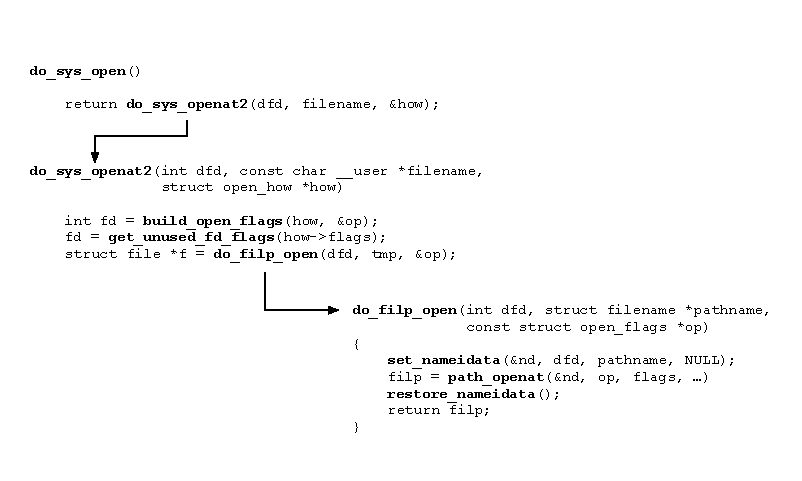
\includegraphics[scale=0.95]{figures/kgdb-path.pdf}
	\centering
	\caption{System call handling for opening a file}
	\label{fig:kgdb-path}
\end{figure}

Linux processes are invoking system calls all of the time therefore setting a breakpoint in \cf{gdb} for one of the more popular system calls (file access for example) will likely be hit by several processes in addition to the one you're tracking. And this is especially true of pathname resolution which is used by multiple different system calls.

Therefore to set a breakpoint you will want to set a \textit{conditional breakpoint}. You can set a breakpoint anywhere but we'll set one in \cf{do\_filp\_open()} after a file descriptor has been allocated:

\begin{lstlisting}
struct file *[*\bfseries do\_filp\_open*](int dfd, struct filename *pathname,
                          const struct open_flags *op)
\end{lstlisting}

\noindent
The \cf{filename} structure has a field called \cf{name} which points to the pathname being looked up. To make sure a breakpoint can be easily set, the following program will be run:

\begin{lstlisting}
$ [*\bfseries cat lorem-ipsum*]
\end{lstlisting}

\noindent
and prior to running the program, a conditional breakpoint can be set as follows ensuring that the breakpoint will only by triggered if a process is accessing the file \cf{lorem-ipsum}. Here is how the breakpoint is set:

\begin{lstlisting}
(gdb) [*\bfseries br do\_filp\_open if \$\_streq(pathname->name, "lorem-ipsum")*]
\end{lstlisting}

\noindent
When the program runs and the breakpoint is triggered, you will see the following in \cf{gdb}:

\begin{lstlisting}
Thread 3 hit Breakpoint 4, do_filp_open (dfd=dfd@entry=-100, 
pathname=pathname@entry=0xffff88810263b000, 
op=op@entry=0xffffc90000fc3dd4) at fs/namei.c:3678
3678	{
(gdb) 
\end{lstlisting}

\noindent
Before going further, we can look at the \cf{task\_struct} for this process to see the root directory and current working directory as follows. One or the other will be used for pathname resolution depending on whether it's an absolute or relative pathname.

\begin{lstlisting}
(gdb) [*\bfseries p \$lx\_current()->fs->root.dentry->d\_name.name*]
$40 = (const unsigned char *) 0xffff88812f9ad578 "/"
(gdb) [*\bfseries p \$lx\_current()->fs->pwd.dentry->d\_name.name*]
$39 = (const unsigned char *) 0xffff88811f163878 "spate"
\end{lstlisting}

\noindent
The stack backtrace is shown below which will correspond to the calls shown in figure \ref{fig:kgdb-path}. All functions are shown in bold. You can see the low-level functions called as part of system call handling and resulting in a call to \cf{do\_sys\_open()}.

\begin{lstlisting}
(gdb) [*\bfseries bt 3*]
#0  [*\bfseries do\_filp\_open*] (dfd=dfd@entry=-100, 
    pathname=pathname@entry=0xffff888100870000, 
    op=op@entry=0xffffc90000d57e04) at fs/namei.c:3678
#1  [*\bfseries do\_sys\_openat2*] (dfd=-100, filename=<optimized out>, 
    how=how@entry=0xffffc90000d57e48) at fs/open.c:1275
#2  [*\bfseries do\_sys\_open*] (mode=<optimized out>, 
    flags=<optimized out>, filename=<optimized out>, 
    dfd=<optimized out>) at fs/open.c:1291
(More stack frames follow...)
\end{lstlisting}

\noindent
The \cf{list} command shows where \cf{gdb} is at this moment in time:

\begin{lstlisting}
(gdb) [* \bfseries list*]
3673		return ERR_PTR(error);
3674	}
3675	
3676	struct file *do_filp_open(int dfd, struct filename 
3677			*pathname, const struct open_flags *op)
3678	{
3679		struct nameidata nd;
3680		int flags = op->lookup_flags;
3681		struct file *filp;65wq	
3682	
\end{lstlisting}

\noindent
I like to use \cf{list} in conjunction with having the source code in an editor or using Elixir so that more of the source code is visible.

To keep walking through the code, use a combination of "\cf{n}" or "\cf{s}" depending on whether you want to skip over a function. Below, we don't want to enter the function \cf{set\_nameidata()} but we do want to step into \cf{path\_openat()}.

\begin{lstlisting}
(gdb) [* \bfseries n*]
3679		struct nameidata nd;
(gdb) [* \bfseries n*]
3683		set_nameidata(&nd, dfd, pathname, NULL);
(gdb) [* \bfseries n*]
610		p->state = 0;
(gdb) [* \bfseries n*]
3683		set_nameidata(&nd, dfd, pathname, NULL);
(gdb) [* \bfseries n*]
3684		filp = path_openat(&nd, op, flags | LOOKUP_RCU);
(gdb) [* \bfseries s*]
path_openat (nd=nd@entry=0xffffc90000ed3d30, 
    op=op@entry=0xffffc90000ed3e54, flags=flags@entry=65) 
    at fs/namei.c:3639
3639	{
\end{lstlisting}

\noindent
At this point, there isn't a lot of information in \cf{nd} although the file were are looking for can be found through the \cf{name} field as follows:

\begin{lstlisting}
(gdb) [* \bfseries p nd->name->name*]
$35 = 0xffff888100870020 "lorem-ipsum"
\end{lstlisting}

\noindent
Skipping ahead a little further:

\begin{lstlisting}
(gdb) [*\bfseries n*]
15		return this_cpu_read_stable(current_task);
(gdb) [*\bfseries n*]
36		return IS_ERR_VALUE((unsigned long)ptr);
(gdb) [*\bfseries n*]
3647		if (unlikely(file->f_flags & __O_TMPFILE)) {
(gdb) [*\bfseries n*]
3649		} else if (unlikely(file->f_flags & O_PATH)) {
(gdb) [*\bfseries n*]
3652			const char *s = path_init(nd, flags);
(gdb) [*\bfseries n*]
3653			while (!(error = link_path_walk(s, nd))
\end{lstlisting}

\noindent
We stepped over the call to \cf{path\_init} which set up the \cf{nameidata} structure with the information it needs to start searching. Here are some of the relevant fields:

\begin{lstlisting}
(gdb) [*\bfseries p *nd*]
$37 = {
  path = {
    mnt = 0xffff8881001dd2e0,
    dentry = [*\bfseries 0xffff888103fa60c0*]
  },
  ...
  inode = [*\bfseries 0xffff888102c57a38*],
  ...
}
\end{lstlisting}

\noindent
Earlier in this section we showed the root and current working directories. We know that the path (\cf{lorem-ipsum}) is relative and therefore we use the directory referenced by \cf{fs->pwd.dentry} as the starting base:

\begin{lstlisting}
(gdb) [*\bfseries p \$lx\_current()->fs->root.dentry*]
$38 = (struct dentry *) 0xffff88812f8aa000
(gdb) [*\bfseries p \$lx\_current()->fs->pwd.dentry*]
$39 = (struct dentry *) 0xffff888103fa60c0
(gdb) [*\bfseries p \$lx\_current()->fs->pwd.dentry->d\_inode*]
$40 = (struct inode *) 0xffff888102c57a38
\end{lstlisting}

\noindent
The dentry stored in \cf{nd->path->dentry} is the same as \cf{fs->pwd.dentry} in the \cf{task} structure and this dentry and \cf{nd->inode} reference the same directory inode. Take time to match the values shown here.

%------------------------------------------------------------------------------------------------------------------------------------------------------------------------

\subsection{KGDB -- Inside \cf{link\_path\_walk()} and Friends}

We know from the previous example that by the time we enter \cf{link\_path\_walk()}, the fields of the \cf{nameidata} structure have been initialized, in particular:

\begin{itemize}
    \item \cf{path.mnt} -- the \cf{vfsmount} for the starting filesystem
    \item \cf{path.dentry} -- the starting directory dentry
    \item \cf{path.inode} -- the inode for the starting directory 
    \item \cf{path.name.name} -- the path to search for
\end{itemize}

\noindent
We want to set a breakpoint in \cf{link\_path\_walk()} but only if we see a specific path in response to the following command being called since this is a function that is called all the time:

\begin{lstlisting}
$ [*\bfseries ls /home/spate/spfs/kern/spfs.ko*]
$ [*\bfseries ls -ldi /*]
2 drwxr-xr-x 19 root root 4096 Apr 10 23:48 /
\end{lstlisting}

\noindent
The root directory inode number (2) is also displayed.

Here is how we can set a breakpoint to hit only if "\cf{name}" points to a specific pathname as follows:

\begin{lstlisting}
(gdb) [*\bfseries br link\_path\_walk if \$\_streq(name, \textbackslash*]
                           [*\bfseries "/home/spate/spfs/kern/spfs.ko")*]
Breakpoint 1 at 0xffffffff813fb9a0: link_path_walk. (4 locations)
\end{lstlisting}

\noindent
At this point, let's look at the contents of \cf{nd}:

\begin{lstlisting}
(gdb) [*\bfseries p nd->path*]
$47 = {
  mnt = 0xffff8881001dd2e0,
  dentry = 0xffff88812f8aa000
}
(gdb) [*\bfseries p nd->path->dentry->d\_name.name*]
$53 = (const unsigned char *) 0xffff88812f8aa038 "/"
(gdb) [*\bfseries p nd->path->dentry->d\_inode*]
$52 = (struct inode *) 0xffff88812f8f13c8
(gdb) [*\bfseries p nd->root*]
$48 = {
  mnt = 0xffff8881001dd2e0,
  dentry = 0xffff88812f8aa000
}
(gdb) [*\bfseries p nd->inode*]
$49 = (struct inode *) 0xffff88812f8f13c8
(gdb) [*\bfseries p nd->inode->i\_ino*]
$51 = 2
\end{lstlisting}

\noindent
Thus, everything displayed shows that this is the root directory from which the search will begin. The pathname that is being searched for is here:

\begin{lstlisting}
(gdb) [*\bfseries p nd->name.name*]
$57 = 0xffff888100e6e020 "/home/spate/spfs/kern/spfs.ko"
\end{lstlisting}

\noindent
Unlike the last example, the \cf{root} field has been set since we are looking up an absolute pathname (why it matters i don't know).

Anyway, to the first breakpoint:

\begin{lstlisting}
(gdb) [*\bfseries bt*]
#0  [*\bfseries link\_path\_walk*] (nd=0xffffc90000eebc70, 
    name=0xffff888100e6e020 "/home/spate/spfs/kern/spfs.ko") 
    at fs/namei.c:2488
#1  [*\bfseries path\_lookupat*] (nd=nd@entry=0xffffc90000eebc70, 
    flags=flags@entry=68, 
    path=path@entry=0xffffc90000eebda8) at fs/namei.c:2494
#2  [*\bfseries filename\_lookup*] (dfd=dfd@entry=-100, 
    name=name@entry=0xffff888100e6e000, 
    flags=flags@entry=4, 
    path=path@entry=0xffffc90000eebda8, 
    root=root@entry=0x0 <fixed_percpu_data>) at fs/namei.c:2524
#3  [*\bfseries vfs\_statx*] (dfd=dfd@entry=-100, 
    filename=filename@entry=0xffff888100e6e000, 
    flags=flags@entry=256, 
    stat=stat@entry=0xffffc90000eebdf8, 
    request_mask=request_mask@entry=2) at fs/stat.c:228
#4  [*\bfseries do\_statx*] (dfd=dfd@entry=-100, 
    filename=filename@entry=0xffff888100e6e000, 
    flags=flags@entry=256, 
    mask=mask@entry=2, buffer=buffer@entry=0x7ffc4924f4c0) 
    at fs/stat.c:629
\end{lstlisting}

\noindent
At this point nd->last is empty

The first bit of code:

\begin{lstlisting}
    while (*name=='/')
        name++;
\end{lstlisting}

\noindent
strips of the first "/" so name becomes:

\begin{lstlisting}
(gdb) [*\bfseries p name*]
$22 = 0xffff88812edbb021 "home/spate/spfs/kern/spfs.ko"
\end{lstlisting}

\noindent
Hashing - each time through hash\_len seems to be the correct number of characters of the component to search for. For example, first time through it's 4 (\cf{home}), then 5 (\cf{spate}) and so on.

A call is made to \cf{walk\_component(nd, WALK\_MORE)} and then the folllowing set of calls are made to see if the component to search for is in the dache:

\small
\bigskip 
\cf{walk\_component()} $\rightarrow$ \cf{lookup\_fast()} $\rightarrow$ \cf{\_\_d\_lookup\_rcu()}
%\\~\\
    
\bigskip
\normalsize
\noindent
This is the first call into \cf{walk\_component()} (searching for "home"). The dentry is found in the dcache and returned. We can check its name:

\begin{lstlisting}
(gdb) [*\bfseries p dentry->d\_name.name*]
$86 = (const unsigned char *) 0xffff88811b5e7338 "home"
\end{lstlisting}

\noindent
We keep calling through to \cf{walk\_component()} and get a dcache hit for "\cf{spate}" but on the next call to \cf{lookup\_fast()}, we get NULL back telling us that "\cf{spfs}" is not in the dcache. 

\begin{lstlisting}
2012		dentry = lookup_fast(nd, &inode, &seq);
(gdb) [*\bfseries n*]
36		return IS_ERR_VALUE((unsigned long)ptr);
(gdb) [*\bfseries p dentry*]
$4 = (struct dentry *) 0x0 <fixed_percpu_data>
\end{lstlisting}

\noindent
Now a call to \cf{lookup\_slow()} will be made which locks the parent inode that we're searching and calls \cf{\_\_lookup\_slow()}:

\begin{lstlisting}
static struct dentry *
[*\bfseries lookup\_slow*](const struct qstr *name, struct dentry *dir,
            unsigned int flags)
{
    struct inode *inode = dir->d_inode;
    struct dentry *res;
    
    inode_lock_shared(inode);
    res = [*\bfseries \_\_lookup\_slow*](name, dir, flags);
    inode_unlock_shared(inode);
    return res;
}

static struct dentry *
[*\bfseries \_\_lookup\_slow*](const struct qstr *name, struct dentry *dir,
              unsigned int flags)
{
    ...
    if (unlikely(![*\bfseries d\_in\_lookup*](dentry))) {
        int error = d_revalidate(dentry, flags);
        ...
    } else {
        old = inode->i_op->[*\bfseries lookup*](inode, dentry, flags);
        d_lookup_done(dentry);
    }
    return dentry;
}
\end{lstlisting}

\noindent
There is a final attempt to see if the entry has been added to the dcache since we last checked and if not, there will be a call into the filesystem to read the inode.

For this example, we have an SPFS filesystem mounted and we'll add a breakpoint in the \cf{sp\_lookup()} function:

\begin{lstlisting}
(gdb) bt 4
#0  [*\bfseries sp\_lookup*] (dip=0xffff888104a9c500,dentry=0xffff888104aca780,
    flags=4) at /home/spate/spfs/kern/sp_dir.c:386
#1  [*\bfseries \_\_lookup\_slow*] (name=name@entry=0xffffc9000078fc70, 
    dir=dir@entry=0xffff888104acaa80, flags=flags@entry=4) 
    at fs/namei.c:1703
#2  [*\bfseries lookup\_slow*] (flags=4, dir=0xffff888104acaa80, 
    name=0xffffc9000078fc70) at fs/namei.c:1720
#3  [*\bfseries walk\_component*] (nd=nd@entry=0xffffc9000078fc60, 
    flags=flags@entry=1) at fs/namei.c:2016
\end{lstlisting}

\noindent
When this function is entered, you can see the name of the component that the filesystem needs to lookup. Since this operation is about to be performed, there is no inode associated with the dentry at this point.

\begin{lstlisting}
(gdb) [*\bfseries p dentry->d\_name.name*]
$13 = (const unsigned char *) 0xffff888104aca7b8 "spfs"
(gdb) [*\bfseries p dentry->d\_inode*]
$14 = (struct inode *) 0x0 <fixed_percpu_data>
\end{lstlisting}

\noindent
You can see how SPFS handles the lookup operation in section \ref{spfs-lookup}.

%------------------------------------------------------------------------------------------------------------------------------------------------------------------------

\subsection{KGDB -- Crossing Mount Points}

This example shows what happens during pathname resolution when crossing a mount point. In the root filesystem we have the directory \cf{/mnt/mount\_dir} on to which a filesystem is mounted as follows:

\begin{lstlisting}
$ [*\bfseries sudo mount -t spfs /dev/loop0 /mnt/mount\_dir*]
\end{lstlisting}

\noindent
We are going to search for a file as follows:

\begin{lstlisting}
$ ls [*\bfseries /mnt/mount\_dir/lorem-ipsum*]
\end{lstlisting}

\noindent
Once again, we'll be setting a breakpoint in \cf{link\_path\_walk()} to check for a specific path and also in \cf{sp\_lookup()} to see when a call is made into the filesystem::

\begin{lstlisting}
(gdb) [*\bfseries br link\_path\_walk if \$\_streq(name, \textbackslash*]
                            [*\bfseries "/mnt/mount\_dir/lorem-ipsum")*]
(gdb) [*\bfseries br sp\_lookup*]
\end{lstlisting}

\noindent
As we resolve the pathname, we will see dentries for the following:

\begin{enumerate}
    \item root directory - "/"
    \item \cf{mount\_dir}
    \item root directory for the SPFS filesystem
    \item \cf{lorem-ipsum}
\end{enumerate}

\noindent
As we hit the first breakpoint:

\begin{lstlisting}
(gdb) [*\bfseries bt 1*]
#0  [*\bfseries link\_path\_walk*] (name=name@entry=0xffff888100929020 
    "/mnt/mount_dir/lorem-ipsum", nd=nd@entry=0xffffc900007cfc80) 
    at fs/namei.c:2270
\end{lstlisting} 

\noindent
Let's check the address \cf{nd}:

\begin{lstlisting}
(gdb) [*\bfseries p nd*]
$18 = (struct nameidata *) 0xffffc900007cfc80
\end{lstlisting} 

\noindent
We know that as we iterate through the pathname, we should see a call path as follows when handling mount points:

\small
\bigskip
\cf{link\_path\_walk()} $\rightarrow$  \cf{walk\_component()} $\rightarrow$ \cf{step\_into()} 

\hspace{3.2in}$\rightarrow$ \cf{handle\_mounts()}
\bigskip
\normalsize

\noindent
so using the address of \cf{nd}, we can set a breakpoint as follows:

\begin{lstlisting}
(gdb) [*\bfseries br handle\_mounts if nd = 0xffffc900007cfc80*]
\end{lstlisting}

\noindent
Then we can let the flow continue until the breakpoint is hit. We'll need to skip the first time it stops (to handle "/"). On the second occurrence, we can confirm that we have the stack backtrace that we expect:

\begin{lstlisting}
(gdb) [*\bfseries bt 4*]
#0  [*\bfseries handle\_mounts*] (seqp=<optimized out>, inode=<optimized out>, 
    path=<optimized out>, dentry=<optimized out>, 
    nd=<optimized out>)  at fs/namei.c:1528
#1  [*\bfseries step\_into*] (nd=nd@entry=0xffffc900007cfc80, 
    flags=flags@entry=2, dentry=0xffff888100722d80, 
    inode=0xffff8881306ba1c0, seq=2) at fs/namei.c:1846
#2  [*\bfseries walk\_component*] (nd=nd@entry=0xffffc900007cfc80, 
    flags=flags@entry=2) at fs/namei.c:2022
#3  [*\bfseries link\_path\_walk*] (name=0xffff888100929025 
    "mount_dir/lorem-ipsum", name@entry=0xffff888100929020 
    "/mnt/mount_dir/lorem-ipsum", 
    nd=nd@entry=0xffffc900007cfc80) at fs/namei.c:2343
\end{lstlisting}

\noindent
None of the arguments look useful at this stage and the reason why is beyond my level of \cf{gdb} knowledge and likely this book. However, just single step and you'll get a better stack backtrace:

\begin{lstlisting}
(gdb) [*\bfseries s*]
[*\bfseries handle\_mounts*] (seqp=<synthetic pointer>, 
    inode=<synthetic pointer>, path=0xffffc900007cfb38, 
    dentry=0xffff8881031e83c0, nd=0xffffc900007cfc80) 
    at fs/namei.c:1523
\end{lstlisting}

\noindent
\textbf{Hmm! Stuck!}

%------------------------------------------------------------------------------------------------------------------------------------------------------------------------

\subsection{Further Information on Pathname Resolution}

It took me several weeks to walk through the pathname resolution code to write this section. It was a process that would have been much more complicated without the use of \cf{gdb} to step through the paths in the kernel again and again. But there is still a level of detail that has been ignored. Some of that is covered by on-line documentation which describes the details but not so well the flow and certainly not with examples and diagrams.

There are some very good articles on pathname resolution that are worthy of reading  in the Linux source tree. Just look in the \cf{Documentation/filesystems} directory for \cf{path-lookup.rst}. You can also go to this webpage:

\begin{table}[h]
\begin{tabular}{lcl}
\parbox[r]{0.5in}{
\includegraphics[scale=0.15]{figures/url.png}} & \parbox[l]{0.55in}{URL \arabic{urls}} & \parbox[l]{3in}{\cf{https://tinyurl.com/4rd8ympk}}
\end{tabular}
\end{table}
\stepcounter{urls}
% https://docs.kernel.org/filesystems/index.html

\noindent
and then look for the section labeled "\textit{Pathname lookup}". The article is based on three articles first published on \cf{lwn.net}. 

\textbf{XXX -- need to say what it covers that I don't}

%%%%%%%%%%%%%%%%%%%%%%%%%%%%%%%%%%%%%%%%%%%%%%%%%%%%%%%%%%%%%%%
%%%%%%%%%%%%%%%%%%%%%%%%%%%%%%%%%%%%%%%%%%%%%%%%%%%%%%%%%%%%%%%

\section{Linux Dcache Implementation}\label{vfs-dcache}

Section \ref{kstruct-dcache} introduced the Linux dcache and described the main structures involved including the \cf{dentry} structure and the hash buckets referenced by the global variable \cf{dentry\_hashtable}. This section looks at the implementation of the dcache covering the \cf{dentry} state diagram, algorithms for handling dentries and how the dcache is pruned when the system is under memory pressure.

\begin{table}[h]
\begin{tabular}{ll}
\parbox[l]{0.6in}{
\includegraphics[scale=0.8]{figures/src-xref.pdf}} & \parbox[l]{4in}{\small{The source code for the dcache can be found in \cf{fs/dcache.c} and the header file \cf{include/linux/dcache.h} which includes the \cf{dentry} structure.}}
\end{tabular}
\end{table}

\noindent
The are many facets to the dcache and all details can't be covered here. There is certainly enough material to be able to understand how the dcache works and be able to explore further adding \cf{gdb} breakpoints to see the transition of dentries from one state to another.

%------------------------------------------------------------------------------------------------------------------------------------------------------------------------

\subsection{The Migration to RCU}

\textbf{Seems like the right place but need to understand it first}

Starting with https://www.linuxjournal.com/article/7124 - Scaling dcache with RCU

%-----------------------------------------------------------------------------------------------------------------------------------------------------------------

\subsection{Linking Dentries Together}\label{dcache-links}

% https://lwn.net/Articles/692546/ - "in-lookup" dentries - need to cover

Understanding how the dcache works involves understanding how one dentry is related to another. This section explores the various lists, the dcache itself and LRU lists. 

Here are the fields in the \cf{dentry} structure that are lists that a dentry can be on:

\begin{itemize}
	\item \cf{d\_hash} -- the dcache, accessed through \cf{dentry\_hashtable} is a collection of hash buckets accessed 
		using \cf{d\_hash()} using the file name and the parent (XXX). The hash collision list has links through this field.
	\item \cf{d\_lru} -- all unused dentries are collected on an LRU list linked through this field. Note that for most of their
		lifespan, dentries are on the hash list and LRU list at the same time. Only if the dentry is removed, perhaps due 
		to memory pressure, will it be moved off the hash list.
	\item \cf{d\_child} / \cf{d\_subdirs} -- each dentry representing a directory maintains a doubly linked circular list 
		referenced by the \cf{d\_subdirs} field which runs through the child dentry's \cf{d\_child} fields. For each 
		child's dentry in this list, the \cf{d\_parent} field points to the same parent. Note that for the root directory 
		("/"), \cf{d\_parent} points to itself and can be tested with \cf{IS\_ROOT()}.
	\item \cf{d\_alias} -- all dentries that belong to the same inode are collected in a list headed by the \cf{inode} structure field 
		\cf{i\_dentry} and with links through the dentry field \cf{d\_alias}. 
\end{itemize}

\noindent
There is one more list hanging off each mounted filesystem's \cf{super\_block} structure:

\begin{lstlisting}
struct list_lru     s_dentry_lru;
\end{lstlisting}

\noindent
This is the actual LRU list (one per mounted filesystem) which allows easy access to per-filesystem dentries which is required when the filesystem is being unmounted and during purging under memory pressure. For more details on this see section \ref{dcache-pruning}.

The actual dcache itself is a list of hash buckets referenced by \cf{dentry\_hashtable} which is defined in \cf{fs/dcache.c}:

\begin{lstlisting}
static struct hlist_bl_head *[*\bfseries dentry\_hashtable*];

static inline struct hlist_bl_head *[*\bfseries d\_hash*](unsigned int hash)
{
    return [*\bfseries dentry\_hashtable*] + (hash >> d_hash_shift);
}
\end{lstlisting}

\noindent
There is a kernel tunable called \cf{dhash\_entries} which determines the number of hash buckets. On different VMs here here are two different values for this variable. First using \cf{gdb}:

\begin{lstlisting}
(gdb) [*\bfseries p dhash\_entries*]
$184 = 14757395258967641292
\end{lstlisting}

\noindent
and on a different VM using \cf{crash(1)}

\begin{lstlisting}
crash> [*\bfseries dhash\_entries*]
dhash_entries = $2 = 9584312021952758120
\end{lstlisting}

\noindent
\textbf{so a very big difference (50\% more) and ridiculously huge anyway! XXX there is no doc on this and the code isn't easy to understand so may skip it}

% https://www.usenix.org/legacy/publications/library/proceedings/als00/2000papers/papers/full_papers/lever/lever_html/index.html - OLD!!!

\noindent
To locate the appropriate hash bucket callers invoke \cf{d\_hash()}

\begin{lstlisting}
static inline struct hlist_bl_head *
[*\bfseries d\_hash*](unsigned int hash)
{
    return [*\bfseries dentry\_hashtable*] + (hash >> d_hash_shift);
}
\end{lstlisting}

\noindent
\textbf{TBD - see \cf{\_\_d\_rehash()} info below for more info.}

%-----------------------------------------------------------------------------------------------------------------------------------------------------------------

\subsection{The \cf{dentry} State Diagram}

An old Linux Journal article, "\textit{Scaling dcache with RCU}" \cite{mckenney}, had a very nice state diagram showing how dentries moved from one state to another based on the different dcache functions called. A variant of this is shown in figure \ref{fig:dcache-state} bringing the figure up to date. The functions that result in transition from one state to another are also shown. The details of these functions will be described in subsequent sections.

Just to be clear, there are three states that say "hashed". Just to be clear, in all of these three states, the dentry is hashed through the \cf{d\_hash} field. Here are the details of each transition:

\begin{figure}[h]
	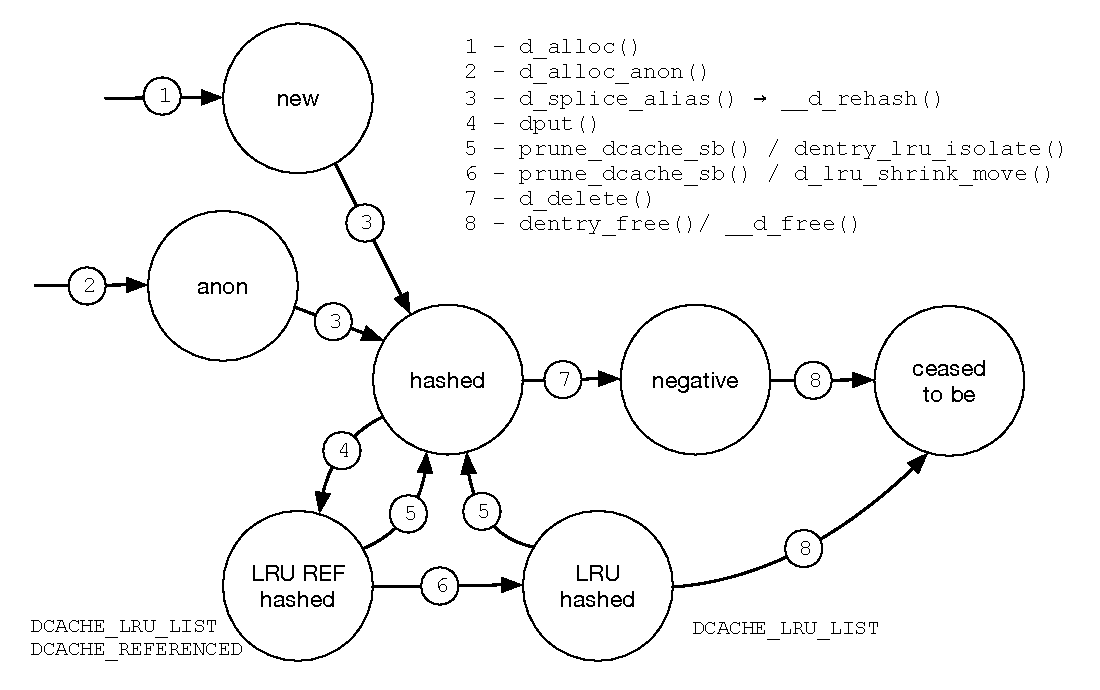
\includegraphics[scale=0.7]{figures/dcache-state.pdf}
	\centering
	\caption{The dentry state diagram}
	\label{fig:dcache-state}
\end{figure}

\textbf{XXX --- if I keep a file open (less file) will it still be on the hashed list ?}

\vspace{0.25cm}
\noindent
\textbf{Step 1}  % STEP 1

\vspace{0.25cm}
\noindent
The first way that a dentry comes into existence is with a call to \cf{d\_alloc()} which in turn calls \cf{\_\_d\_alloc()}. This calls \cf{kmem\_cache\_alloc\_lru(dentry\_cache, ...)} and initializes the fields of the \cf{dentry} structure. You will see how the name is stored (whether to use \cf{d\_iname} or \cf{d\_name} depending on the size of the file name (\cf{DNAME\_INLINE\_LEN}).

Before a return is made from \cf{d\_alloc()}, the dentry will be added to the parent's \cf{d\_subdirs} list. This list goes through the children's \cf{d\_child} field. At this point the dentry is not hashed.

\vspace{0.25cm}
\noindent
\textbf{Step 2}  % STEP 2

\vspace{0.25cm}
\noindent
The second way that a dentry comes into existence is if the parent of this new entry is not in the dcache. In this case, an \textit{anonymous dentry} will be created. This occurs is when mounting a filesystem. Since the inode for the root of the tree has no direct parent, the filesystem will read in the filesystem's root inode and call \cf{d\_make\_root()} which in turn calls \cf{d\_alloc\_anon()} to create the associated dentry. This function is typically called by the filesystem's \textit{fill\_super} function.

\vspace{0.25cm}
\noindent
\textbf{Step 3}  % STEP 3

\vspace{0.25cm}
\noindent
After a dentry is allocated, a call is typically made to the filesystem's \textit{lookup} function which locates and reads in the inode and then calls \cf{d\_splice\_alias()} to associate the dentry with the newly created inode. The filesystem's lookup function will be part of the \cf{inode\_operations} structure that the filesystem attaches to the \cf{i\_op} field of the \cf{inode} structure for a directory file type.

The following sequence of calls occurs:

\small
\bigskip 
filesystem $\rightarrow$ \cf{d\_splice\_alias()} $\rightarrow$ \cf{\_\_d\_add()}  $\rightarrow$ \cf{\_\_d\_rehash()}
%\\~\\
    
\bigskip
\normalsize
\noindent
The function \cf{\_\_d\_rehash()} adds the dentry to the appropriate hash bucket:

\begin{lstlisting}
static void 
[*\bfseries \_\_d\_rehash*](struct dentry *entry)
{  
    struct hlist_bl_head *b = [*\bfseries d\_hash*](entry->d_name.hash);

    hlist_bl_lock(b);
    [*\bfseries hlist\_bl\_add\_head\_rcu*](&entry->d_hash, b);
    hlist_bl_unlock(b);
}  
\end{lstlisting}

\noindent
This is the only function that adds a dentry to the hash table. Other callers will be described in a later section.

\vspace{0.25cm}
\noindent
\textbf{Step 4}  % STEP 4

\vspace{0.25cm}
\noindent
When a file is no longer needed to perform the particular task required, \cf{dput()} is called which decrements the dentry's reference count. If it drops to zero, it will be moved to the LRU list and may be reclaimed later if there is a memory shortage. \cf{DCACHE\_LRU\_LIST} is added to \cf{d\_flags} to show that the dentry is on the LRU list. A call is also made to \cf{retain\_dentry()} to see if the dentry should be retained. If this is the case, the \cf{DCACHE\_REFERENCED} flag will also be set in \cf{d\_flags}.

\begin{lstlisting}
static void 
[*\bfseries d\_lru\_add*](struct dentry *dentry)
{   
    dentry->d_flags |= DCACHE_LRU_LIST;
    [*\bfseries list\_lru\_add*](&dentry->d_sb->s_dentry_lru, &dentry->d_lru);
}    
\end{lstlisting}

\noindent
Why might the \cf{DCACHE\_REFERENCED} flag not be set? See the \cf{retain\_dentry()} for details but there are four conditions under which this could occur including the case where \cf{DCACHE\_DONTCACHE} is set or if the dentry is disconnected. \textbf{XXX -- really need to read through \cf{fast\_dput()} and see why it's setting these flags. most work is done in there}

\cf{d\_lru\_add()} also called by \cf{dentry\_kill()} and \cf{dput\_to\_list()}. They will be described in more detail later in this section.

\vspace{0.25cm}
\noindent
\textbf{Step 6}  % STEP 5

\vspace{0.25cm}
\noindent
When the per-superblock LRU list is being scanned to see if dentries can be retired to reclaim memory, if the dentry is still in use, the \cf{DCACHE\_REFERENCED} flag is turned off by \cf{dentry\_lru\_isolate()} and it returns to the simple hashed state but it taken off the LRU list. Section \ref{dcache-pruning} describes the pruning process.

\vspace{0.25cm}
\noindent
\textbf{Step 6}  % STEP 6

\vspace{0.25cm}
\noindent
If the dentry has not been accessed in quite a while and there are no references to it, the \cf{DCACHE\_REFERENCED} will be turned off in \cf{dentry\_lru\_isolate()} allowing for the dentry to be reclaimed. A call is made to \cf{d\_lru\_shrink\_move()} which turns on the \cf{DCACHE\_SHRINK\_LIST} flag and moved to the disposable list (see \cf{prune\_dcache\_sb()}). Pruning the dcache is covered in section \ref{dcache-pruning}. \textbf{XXX -- OK so need to understand this better}

\vspace{0.25cm}
\noindent
\textbf{Step 7}  % STEP 7

\vspace{0.25cm}
\noindent
When a file is unlinked a call is made to \cf{d\_delete()} to turn the dentry into a negative dentry. The path starting at the system call layer will be:

\small
\bigskip 
\cf{vfs\_unlink()} $\rightarrow$ \cf{d\_delete\_notify()} $\rightarrow$ \cf{d\_delete()}

%\\~\\
    
\bigskip
\normalsize
\noindent
and from \cf{d\_delete()} onwards:

\small
\bigskip 
\cf{d\_delete()} $\rightarrow$ \cf{dentry\_unlink\_inode()}  $\rightarrow$ \cf{\_\_d\_clear\_type\_and\_inode()}
%\\~\\
    
\bigskip
\normalsize
\noindent
The \cf{DCACHE\_ENTRY\_TYPE} and \cf{DCACHE\_FALLTHRU} flags are turned off in \cf{d\_flags} and the \cf{d\_inode} field is set to \cf{NULL}. By turning off the \cf{DCACHE\_ENTRY\_TYPE} flag, any caller trying to determine the type of the file from the dentry will not get a valid response back from \cf{\_\_d\_entry\_type()}.

\vspace{0.25cm}
\noindent
\textbf{Step 8}  % STEP 8

\vspace{0.25cm}
\noindent
The last phase in the lifecycle of a dentry involves a call to \cf{dentry\_free()}. This can be from one of several functions namely \cf{dentry\_kill()}, \cf{d\_prune\_aliases()}, \cf{shrink\_dentry\_list()} or \cf{shrink\_dcache\_parent()}

\cf{dentry\_free()}  calls t\cf{\_\_d\_free()} which calls \cf{kmem\_cache\_free()} to free the \cf{dentry} structure. There may also be a call to \cf{\_\_d\_free\_external()} for dentries that needed external space allocated for a longer filename. 

%-----------------------------------------------------------------------------------------------------------------------------------------------------------------

\subsection{KGDB -- Monitoring dentry Transition State}

One of the hardest aspects of understanding the dcache for me was the transition between different states. I followed an old Linux Journal article that gave a state diagram but the article was almost twenty years old and some functions didn't exist. Recreating that state diagram with a newer Linux kernel wasn't easy and took a lot of sessions in \cf{gdb} in conjunction with similar sessions for pathname resolution. And this is why being able to analyze the kernel when running and setting breakpoints is imperative to understanding how the kernel works.

This example takes a simple command and shows the file's dentry after pathname resolution is complete to show that it should be on both hashed and LRU lists. This is the command that we'll use which keeps the file open:

\begin{lstlisting}
$ [*\bfseries less lorem-ipsum *]
\end{lstlisting}

\noindent
The first step is to set a breakpoint in \cf{do\_filp\_open()} so that we can locate the dentry returned for "\cf{lorem-ipsum}":

\begin{lstlisting}
(gdb) [*\bfseries br do\_filp\_open if \$\_streq(pathname->name, "lorem-ipsum")*]
Breakpoint 26 at 0xffffffff813fe8c0: file fs/namei.c, line 3678.
\end{lstlisting}

\noindent
When running the command, we hit the breakpoint and step through \cf{do\_filp\_open()} until we see a return from \cf{path\_openat()}:

\begin{lstlisting}
Thread 2 hit Breakpoint 26, do_filp_open (dfd=dfd@entry=-100, 
pathname=pathname@entry=0xffff8881009a2000, 
op=op@entry=0xffffc900014dbebc) at fs/namei.c:3678
3678	{
(gdb) [*\bfseries n*]
3679		struct nameidata nd;
(gdb) [*\bfseries  n*]
3683		set_nameidata(&nd, dfd, pathname, NULL);
(gdb) [*\bfseries 
610		p->state = 0;
(gdb) [*\bfseries  n*]
3683		set_nameidata(&nd, dfd, pathname, NULL);
(gdb) [*\bfseries  n*]
3684		filp = path_openat(&nd, op, flags | LOOKUP_RCU);
(gdb) [*\bfseries  n*]
3685		if (unlikely(filp == ERR_PTR(-ECHILD)))
\end{lstlisting}

\noindent
One return from \cf{path\_openat()} we can look at the \cf{file} structure and check that we have the right file:

\begin{lstlisting}
(gdb) [*\bfseries  p filp->f\_path*]
$225 = {
  mnt = 0xffff88812ecffba0,
  dentry = 0xffff8881032cd0c0
}
(gdb) [*\bfseries  p filp->f\_path->dentry->d\_iname*]
$226 = "lorem-ipsum", '\000' <repeats 20 times>
\end{lstlisting}

\noindent
and from the \cf{file} structure we can also access the dentry for the file and look at the flags:

\begin{lstlisting}
(gdb) [*\bfseries  p/x filp->f\_path->dentry->d\_flags*]
$231 = 0x480040
\end{lstlisting}

\noindent
Here are the values for the \cf{d\_flags} field:

\begin{lstlisting}
#define DCACHE_REGULAR_TYPE   0x00400000 /* Regular file type */
#define DCACHE_LRU_LIST       0x00080000
#define DCACHE_REFERENCED     0x00000040 /* Recently used, 
                                            don't discard. */
\end{lstlisting}

\noindent
We can also check the hash list and LRU list. The dentry should be on both lists according to the flags:

\begin{lstlisting}
(gdb) [*\bfseries  p filp->f\_path->dentry->d\_hash*]
$232 = {
  next = 0x0 <fixed_percpu_data>,
  pprev = 0xffff88817b975948
}
(gdb) [*\bfseries  p filp->f\_path->dentry->d\_lru*]
$233 = {
  next = 0xffff8881032cdb00,
  prev = 0xffff888103050c80
}
\end{lstlisting}

\noindent
It is indeed on both lists as expected. Since it's hashed, if we access the file again, the dentry will be found quickly. Note that the hold on the dentry is dropped once pathname resolution is complete even though we still have the file open (due to running \cf{less(1)}).

%-----------------------------------------------------------------------------------------------------------------------------------------------------------------

\subsection{Digging Deeper on The Core Functions}

With the state diagram in mind, the following sections dig deeper on the internal operations of the dcache.

Here are the main functions ... there is a mismatch between the above diagram and this list. i know I am using d\_splice\_alias()


%%%%%%%%%%%%%%%%%%

Expand on the basics so I really understand them. Will help with the state diagram.

Pruning the dcache is covered in section \ref{dcache-pruning}.

% d_alloc()

\subsubsection{\cf{d\_alloc()}}

Callers of \cf{d\_alloc()} will get back a new dentry with this new dentry linked on the \cf{d\_subdirs} list of the parent but the dentry will not be on the hash queue at this point. 

Here are the main paths through \cf{d\_alloc()}: \textbf{XXX -- come back to described locking}

\begin{lstlisting}
struct dentry *
[*\bfseries d\_alloc*](struct dentry * parent, const struct qstr *name)
{   
    struct dentry *dentry = [*\bfseries \_\_d\_alloc*](parent->d_sb, name);
    spin_lock(&parent->d_lock);
    [*\bfseries \_\_dget\_dlock*](parent);
    dentry->d_parent = parent;
    [*\bfseries list\_add*](&dentry->d_child, &parent->d_subdirs);
    spin_unlock(&parent->d_lock);
    return dentry;
}   
\end{lstlisting}

\noindent
An empty dentry is returned by \cf{\_\_d\_alloc()}, a lock is taken on the parent dentry while this new entry is added to the \cf{d\_subdirs} field. On return from \cf{d\_alloc()}, there is no associated inode. Much of the code in \cf{\_\_d\_alloc()} deals with allocation and initialization of the different fields in the \cf{dentry} structure:

% __d_alloc()

\begin{lstlisting}
static struct dentry *
[*\bfseries \_\_d\_alloc*](struct super_block *sb, const struct qstr *name)
{
    struct dentry *dentry;
    char *dname;
        
    dentry = [*\bfseries kmem\_cache\_alloc\_lru*](dentry_cache, 
                               &sb->s_dentry_lru, GFP_KERNEL);
    dentry->d_iname[DNAME_INLINE_LEN-1] = 0;
    ...
    } else if (name->len > DNAME_INLINE_LEN-1) {
        /* kmalloc() space for the name */
        *p = [*\bfseries kmalloc*](...);
        dname = p->name;
    } else  {
        dname = dentry->d_iname;
    }
   
    dentry->d_name.len = name->len;
    dentry->d_name.hash = name->hash;
    memcpy(dname, name->name, name->len);

    dentry->d_inode = NULL;
    dentry->d_parent = dentry;
    dentry->d_sb = sb;
    INIT_HLIST_BL_NODE(&dentry->d_hash);
    INIT_LIST_HEAD(&dentry->d_lru);
    INIT_LIST_HEAD(&dentry->d_subdirs);
    INIT_HLIST_NODE(&dentry->d_u.d_alias);
    INIT_LIST_HEAD(&dentry->d_child);

    return dentry;
}
\end{lstlisting}

\noindent
If the length of the filename is small enough, it's copied to \cf{d\_iname} otherwise memory is allocated and it will be copied to \cf{d\_name.name}. All lists are initialized but at this stage, the dentry is only added to \cf{d\_subdirs} when a return is made to \cf{d\_alloc()}.

Callers of \cf{d\_alloc()} are shown on the left-hand side of figure \ref{fig:d-alloc}.

\begin{figure}[h]
	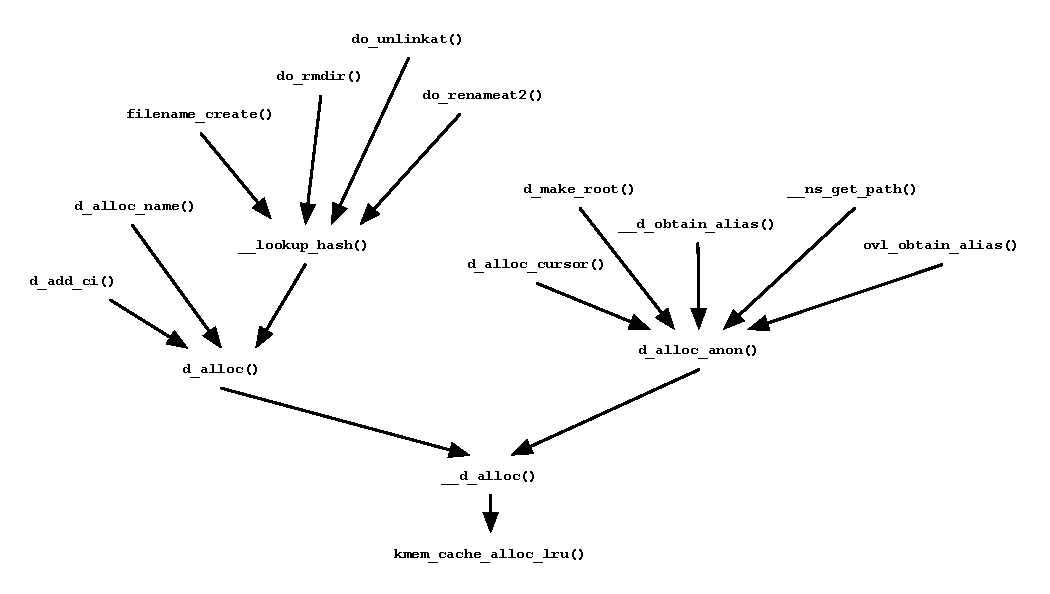
\includegraphics[scale=0.7]{figures/d-alloc.pdf}
	\centering
	\caption{Callers of \cf{d\_alloc()}}
	\label{fig:d-alloc}
\end{figure}

\noindent
The function \cf{d\_add\_ci()} is called to lookup or allocate a new dentry with case-exact name. The only callers are the NTFS and XFS filesystems. By default, NTFS is case-insensitive (although that can be disabled during mount). XFS provides an option for filenames to be case-insensitive. All other Linux filesystems are case-sensitive so "\cf{filename}" and "\cf{FILENAME}" are both valid files in the same directory.

The \cf{d\_alloc\_name()} function is called by procfs, configfs, SELinux and others. Sometimes it is to create a dentry for the root inode and in the case of procfs, one use is to set up \cf{/proc/self}.

Callers of \cf{filename\_create()} are shown in figure \ref{fig:link-path-walk-callers} but include creation of symlinks, hard links and device nodes. Along with the other functions shown, it calls \cf{\_\_lookup\_hash()} which will call the \cf{lookup} operation 

\subsubsection{\cf{d\_alloc\_anon()}}

Shown on the right-hand side of figure \ref{fig:d-alloc}, \cf{d\_alloc\_anon()} simply makes a call is made to \cf{\_\_d\_alloc()} as follows:

\begin{lstlisting}
struct dentry *
[*\bfseries d\_alloc\_anon*](struct super_block *sb)
{
    return [*\bfseries \_\_d\_alloc*](sb, NULL);
}
\end{lstlisting}

\noindent
There is no \cf{name} field passed as an so \cf{NULL} is passed to \cf{\_\_d\_alloc()} and on return, there is no parent to associated this new dentry with (thus an anonymous dentry). Non of the initialization described above applies to anonymous dentries.

There are several callers of \cf{d\_alloc\_anon()} but the most common case occurs when mounting a filesystem. When the filesystem \textit{fill\_super} function is called, it reads in the root inode and calls \cf{d\_make\_root()} which in turn calls \cf{d\_alloc\_anon()}.

% retain_dentry() / d_put()

\subsubsection{\cf{retain\_dentry()} and \cf{d\_put}}

Each mounted filesystem has an LRU list hanging off the \cf{} field of the \cf{super\_block} structure. This makes a lot of sense. When a filesystem is unmounted, walking the list of dentries needs to be efficient. 

In the original state diagram referenced earlier in this chapter, dentries were moved from the pure \textit{hashed} state and added to the LRU list through a call to \cf{dput()}. Today, there are multiple callers and it's actually \cf{retain\_dentry()} which is the only function to call \cf{d\_lru\_add} to add a dentry to the LRU list. The overall paths to this function are shown in figure \ref{fig:dentry-lru-add}. Note that the \cf{DCACHE\_LRU\_LIST} flag is set by \cf{d\_lru\_add} and on return, \cf{DCACHE\_REFERENCED} is set by \cf{retain\_dentry()} if it is not already set by another thread.

\begin{figure}[h]
	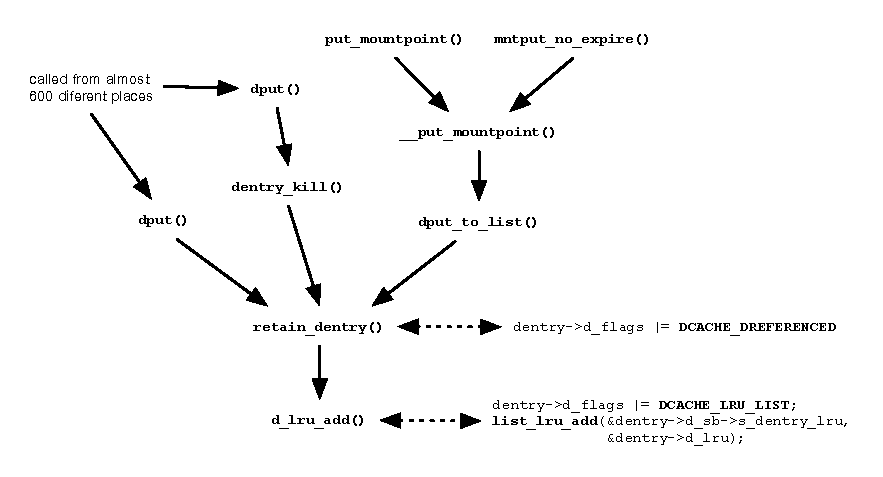
\includegraphics[scale=0.8]{figures/dentry-lru-add.pdf}
	\centering
	\caption{Adding a dentry to the superblock LRU list}
	\label{fig:dentry-lru-add}
\end{figure}

You will notice that there are two paths going thrrough \cf{dput()}. The first path involves calling \cf{retain\_dentry()} directly and the second passes through \cf{dentry\_kill()}. Here is the code to \cf{dput()}:

\begin{lstlisting}
void 
[*\bfseries dput*](struct dentry *dentry)
{
        if (likely([*\bfseries fast\_dput*](dentry))) {
            return;
        }
        if (likely([*\bfseries retain\_dentry*](dentry))) {
            return;
        }
        dentry = [*\bfseries dentry\_kill*](dentry);
    }
}
\end{lstlisting}

\noindent
A call is made to \cf{fast\_dput()} to perform a \textit{lockless} \cf{dput()}. \textbf{XXX --- need to look through this code}

In almost all circumstances, the dentry will be moved to the LRU list. There are checks inside \cf{retain\_dentry()} which specify that the dentry should no longer be kept and \textbf{XXX --- need to explain some of these at least}. 

% d_splice_alias() / d\_instantiate()

\subsubsection{\cf{d\_splice\_alias} and \cf{d\_instantiate()}}

\cf{d\_splice\_alias()} is called during lookup where it will instantiate the dentry if the file is found otherwise it will instantiate a negative dentry. As the comment at the top of the function states that this function will "\textit{splice a disconnected dentry into the tree if one exists}". This function calls \cf{\_\_d\_add()} which in turn calls \cf{\_\_d\_set\_inode\_and\_type()} to set the \cf{d\_inode} field to point to the inode and initialize \cf{d\_flags}. It also calls \cf{\_\_d\_rehash()} which will add the dentry to the correct hash bucket. The callers of are shown in figure \ref{fig:d-splice-alias}.

\begin{figure}[h]
	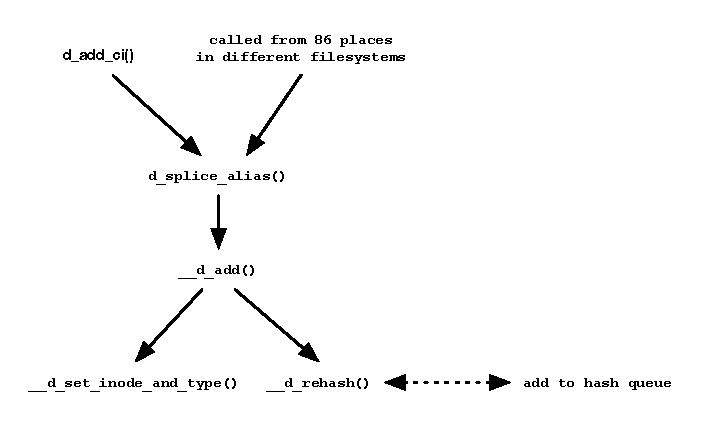
\includegraphics[scale=0.8]{figures/d-splice-alias.pdf}
	\centering
	\caption{Using \cf{d\_splice\_alias()} to add an inode to a negative dentry}
	\label{fig:d-splice-alias}
\end{figure}

\cf{d\_instantiate()} is called by the filesystem during a creation type event such as "create", "mkdir", "symlink" and "link". In all of these cases a dentry is passed as an argument. For example, take a call into SPFS for directory creation:

\begin{lstlisting}
sp_mkdir(struct user_namespace *mnt_userns, struct inode *dip,
         struct dentry *dentry, umode_t mode)
\end{lstlisting}

\noindent
In all of these functions a call to the filesystem's \textit{lookup} function will have been called which will have previously instantiated a negative dentry.

\begin{figure}[h]
	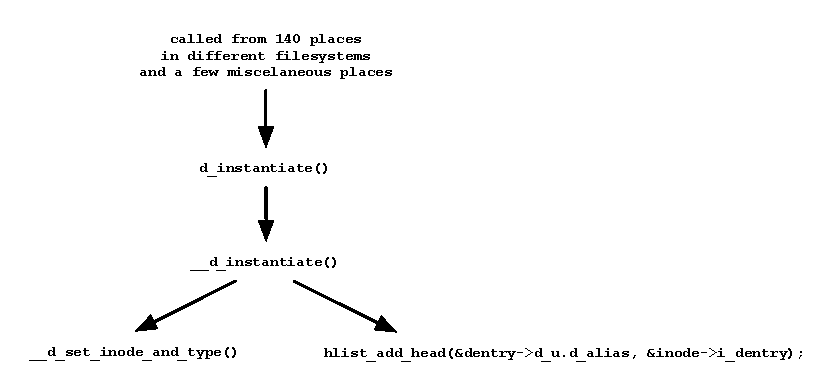
\includegraphics[scale=0.8]{figures/d-instantiate.pdf}
	\centering
	\caption{Callers of \cf{d\_instantiate()} which are passed a negative dentry}
	\label{fig:d-instantiate}
\end{figure}

\noindent
\textbf{The "i\_count" member in the inode structure should be set/incremented. I don't cover this anywhere}

% d_add() - who the hell calls this???

\subsubsection{\cf{d\_add()}}

This function is called to get a hold on the dentry to ensure that it stays in the cache while some other operation is performed like \textbf{XXX}.

\begin{lstlisting}
static inline struct dentry *
[*\bfseries dget*](struct dentry *dentry)
{
    if (dentry)
        [*\bfseries lockref\_get*](&dentry->d_lockref);
    return dentry;
}
\end{lstlisting}

\noindent
The \cf{d\_lockref} uses the lockref primitive to provide both a spinlock and a reference count. Inside \cf{lockref\_get()}, the spinlock is taken and the reference count is incremented:

\begin{lstlisting}
spin_lock(&lockref->lock);
lockref->count++;
spin_unlock(&lockref->lock);
\end{lstlisting}

\noindent
xxx

% d_delete()

\subsubsection{\cf{d\_delete}}

TBD

\subsubsection{\cf{d\_delete}}

delete a dentry. If there are no other open references to the dentry then the dentry is turned into a negative dentry (the d\_iput() method is called). If there are other references, then d\_drop() is called instead

\subsubsection{\cf{dget}}

open a new handle for an existing dentry (this just increments the usage count)

\subsubsection{\cf{dput}}

close a handle for a dentry (decrements the usage count). If the usage count drops to 0, and  the dentry is still in its parent's hash, the "d\_delete" method is called to check whether it should be cached. If it  should not be cached, or if the dentry is not hashed, it is deleted. Otherwise cached dentries are put into an LRU list to be reclaimed on memory shortage.
		
\subsubsection{\cf{d\_drop}}

this unhashes a dentry from its parents hash list. A subsequent call to dput() will deallocate the dentry if its usage count drops to 0
		
\subsubsection{\cf{d\_add}}

add  a dentry to its parents hash list and then calls d\_instantiate()

%-----------------------------------------------------------------------------------------------------------------------------------------------------------------

\subsection{Pruning The Dcache}\label{dcache-pruning}

To help with putting the state diagram together, a key piece of the puzzle is to look at when \cf{DCACHE\_REFERENCED} was turned on and off in \cf{d\_flags}. 

As described earlier in this section and shown in figure \ref{fig:dentry-lru-add} the only place where the \cf{DCACHE\_REFERENCED} is set is inside \cf{retain\_dentry()} which is generally called through the \cf{dput()} path.

Similarly, the flag is only turned off in \cf{dentry\_lru\_isolate()} and this function is only called by \cf{prune\_dcache\_sb()} which is shown in figure \ref{fig:dcache-prune}. in turn is only called by \cf{super\_cache\_scan()} which will be discussed in the next section.

At some point, the dentry will have the  \cf{DCACHE\_REFERENCED} flag removed and be a candidate for deletion. Refer to figure \ref{fig:dcache-prune}. The \cf{super\_cache\_scan()} function is assigned to the \cf{s\_shrink.scan\_objects} field of the \cf{super\_block} during a call from \cf{alloc\_super()}. This occurs when a filesystem is being mounted. This function will run \textbf{XXX - when does it run?}

\begin{figure}[h]
	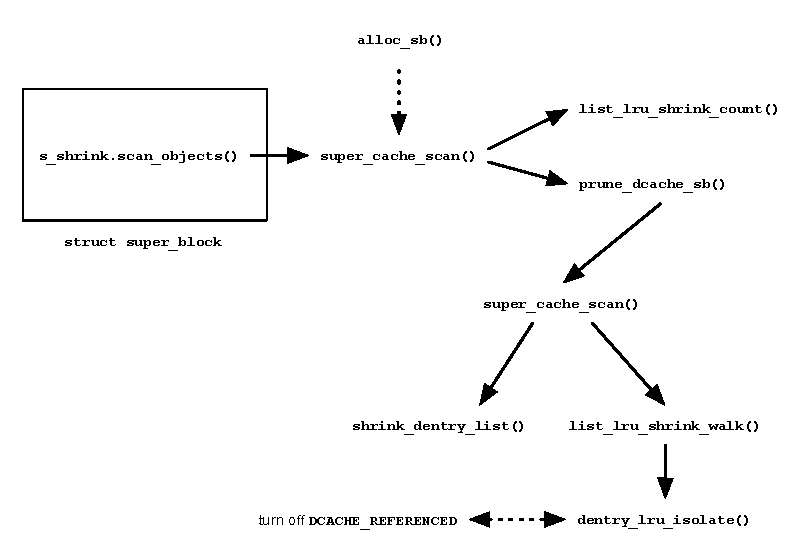
\includegraphics[scale=0.7]{figures/dcache-prune.pdf}
	\centering
	\caption{Pruning dcache entries for a specific filesystem}
	\label{fig:dcache-prune}
\end{figure}

\noindent
Inside \cf{super\_cache\_scan()}, a call is made to \cf{prune\_dcache\_sb()} which processes the LRU list eventually calling \cf{dentry\_lru\_isolate()}. This turns off the \cf{DCACHE\_REFERENCED} flag and \textbf{XXX} allows for the dentry to deleted.

%-----------------------------------------------------------------------------------------------------------------------------------------------------------------

\subsection{KGDB -- Analyzing Dentries For a Simple File Hierarchy}

This example will show how dentries are connected together for a filesystem with a small number of files and directories which is mounted on \cf{/mnt}. We have the following files and since we're accessing them all, they will have been brought into the dcache.

\begin{lstlisting}
$ [*\bfseries find /mnt*]
/mnt
/mnt/lost+found
/mnt/mydir
/mnt/mydir/lorem-ipsum
/mnt/mydir/hello
\end{lstlisting}

\noindent
Let's get the root dentry for our mounted filesystem. I know it was the last filesystem mounted so I just use the \cf{prev} pointer when displaying the \cf{super\_blocks} list. This address is assigned to the convenience variable \cf{\$sb} and the \cf{s\_root} field is displayed. This points to the root dentry for this filesystem. The address is saved in the convenience variable \cf{\$rd}.

\begin{lstlisting}
(gdb) [*\bfseries p super\_blocks*]
$136 = {
  next = 0xffff88810005a800,
  prev = 0xffff88810cc90800
}
(gdb) [*\bfseries set \$sb = (struct super\_block *)0xffff88810cc90800*]
(gdb) [*\bfseries pipe p *\$sb | grep s\_root*]
  s_root = 0xffff888101cc7540,
(gdb) [*\bfseries set \$rd = (struct dentry *)0xffff888101cc7540*]
\end{lstlisting}

\noindent
As a sanity check we look to see that its parent is the same address (the root of a filesystem) and that the name is "/".

\begin{lstlisting}
(gdb) [*\bfseries p \$rd->d\_parent*]
$142 = (struct dentry *) 0xffff888101cc7540
(gdb) [*\bfseries p *\$rd->d\_iname*]
$141 = 47 '/'
\end{lstlisting}

\noindent
Now let's look at the \cf{d\_flags} field for this root dentry:

\begin{lstlisting}
(gdb) [*\bfseries p/x \$rd->d\_flags*]
$144 = 0x200000
\end{lstlisting}

\noindent
Here is the type (\cf{dcache.h}). This is the only flag set.

\noindent
\begin{lstlisting}
DCACHE_DIRECTORY_TYPE    0x00200000 /* Normal directory */
\end{lstlisting}

\noindent
The next step is to look at the \cf{d\_subdirs} field which points to a doubly linked list of children that are in the dcache:

\begin{lstlisting}
(gdb) [*\bfseries p \$rd->d\_subdirs*]
$145 = {
  next = 0xffff888102eb3e10,
  prev = 0xffff888102eb1a50
}
\end{lstlisting}

\noindent
This list goes through the \cf{d\_child} field of the \cf{dentry} structure so we need to call \cf{container\_of()} to get the correct address of each structure:

\begin{lstlisting}
(gdb) [*\bfseries set \$c1 = \$container\_of(0xffff888102eb3e10, \textbackslash*]
                                    [*\bfseries "struct dentry", "d\_child")*]
(gdb) [*\bfseries set \$c2 = \$container\_of(0xffff888102eb1a50,  \textbackslash*]
                                    [*\bfseries "struct dentry", "d\_child")*]
\end{lstlisting}

\noindent
From here, we can check the the filenames:

\begin{lstlisting}
(gdb) [*\bfseries p \$c1->d\_iname*]
$152 = "lost+found", '\000' <repeats 21 times>
(gdb) [*\bfseries p \$c2->d\_iname*]
$153 = "mydir", '\000' <repeats 26 times>
\end{lstlisting}

\noindent
and then the \cf{d\_flags} field of each dentry:

\begin{lstlisting}
(gdb) [*\bfseries p/x \$c1->d\_flags*]
$155 = 0x280040
(gdb) [*\bfseries p/x \$c2->d\_flags*]
$156 = 0x280040
\end{lstlisting}

\noindent
Breaking down \cf{d\_flags} (\cf{dcache.h}) shows that the following flags are set:

\begin{lstlisting}
DCACHE_LRU_LIST        0x00080000 /* dentry is on the LRU list*/
DCACHE_REFERENCED      0x00000040 /* Recently used, 
                                     don't discard. */
DCACHE_DIRECTORY_TYPE  0x00200000 /* Normal directory */
\end{lstlisting}

\noindent
Now let's look at the child files:

\begin{lstlisting}
(gdb) [*\bfseries p \$c2->d\_subdirs*]
$183 = {
  next = 0xffff888103050bd0,
  prev = 0xffff8881030502d0
}
(gdb) [*\bfseries set \$f1 = \$container\_of(0xffff888103050bd0, \textbackslash*]
                               [*\bfseries "struct dentry", "d\_child")*]
(gdb) [*\bfseries set \$f2 = \$container\_of(0xffff8881030502d0, \textbackslash*]
                               [*\bfseries "struct dentry", "d\_child")*]
\end{lstlisting}

\begin{lstlisting}
(gdb) [*\bfseries p \$f1->d\_iname*]
$160 = "hello", '\000' <repeats 26 times>
(gdb) [*\bfseries p \$f2->d\_iname*]
$162 = "lorem-ipsum", '\000' <repeats 20 times>
\end{lstlisting}

\noindent
and the contents of \cf{d\_flags} for each dentry:

\begin{lstlisting}
(gdb) [*\bfseries p/x \$f1->d\_flags*]
$164 = 0x480040
(gdb) [*\bfseries p/x \$f2->d\_flags*]
$163 = 0x480040
\end{lstlisting}

\noindent
Breaking down \cf{d\_flags} (\cf{dcache.h}) shows that the following flags are set:

\begin{lstlisting}
DCACHE_LRU_LIST      0x00080000
DCACHE_REFERENCED    0x00000040 /* Recently used, 
                                   don't discard. */
DCACHE_REGULAR_TYPE  0x00400000 /* Regular file type  */
\end{lstlisting}

\noindent
The \cf{mydir} directory and both of the files \cf{lorem-ipsum} and \cf{hello} have both the \cf{DCACHE\_LRU\_LIST} and \cf{DCACHE\_REFERENCED} flags set indicating that they are on the LRU list although there are no holds on the dentries at this point. 

%-----------------------------------------------------------------------------------------------------------------------------------------------------------------

\subsection{KGDB -- Inspecting the Per-Filesystem LRU List}

could be combined with above. need to rerun the example. i lost the fs somehow.

\textbf{XXX - small FS - look at everything on there - need to come back to this. harder than I thought. Can't find the right stuff}

\begin{lstlisting}
$ [*\bfseries find /mnt*]
/mnt
/mnt/lost+found
/mnt/lorem-ipsum
/mnt/mydir
/mnt/mydir/myfile
\end{lstlisting}

\noindent
xxx

\begin{lstlisting}
(gdb) [*\bfseries p super\_blocks*]
$16 = {
  next = 0xffff88810005a800,
  prev = 0xffff8881216de800
}
(gdb) [*\bfseries set \$sb = (struct super\_block *)0xffff8881216de800*]
\end{lstlisting}

\noindent
xxx

\begin{lstlisting}
struct list_lru_node {
    spinlock_t      lock;
    struct list_lru_one lru;
    long            nr_items;
};

struct list_lru {
    struct list_lru_node    *node;
#ifdef CONFIG_MEMCG_KMEM
    struct list_head    list;
    int         shrinker_id;
    bool            memcg_aware;
    struct xarray       xa;
#endif
};
\end{lstlisting}

\noindent
xxx

%-----------------------------------------------------------------------------------------------------------------------------------------------------------------

\subsection{Dcache Statistics}

The dcache exports informaiton through the following /proc interface:

\begin{lstlisting}
$ [*\bfseries cat /proc/sys/fs/dentry-state*]
159548	137775	45	0	48194	0
\end{lstlisting}

\noindent
These entries correspond to the following structure defined in \cf{fs/dcache.c}:

\begin{lstlisting}
struct dentry_stat_t { 
    long nr_dentry;
    long nr_unused;
    long age_limit;     /* age in seconds */
    long want_pages;    /* pages requested by system */
    long nr_negative;   /* # of unused negative dentries */
    long dummy;         /* Reserved for future use */
};  
\end{lstlisting}

\noindent
The routines for providing this information can also be found in the same file. If you look throughout the various dcache functions you will see calls to \cf{this\_cpu\_inc()} and \cf{this\_cpu\_dec()} which increment and decrement the number of entries used.

\textbf{Come back here near the end to see if newer OS versions have picked up any changes}

%%%%%%%%%%%%%%%%%%%%%%%%%%%%%%%%%%%%%%%%%%%%%%%%%%%%%%%%%%%%%%%

\section{The Inode Cache Implementation}\label{vfs-inode-cache}

TBD

\textbf{XXX -- Need to cover the list fields in the kern-structs chapter}

Look at % https://www.cs.kent.edu/~bennett/class/kernel/sum99/notes/wk8/mount.html

%---------------------------------------------------------------------------------------------------------------------------------------------------------------------

\subsection{Inode Locks}

% VFS 2020.pdf has a lot of info

\textbf{XXX -- Not sure that this is the correct place. Perhaps later in VFS?}

\begin{itemize}
	\item \cf{i\_rwsem} -- a read/write semaphore that serializes changes to a directory. It's also involved in pathname 
		resolution re: looking at the dcache \textbf{XXX -- need to come back and do this once I have a better 
		handle on things}
	\item \cf{i\_lock} -- TBD
	\item \cf{i\_mutex} -- TBD
\end{itemize}

\noindent
TBD

%%%%%%%%%%%%%%%%%%%%%%%%%%%%%%%%%%%%%%%%%%%%%%%%%%%%%%%%%%%%%%%

\section{The Buffer Cache Implementation}\label{vfs-buffer-cache}

TBD

%%%%%%%%%%%%%%%%%%%%%%%%%%%%%%%%%%%%%%%%%%%%%%%%%%%%%%%%%%%%%%%

\section{File Creation}

section covers the creation of regular files, directories, symlinks, hard links and device nodes and shows the reliance on pathname resolution to get to all but the last component which needs special handling based on the type of file that is being created. It is recommended to first refer to section \ref{openfile} to understand the basics of pathname resolution before reading this section.

%------------------------------------------------------------------------------------------------------------------------------------------------------------------------

\subsection{Regular File Creation}

The \cf{open(2)} manpage describes the five different system calls that can result in creation of a regular file. These five system calls are:

\begin{lstlisting}
int open(const char *pathname, int flags);
int open(const char *pathname, int flags, mode_t mode);

int creat(const char *pathname, mode_t mode);

int openat(int dirfd, const char *pathname, int flags);
int openat(int dirfd, const char *pathname, int flags, 
           mode_t mode);

int openat2(int dirfd, const char *pathname,
            const struct open_how *how, size_t size);
\end{lstlisting}

\noindent
Section \ref{openfile} described the flow through the kernel for opening a file. We'll show how these system calls converge when a file is being created.

Here are the system call entry points in the kernel for all functions:

\begin{lstlisting}
open.c:SYSCALL_DEFINE2([*\bfseries creat*], const char __user *, 
fhandle.c:SYSCALL_DEFINE3([*\bfseries open\_by\_handle\_at*], int, 
fhandle.c:COMPAT_SYSCALL_DEFINE3([*\bfseries open\_by\_handle\_at*], 
open.c:SYSCALL_DEFINE3([*\bfseries open*], const char __user *,
open.c:SYSCALL_DEFINE4([*\bfseries openat*], int, dfd, const char __user *,
open.c:SYSCALL_DEFINE4([*\bfseries openat2*], int, dfd, 
open.c:COMPAT_SYSCALL_DEFINE3([*\bfseries open*], const char __user *,
open.c:COMPAT_SYSCALL_DEFINE4([*\bfseries openat*], int, dfd,
\end{lstlisting}

\noindent
There is a lot of code to walkthrough before a call is made into the filesystem to create a file, mostly to do with pathname resolution. Wandering around the top-level system call handling code for the above routines will show a lot of functions called. Sometimes it's very helpful to work backwards by setting a breakpoint on a filesystem's \textit{create} function and seeing the path that the kernel gets there. Using the SPFS filesystem (described in chaper \ref{disk-fs}), a breakpoint will be set on \cf{sp\_create()} as follows:

\begin{lstlisting}
(gdb) [*\bfseries br sp\_create*]
Breakpoint 28 at 0xffffffffa0656f7f: 
                 file /home/spate/spfs/kern/sp_dir.c, line 279.
\end{lstlisting}

\noindent
and then it's simply a matter of copying a file into an SPFS filesystem:

\begin{lstlisting}
$ [*\bfseries cp lorem-ipsum /mnt*]
\end{lstlisting}

\noindent
When the breakpoint is hit, here is the stacktrace:

\begin{lstlisting}
#0  [*\bfseries sp\_create*] (mnt_userns=0xffffffff82a81240 <init_user_ns>, 
    dip=0xffff88812ff34500, dentry=0xffff8881031dad80, 
    mode=33188, excl=true) at /home/spate/spfs/kern/sp_dir.c:279
#1  [*\bfseries lookup\_open*] (op=0xffffc90001177e44, got_write=true, 
    file=0xffff8881333c2500, nd=0xffffc90001177d20) 
    at fs/namei.c:3376
#2  [*\bfseries open\_last\_lookups*] (op=0xffffc90001177e44, 
    file=0xffff8881333c2500, nd=0xffffc90001177d20) 
    at fs/namei.c:3446
#3  [*\bfseries path\_openat*] (nd=nd@entry=0xffffc90001177d20, 
    op=op@entry=0xffffc90001177e44, flags=flags@entry=64) 
    at fs/namei.c:3654
#4  [*\bfseries do\_filp\_open*] (dfd=dfd@entry=-100, 
    pathname=pathname@entry=0xffff88810087d000, 
    op=op@entry=0xffffc90001177e44) at fs/namei.c:3684
#5  [*\bfseries do\_sys\_openat2*] (dfd=-100, filename=<optimized out>, 
    how=how@entry=0xffffc90001177e88) at fs/open.c:1275
#6  [*\bfseries do\_sys\_open*] (mode=<optimized out>, 
    flags=<optimized out>, filename=<optimized out>, 
    dfd=<optimized out>) at fs/open.c:1291
\end{lstlisting}

\noindent
Inside \cf{path\_open\_at()}, there is a call to \cf{open\_last\_lookups()} which in turn calls \cf{lookup\_open()} which checks to see if there is a negative dentry for this file (highlighted in bold) and if this is the case, makes a call through to the filesystem's \cf{create} function to actually create the file. Note that \cf{dir\_inode} is the parent directory.

\begin{lstlisting}
static struct dentry *
[*\bfseries lookup\_open*](struct nameidata *nd, struct file *file,
                  const struct open_flags *op,
                  bool got_write)
{
    struct dentry *dir = nd->path.dentry;
    struct inode *dir_inode = dir->d_inode;

    if ([*\bfseries !dentry->d\_inode*] && (open_flag & O_CREAT)) {
        file->f_mode |= FMODE_CREATED;
        if (!dir_inode->i_op->create) {
            error = -EACCES;
            goto out_dput;
        }
        error = dir_inode->i_op->[*\bfseries create*](idmap, dir_inode, 
                                        dentry, mode, 
                                        open_flag & O_EXCL);
}
\end{lstlisting}

\noindent
The filesystem will create an inode on disk (local filesystem) and make a call to instantiate the dentry as follows:

\begin{lstlisting}
d_instantiate(dentry, inode);
\end{lstlisting}

\noindent
For more information on the steps taken by SPFS to create a file, see section \ref{spfs-create-file}.

Having gone backwards to get to this point, it's time to go back to the system call handling. For \cf{open(2)}, \cf{creat(2)} and \cf{open\_at()} there is little work done other than call through to \cf{do\_sys\_open()}. The difference between the three functions is that the directory where the file is located is specified by the caller giving the following:

\begin{lstlisting}
SYSCALL_DEFINE4([*\bfseries openat*], int, dfd, const char __user *, filename, 
                int, flags, umode_t, mode)
{ 
    return [*\bfseries do\_sys\_open*](dfd, filename, flags, mode);
}    
\end{lstlisting}

\noindent
and for open/create:

\begin{lstlisting}
return [*\bfseries do\_sys\_open*](AT_FDCWD, pathname, flags, mode);
\end{lstlisting}

\noindent
The \cf{AT\_FDCWD} informs \cf{do\_sys\_open()} to start from the current working directory. The value of \cf{AT\_FDCWD} is \cf{-100} so it can be distinguished from a valid file descriptor (which is non-negative). There is little work to do in \cf{do\_sys\_open()} other than call \cf{build\_open\_how()} and then \cf{do\_sys\_openat2()} which is the entry point for the  \cf{openat2(2)} system call. The early parts of this function is described in section \ref{openfile}.

\textbf{Good time to pause. Really need to better understand the whole phase of link\_path\_walk() avoiding the last component and how it's different with create vs plain open}

%------------------------------------------------------------------------------------------------------------------------------------------------------------------------

\subsection{Creating Directories}\label{vfs-mkdir}

There are two system calls for directory creation namely \cf{mkdir(2)} and \cf{mkdirat(2)}. The system call handlers for both are as follows:

\begin{lstlisting}
$ [*\bfseries grep SYSCALL *.c | grep mkdir*]
namei.c:SYSCALL_DEFINE3(mkdirat, int, dfd, ...
namei.c:SYSCALL_DEFINE2(mkdir, const char __user *, ...
\end{lstlisting}

\noindent
Both of these functions do little other than making a call to \cf{do\_mkdirat()} either passing \cf{AT\_FDCWD} in the case of \cf{mkdir(2)} or for \cf{mkdirat(2)} it will be the directory file descriptor passed as the first argument.

\begin{table}[h]
\begin{tabular}{ll}
\parbox[l]{0.6in}{
\includegraphics[scale=0.8]{figures/src-xref.pdf}} & \parbox[l]{4in}{\small{Directory creation handling code can be found in \cf{fs/namei.c}.}}
\end{tabular}
\end{table}

\noindent
Most of the work in directory creation involves resolving the pathname passed. A call is made to \cf{filename\_create()} which should return a negative dentry for the new directory to be created. The creation is then performed by a call to \cf{vfs\_mkdir()}.

\begin{lstlisting}
int 
[*\bfseries do\_mkdirat*](int dfd, struct filename *name, umode_t mode)
{
    struct dentry *dentry;
    struct path path;
    unsigned int lookup_flags = LOOKUP_DIRECTORY;

    dentry = [*\bfseries filename\_create*](dfd, name, &path, lookup_flags);
    error = [*\bfseries security\_path\_mkdir*](&path, dentry,
    if (!error) {
        error = [*\bfseries vfs\_mkdir*](mnt_idmap(path.mnt), 
                          path.dentry->d_inode,
                          dentry, mode);
    }
    [*\bfseries done\_path\_create*](&path, dentry);
}
\end{lstlisting}

\noindent
Inside \cf{vfs\_mkdir}, a call is made to \cf{vfs\_prepare\_mode()} to set the directory's \textit{mode} and then the filesystem \textit{mkdir} function is called passing the parent's inode and the negative dentry.

\begin{lstlisting}
int 
[*\bfseries vfs\_mkdir*](struct mnt_idmap *idmap, struct inode *dir,
          struct dentry *dentry, umode_t mode)
{   
    unsigned max_links = dir->i_sb->s_max_links;
    
    [*\bfseries may\_create*](idmap, dir, dentry);
    mode = [*\bfseries vfs\_prepare\_mode*](idmap, dir, mode, 
                            S_IRWXUGO | S_ISVTX, 0);
    [*\bfseries security\_inode\_mkdir*](dir, dentry, mode);
    
    if (max_links && dir->i_nlink >= max_links)
        return -EMLINK;
    
    dir->i_op->[*\bfseries mkdir*](idmap, dir, dentry, mode);
}
\end{lstlisting}

\noindent
Inside the filesystem, assuming the operation is successful a call to \cf{d\_instantiate()} to instantiate the dentry with the new inode that the filesystem creates. To see how SPFS handles the \textit{mkdir} call refer to section \ref{spfs-mkdir}.

Returning to \cf{filename\_creation()}. This routine that is called by several functions when new files are created, whether directories, symbolic links or hard links. If all goes well, a negative dentry will be returned by this function resulting in a call to the filesystem to perform the appropriate create function. Much of what happens within \cf{filename\_creation()} is handling pathname resolution as the following fragment of the function shows:

\begin{lstlisting}
static struct dentry *
[*\bfseries filename\_create*](int dfd, struct filename *name,
                      struct path *path, unsigned 
                      int lookup_flags)
{    
    ....   
    error = [*\bfseries filename\_parentat*](dfd, name, reval_flag, path, 
                              &last, &type);
    if (last.name[last.len] && !want_dir)
        create_flags = 0;
    dentry = [*\bfseries \_\_lookup\_hash*](&last, path->dentry, 
                           reval_flag | create_flags);
    if ([*\bfseries d\_is\_positive*](dentry))
        goto fail;
        
    return dentry;

fail:
    [*\bfseries dput*](dentry);
    dentry = ERR_PTR(error);
    ...
    return dentry;
}
\end{lstlisting}

\noindent
There will be a call sequence as follows:

\small
\bigskip 
\cf{filename\_parentat()} $\rightarrow$ \cf{path\_parentat()}  $\rightarrow$ \cf{link\_path\_walk()}
%\\~\\
    
\bigskip
\normalsize
\noindent
This will resolve all but the last component for which a call to \cf{\_\_lookup\_hash()} is made to see if the file being created is in the dcache. We should only find a negative dentry if a new file is to be created and thus the check for \cf{d\_is\_positive()}.

%------------------------------------------------------------------------------------------------------------------------------------------------------------------------
%------------------------------------------------------------------------------------------------------------------------------------------------------------------------

\subsection{Creating Symbolic Links}\label{vfs-symlink}

There are two system calls for creation of symbolic links namely \cf{symlink(2)} and \cf{symlinkat(2)}. The system call handlers for both can be found in the \cf{fs} directory as follows:

\begin{lstlisting}
$ [*\bfseries grep SYSCALL *.c | grep symlink*]
namei.c:SYSCALL_DEFINE3(symlinkat, const char __user *, ...
namei.c:SYSCALL_DEFINE2(symlink, const char __user *, ...
\end{lstlisting}

\noindent
For \cf{symlink()} the code is very simple:

\begin{lstlisting}
    return [*\bfseries do\_symlinkat*](getname(oldname), AT_FDCWD, 
                        getname(newname));
\end{lstlisting}

\noindent
Inside \cf{do\_symlinkat()}, the path followed is very similar to that of \cf{do\_mkdirat()} as described in section \ref{vfs-mkdir}:

\begin{lstlisting}
int 
[*\bfseries do\_symlinkat*](struct filename *from, int newdfd, 
             struct filename *to)
{                 
    unsigned int lookup_flags = 0;     
    ...
    dentry = [*\bfseries filename\_create*](newdfd, to, &path, lookup_flags);
    error = [*\bfseries security\_path\_symlink*](&path, dentry, from->name);
    if (!error)
        error = [*\bfseries vfs\_symlink*](mnt_idmap(path.mnt), 
                            path.dentry->d_inode,
                            dentry, from->name);
    [*\bfseries done\_path\_create*](&path, dentry);
    ...
}
\end{lstlisting}

\noindent
Other than check permissions, \cf{vfs\_symlink()} calls in to the filesystem to create the symlink passing the parent inode and a negative dentry for the symlink file:

\begin{lstlisting}
error = dir->i_op->[*\bfseries symlink*](idmap, dir, dentry, oldname);
\end{lstlisting}

\noindent
Section \ref{diskfs-links} describes the filesystem handling side of this operation.

%------------------------------------------------------------------------------------------------------------------------------------------------------------------------
%------------------------------------------------------------------------------------------------------------------------------------------------------------------------

\subsection{Creating Hard Links and Device Nodes}

See the previous two sections for directory and symbolic link creation. For hard links, the process followed is nearly identical with the following call sequence:

\small
\bigskip 
\cf{link()} $\rightarrow$ \cf{do\_linkat()}  $\rightarrow$ \cf{filename\_lookup()} 

\vspace{1pt}
\hspace{1.50in}$\rightarrow$ \cf{vfs\_link()} $\rightarrow$ \cf{dir->i\_op->link()}
%\\~\\
    
\bigskip
\normalsize
\noindent
Where to start depends on whether \cf{link(2)} or \cf{linkat(2)} is called. 

For hard links, the process is the same as follows:

\small
\bigskip 
\cf{mknod()} $\rightarrow$ \cf{do\_mknodat()}  $\rightarrow$ \cf{filename\_lookup()} 

\vspace{1pt}
\hspace{1.65in}$\rightarrow$ \cf{vfs\_mknod()} $\rightarrow$ \cf{dir->i\_op->mknod()}
%\\~\\
    
\bigskip
\normalsize
\noindent
For all functions, see \cf{fs/namei.c} for details.

%%%%%%%%%%%%%%%%%%%%%%%%%%%%%%%%%%%%%%%%%%%%%%%%%%%%%%%%%%%%%%%
%%%%%%%%%%%%%%%%%%%%%%%%%%%%%%%%%%%%%%%%%%%%%%%%%%%%%%%%%%%%%%%

\section{Reading Directory Entries}\label{vfs_readdir}

The first time I came across the term \textit{cookies} was over thirty years ago and in conjunction with how the kernel handled reading directory entries. User programs don't necessarily know how many entries there are so they allocate a fixed size buffer and make repeated calls into the kernel. The kernel kept track of where the application was so that it could start from the place it stopped on the previous call.

Like pathname resolution, reading directory entries can be a little messy to follow. \textbf{is it-come back to be sure}.

Section \ref{prog-readdir} described the user-level interfaces for reading directory entries and mentioned the \cf{getdents(2)} system call. In the manpage it instructs users not to use the system call interfaces directory but to look at the \cf{readdir(3)} manpage for the POSIX-conforming C library interface.

\begin{table}[h]
\begin{tabular}{ll}
\parbox[l]{0.6in}{
\includegraphics[scale=0.8]{figures/src-xref.pdf}} & \parbox[l]{4in}{\small{Directory handling code can be found in \cf{fs/readdir.c}}}
\end{tabular}
\end{table}

\noindent
There are three different entry points as follows:

\begin{lstlisting}
SYSCALL_DEFINE3(getdents, ...
SYSCALL_DEFINE3(getdents64, ...
COMPAT_SYSCALL_DEFINE3(getdents, ...
\end{lstlisting}

\noindent
All functions basically do the same thing so we'll pick \cf{getdents64()} and follow things from there. Here is a skeleton version of this function:

\begin{lstlisting}
SYSCALL_DEFINE3([*\bfseries getdents64*], unsigned int, fd,
                struct linux_dirent64 __user *, dirent, 
                unsigned int, count)
{
    struct fd f;
    struct getdents_callback64 buf = {
        .ctx.actor = filldir64,
        .count = count,
        .current_dir = dirent
    };
    int error;

    f = [*\bfseries fdget\_pos*](fd);

    error = [*\bfseries iterate\_dir*](f.file, &buf.ctx);
    if (buf.prev_reclen) {
        struct linux_dirent64 __user * lastdirent;
        typeof(lastdirent->d_off) d_off = buf.ctx.pos;

        lastdirent = (void __user *) buf.current_dir 
                                     - buf.prev_reclen;
        if ([*\bfseries put\_user*](d_off, &lastdirent->d_off))
            error = -EFAULT;
        else
            error = count - buf.count;
    }
    fdput_pos(f);
    return error;
}
\end{lstlisting}

\noindent
The first step is to locate the file descriptor structure that is associated with the argument \cf{fd} that is passed through the system call interface. This structure allows us to get to the \cf{file} structure but also has several flags \textbf{that are useful or not? I don't set the f\_op field anywhere. No filesystem sets it???? Nothing in fs/*.c sets it either}

\begin{lstlisting}
struct fd {
	struct file *file;
	unsigned int flags;
};
\end{lstlisting}

\noindent
From here a call is made to \cf{iterate\_dir()} to call into the filesystem to read some of the directory entries:

\begin{lstlisting}
int [*\bfseries iterate\_dir*](struct file *file, struct dir_context *ctx)
{   
    struct inode *inode = [*\bfseries file\_inode*](file);
    bool shared = false;

    if (file->f_op->iterate_shared)
        shared = true;
    else if (!file->f_op->iterate)
        goto out;

    if (![*\bfseries IS\_DEADDIR*](inode)) {
        ctx->pos = file->f_pos;
        if (shared)
            res = file->f_op->[*\bfseries iterate\_shared*](file, ctx);
        else
            res = file->f_op->[*\bfseries iterate*](file, ctx);
        file->f_pos = ctx->pos;
        fsnotify_access(file);
        file_accessed(file);d
    }
}
\end{lstlisting}

\noindent
Which operation in the filesystem should be called depends on what the filesystem has set. \textbf{XXX - this is a little weird. I actually set f\_op in the inode to the list of file\_operations in which I set \cf{iterate\_shared = sp\_readdir} so who sets f\_op?}

To see the filesystem-side of reading directories refer to section \ref{diskfs-statfs}.

%%%%%%%%%%%%%%%%%%%%%%%%%%%%%%%%%%%%%%%%%%%%%%%%%%%%%%%%%%%%%%%

\section{The Linux Page Cache}

\textbf{Not sure I can just cover read/write/mmap without better describing the page cache. Do the section in kern-structs first though - means moving the stuff below once there is a good dividing line}

\subsection{Compound Pages}

TBD

I/O occurs in page-sized chunks (thus the name \textit{page cache}) and the page cache only deals with single pages, a fixed size chosen based on the CPU on which Linux is running. A page has generally been 4096 bytes since the first launch of Linux on the Intel x86 architecture. But there are times when it's more efficient to use a larger unit of allocation and that's where \textit{compounf pages} come into the picture.

Generally speaking, most development in the kernel will not use compound pages - \textbf{XXX -- need to figure out how this affects filesystems. I don't think it does as there is a folio interface}

And that is pretty much everything that distinguishes a compound page from an ordinary, higher-order allocation. Most developers will not encounter compound pages in their area of the kernel. In cases where it is truly necessary to treat a set of pages as a single unit, though, compound pages may well be part of the solution toolkit.

most of this is from lwn so rewrite, shuffle and change big time - % https://lwn.net/Articles/619514/

\begin{itemize}
	\item page is simply a grouping of two or more physically contiguous pages into a unit that can, in many ways, be 
		treated as a single, larger page.
	\item most commonly used to create huge pages, used within hugetlbfs or the transparent huge pages subsystem
	\item can serve as anonymous memory or be used as buffers within the kernel
		\subitem they cannot, however, appear in the page cache, which is only prepared to deal with singleton pages
	\item Allocating a compound page is a matter of calling a normal memory allocation function like alloc\_pages() 
		with the \_\_GFP\_COMP allocation flag set and an order of at least one.
	\item can't create an order-zero (single-page) compound page
	\item pages = alloc\_pages(GFP\_KERNEL, 2);  /* no \_\_GFP\_COMP */ will not return a compound page 
		creating a compound page involves the creation of a fair amount of metadata; much of the time, that metadata
		 is unneeded so the expense of creating it can be avoided - odd - explain???
	\item 
\end{itemize}

\noindent
compound page meta-data

\begin{quote}
So what does that metadata look like? Since most of it is stored in the associated page structures, one can assume that it's complicated. Let's start with the page flags. The first (normal) page in a compound page is called the "head page"; it has the PG\_head flag set. All other pages are "tail pages"; they are marked with PG\_tail. At least, that is the case on systems where page flags are not in short supply — 64-bit systems, in other words. On 32-bit systems, there are no page flags to spare, so a different scheme is used; all pages in a compound page have the PG\_compound flag set, and the tail pages have PG\_reclaim set as well. The PG\_reclaim bit is normally used by the page cache code, but, since compound pages cannot be represented in the page cache, that flag can be reused here.

Code dealing with compound pages need not worry about the different marking conventions, though. No matter which convention is in use, a call to PageCompound() will return a true value if the passed-in page is a compound page. Head and tail pages can be distinguished, should the need arise, with PageHead() and PageTail(). - huh?

Every tail page has a pointer to the head page stored in the first\_page field of struct page. This field occupies the same storage as the private field, the spinlock used when the page holds page table entries, or the slab\_cache pointer used when the page is owned by a slab allocator. The compound\_head() helper function can be used to find the head page associated with any tail page.
\end{quote}
	
\subsection{Memory Folios}\label{memory-folios}

TBD 

\begin{itemize}
	\item - inefficient to uses small \cf{PAGE\_SIZE} chunks
	\item - compound pages help
	\item - Even functions which are aware of compound pages may expect a head page, and do the wrong thing if passed a tail page.
	\item - folios make it easier
	\item - lots of kernel code handle pages so compound pages blah blah. 
	\item - Folios are supposed to help
	\item - "An earlier version of this patch set found it was worth about a 7\% reduction of wall-clock time on kernel compiles" - that amounts to about 5 minutes for my apple mac / VM on UTM. Finding other performance numbers isn't easy. It's been speculated that the performance gain will be somewhere between 0-10\% and assumed that there is no degradation for any test.
\end{itemize}

There are several functions that filesystems can provide that handle folios. All are contained in the \cf{inode\_operations} structure and are shown below:

\begin{lstlisting}
struct address_space_operations {
    ...
    int (*read_folio)(struct file *, struct folio *);
    bool (*dirty_folio)(struct address_space *, struct folio *);
    void (*invalidate_folio) (struct folio *, size_t offset, size_t len);
    bool (*release_folio)(struct folio *, gfp_t);
    void (*free_folio)(struct folio *folio);
    int (*launder_folio)(struct folio *);
    bool (*is_partially_uptodate) (struct folio *, size_t from,
            size_t count);
    void (*is_dirty_writeback) (struct folio *, bool *dirty, bool *wb);
    ...
}
\end{lstlisting}

\noindent
xxxx

A simple filesystem doesn't need to handle folios directly. For SPFS, the disk-based filesystem that will described in section \ref{disk-fs}, here are the functions defined. As you can see, the first two are set to generic kernel functions.

\begin{lstlisting}
sp_file.c: .dirty_           = block_dirty_folio,
sp_file.c: .invalidate_folio = block_invalidate_folio,
sp_file.c: .read_folio       = sp_read_folio,
\end{lstlisting}

\noindent
The \cf{sp\_read\_folio()} function does little than make a call into the generic kernel function \cf{block\_read\_full\_folio()}.

%%%%%%%%%%%%%%%%%%%%%%%%%%%%%%%%%%%%%%%%%%%%%%%%%%%%%%%%%%%%%%%

\subsection{Memory Mapped Files}

TBD

\begin{table}[h]
\begin{tabular}{ll}
\parbox[l]{0.6in}{
\includegraphics[scale=0.8]{figures/src-xref.pdf}} & \parbox[l]{4in}{\small{Kernel entry points for \cf{mmap(2)} can be found in \cf{mm/mmap.c}}}
\end{tabular}
\end{table}

\noindent
The \cf{mmap(2)} system call enters the kernel as follows (\cf{mm/mmap.c}:

\begin{lstlisting}
mac: grep SYSCALL */*.c | grep mmap
mm/mmap.c:SYSCALL_DEFINE1(brk, unsigned long, brk)
mm/mmap.c:SYSCALL_DEFINE6(mmap_pgoff, unsigned long, addr, 
mm/mmap.c:SYSCALL_DEFINE1(old_mmap, struct mmap_arg_struct 
mm/mmap.c:SYSCALL_DEFINE2(munmap, unsigned long, addr, 
mm/mmap.c:SYSCALL_DEFINE5(remap_file_pages, unsigned long
mm/nommu.c:SYSCALL_DEFINE6(mmap_pgoff, unsigned long, addr
mm/nommu.c:SYSCALL_DEFINE1(old_mmap, ...
\end{lstlisting}

\noindent
It's gotta be in there somewhere?!

%%%%%%%%%%%%%%%%%%%%%%%%%%%%%%%%%%%%%%%%%%%%%%%%%%%%%%%%%%%%%%%

\section{Reading Files}

Below may not flow -- cut n pasted from redundant section above

I have to say that trying to understand the file I/O code as it relates to the page cache is an arduous task. Without the use of \cf{gdb} and being able to walk through the code, it would have taken much longer to understand. Documentation in this area is somewhat sparse. \textbf{XXX -- need to give references as appropriate}.

Reading regular files involves a lot of interaction with the page cache and the underlying filesystem in which the file resides. Filesystems can also have greater control about how files are read or they can have the kernel do most of the work through generic functions. This chapter will start with the general path and subsequent sections will explore the alternative paths. Figure \ref{fig:vfs-read-file} shows the a process interacts with the kernel utilizing both the page cache and the filesystem.

\begin{figure}[h]
	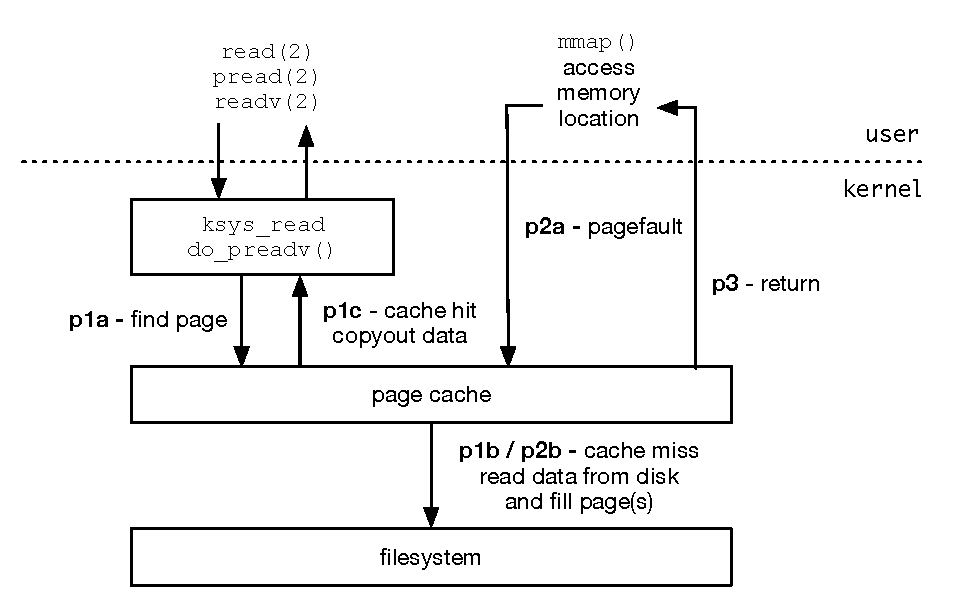
\includegraphics[scale=0.6]{figures/vfs-file-read}
	\centering
	\caption{The different ways that data is read from a file}
	\label{fig:vfs-read-file}
\end{figure}

\noindent
If the process enters the kernel through calling one of the read-related system calls (path p1a), the kernel will attempt to locate pages of cached data. For each page of data, if the page is resident (p1c) the kernel can simply copy the data from the cached page into the user-supplied buffer. If the page is not present (p1b), a call is made into the filesystem to read the data from disk into the page cache. From there, the data is copied to user-space (p1c) and the kernel returns with the amount of data read.

If the file had previously mapped the file and then accesses a location in memory that is covered by the mapping, it will get a page fault and enter the kernel (path p2a). The kernel validates the address and make a call into the filesystem (p2b) whereby data will be read from disk to fill the page. Once that is complete, the kernel returns to the process (p3) and the read is successfully made on the second attempt.

Note tll reads and writes go through the page cached unless a file is opened with \cf{O\_DIRECT} which will be covered in section \textbf{XXX -- TBD}.

\begin{table}[h]
\begin{tabular}{ll}
\parbox[l]{0.6in}{
\includegraphics[scale=0.8]{figures/src-xref.pdf}} & \parbox[l]{4in}{\small{The kernel read paths starts in \cf{fs/read\_write.c} and XXX}}
\end{tabular}
\end{table}

\noindent
First of all, the \cf{read(2)} system call enters the kernel as follows:

\begin{lstlisting}
SYSCALL_DEFINE3([*\bfseries read*], unsigned int, fd, 
                char __user *, buf, size_t, count)
{
    return [*\bfseries ksys\_read*](fd, buf, count);
}
\end{lstlisting}

\noindent
Tasks performed by \cf{ksys\_read()} are shown below and include using the file descriptor to locate the appropriate \cf{file} structure from which the current file offset can be found with a call to \cf{file\_ppos()}. The offset is stored in \cf{file->f\_pos}). 

\begin{lstlisting}
ssize_t 
[*\bfseries ksys\_read*](unsigned int fd, char __user *buf, size_t count)
{
    struct fd f = [*\bfseries fdget\_pos*](fd);
    ssize_t ret = -EBADF;

    if (f.file) {
        loff_t pos, *ppos = [*\bfseries file\_ppos(*]f.file);
        if (ppos) {
            pos = *ppos;
            ppos = &pos;
        }
        ret = [*\bfseries vfs\_read*](f.file, buf, count, ppos);
        if (ret >= 0 && ppos)
            f.file->f_pos = pos;
        [*\bfseries fdput\_pos*](f);
    }
    return ret;
}
\end{lstlisting}

\noindent
Once we have the file offset, a call is made to \cf{vfs\_read()} which first checks to see that the number of bytes to read and the file offset (and combination thereof) are valid values with a call to \cf{rw\_verify\_area()}. Next, the kernel checks to see which read function the underlying filesystem has exported and makes a call to it. Some filesystems provide their own \cf{read()} function and others utilize the generic \cf{generic\_file\_read\_iter()} function. \textbf{XXX -- need to say why at some point - it's all a bit of a mess. There is a .read function and a .read\_iter function. No FS seems to set .read other than for directories. Take BFS as an example, .read is set to generic\_read\_dir() and /read\_iter is set to generic\_file\_read\_iter().}

\begin{lstlisting}
ssize_t 
[*\bfseries vfs\_read*](struct file *file, char __user *buf, size_t count, 
         loff_t *pos)
{
    ssize_t ret;
        
    ret = [*\bfseries rw\_verify\_area*](READ, file, pos, count);
    
    if (file->f_op->read)
        ret = file->f_op->[*\bfseries read*](file, buf, count, pos);
    else if (file->f_op->read_iter) 
        ret = [*\bfseries new\_sync\_read*](file, buf, count, pos);
    else
        ret = -EINVAL;
    return ret;
}
\end{lstlisting}

\noindent
x

NOTE - read\_iter may have something to do with async i/o - \textit{possibly asynchronous read with iov\_iter as destination} - see https://lwn.net/Articles/535034/ for more information

SPFS doesn't set a "read" operation but it does set "generic\_file\_read\_iter" as the "read\_iter" function.

%%%%%%%%%%%%%%%%%%%%%%%%%%%%%%%%%%%%%%%%%%%%%%%%%%%%%%%%%%%%%%

\subsection{The \cf{new\_sync\_read()} and \cf{generic\_file\_read\_iter()} Functions}

x

\small
\bigskip 
\cf{vfs\_read()} $\rightarrow$ \cf{new\_sync\_read()}  $\rightarrow$ \cf{call\_read\_iter()}

\vspace{1pt}
\hspace{1.37in}$\rightarrow$ \cf{generic\_file\_read\_iter()} $\rightarrow$ \cf{filemap\_read()}
%\\~\\
    
\bigskip
\normalsize
\noindent


In \cf{filemap\_read()} data will be copied from the page cache into buffers in user-space.  If the data is not currently present, a combination(?) of the readahead and read\_folio address\_space operations are used to fetch it. Here is the code ...

\begin{lstlisting}
filemap_read()
    - loop around each iocb (one for regular read)
        - error = filemap_get_pages(iocb, iter->count, &fbatch, iov_iter_is_pipe(iter));
        - copied = copy_folio_to_iter(folio, offset, bytes, iter); calls following

copy_page_to_iter():
    - void *kaddr = kmap_local_page(page);
    - size_t n = min(bytes, (size_t)PAGE_SIZE - offset);
    - n = _copy_to_iter(kaddr + offset, n, i);
\end{lstlisting}

\noindent
Hmm! I can't see where the FS gets calls. Perhaps it just faults on the mapping above?

%------------------------------------------------------------------------------------------------------------------------------------------------------------------------

\subsection{Vectored Reads}

There are several entry points into the kernel for vectored reads. In the \cf{fs} directory:

\begin{lstlisting}
$ [*\bfseries grep SYSCALL *.c | grep readv*]
read_write.c:SYSCALL_DEFINE3([*\bfseries readv*], unsigned long, fd, ...
read_write.c:SYSCALL_DEFINE5([*\bfseries preadv*], unsigned long, fd, ...
read_write.c:SYSCALL_DEFINE6([*\bfseries preadv2*], unsigned long, fd, ...
read_write.c:COMPAT_SYSCALL_DEFINE4([*\bfseries preadv64*], ...
read_write.c:COMPAT_SYSCALL_DEFINE5([*\bfseries preadv*], ...
read_write.c:COMPAT_SYSCALL_DEFINE5([*\bfseries preadv64v2*], ...
read_write.c:COMPAT_SYSCALL_DEFINE6([*\bfseries preadv2*], ...
\end{lstlisting}

\noindent
XXX - Most functions end up calling \cf{do\_preadv()} which simply gets the \cf{file} structure associated with the file descriptor and then makes a call to \cf{vfs\_readv()}:

\begin{lstlisting}
static ssize_t 
[*\bfseries do\_preadv*](unsigned long fd, const struct iovec __user *vec,
             unsigned long vlen, loff_t pos, rwf_t flags)
{       
    struct fd f;
        
    f = fdget(fd);
    if (f.file) {
        ret = -ESPIPE;
        if (f.file->f_mode & FMODE_PREAD)
           ret = [*\bfseries vfs\_readv*](f.file, vec, vlen, &pos, flags);
        fdput(f);
    }
    return ret;
}
\end{lstlisting}

\noindent
xx

%%%%%%%%%%%%%%%%%%%%%%%%%%%%%%%%%%%%%%%%%%%%%%%%%%%%%%%%%%%%%%%

\section{Writing Files}

How data is written to disk depends on the flags that were passed to the \cf{open(2)} system call. The first part of this section will explore the general case where no flags are specified. This type of writing is called \textit{buffered I/O}. The basic set of operations to be performed in this case follow the general path as follows:

\textbf{I like the idea but need to really understand this before deciding whether or not to keep it.}

\begin{quote}
By default, kernel marks written pages dirty and flushes after a delay:
write(fd, ”hello world”, 11);
1. Kernel writes “hello world” to page for cached disk
2. Kernel adds the page to the “dirty list”—pages that have been modified but not yet written to disk
3. Periodically, kernel writes all pages in dirty list to disk
\end{quote}

\noindent
The \cf{write(2)} system call enters the kernel as follows (\cf{fs/read\_write.c}:

\begin{lstlisting}
SYSCALL_DEFINE3([*\bfseries write*], unsigned int, fd, 
                const char __user *, buf, size_t, count)
{
    return [*\bfseries ksys\_write*](fd, buf, count);
}
\end{lstlisting}

\noindent
x

\begin{lstlisting}
ssize_t 
[*\bfseries ksys\_write*](unsigned int fd, const char __user *buf, 
           size_t count)
{
    struct fd f = [*\bfseries fdget\_pos*](fd);
    ssize_t ret = -EBADF;

    if (f.file) {
        loff_t pos, *ppos = [*\bfseries file\_ppos*](f.file);
        if (ppos) {
            pos = *ppos;
            ppos = &pos;
        }
        ret = [*\bfseries vfs\_write*](f.file, buf, count, ppos);
        if (ret >= 0 && ppos)
            f.file->f_pos = pos;
        [*\bfseries fdput\_pos*](f);
    }

    return ret;
}
\end{lstlisting}

\noindent
x

%------------------------------------------------------------------------------------------------------------------------------------------------------------------------

\subsection{Vectored Writes}

TBD

%%%%%%%%%%%%%%%%%%%%%%%%%%%%%%%%%%%%%%%%%%%%%%%%%%%%%%%%%%%%%%%

\section{Direct I/O}\label{kernel-direct-io}

TBD

% https://www.oreilly.com/library/view/understanding-the-linux/0596005652/ch16s03.html

%%%%%%%%%%%%%%%%%%%%%%%%%%%%%%%%%%%%%%%%%%%%%%%%%%%%%%%%%%%%%%%

\section{File Locking Implementation}

TBD - advisory and mandatory locking

% https://www.kernel.org/doc/Documentation/filesystems/mandatory-locking.txt


%------------------------------------------------------------------------------------------------------------------------------------------------------------------------

\section{Dissecting The proc Filesystem}

The main features of the proc filesystem was described in section \ref{procfs}. This section describes some of the interfaces of the filesystem that are used by other parts of the kernel including other filesystems. 

\begin{table}[h]
\begin{tabular}{ll}
\parbox[l]{0.6in}{
\includegraphics[scale=0.8]{figures/src-xref.pdf}} & \parbox[l]{4in}{\small{Much of the proc filesystem code can be found under \cf{fs/proc}. The code for displaying the contents of \cf{/proc/filesystems} is in \cf{fs/filesystems.c}.}}
\end{tabular}
\end{table}

To demonstrate a part of procfs, consider the output displayed when looking at the list of available filesystems. There are over 30 entries on my Ubuntu 22.10 VM. Note the output shown here is available and not mounted filesystems.

\begin{lstlisting}
$ [*\bfseries cat /proc/filesystems*]
nodev   sysfs
nodev   tmpfs
nodev   bdev
nodev   proc
...
nodev   sockfs
...
nodev   devpts
        ext3
        ext2
        ext4
        squashfs
        vfat
nodev   ecryptfs
\end{lstlisting}

\noindent
There are two components to creating the \cf{filesystems} entry under \cf{/proc} and displaying the contents of the file. First, a call is made to create an entry in the namespace (\cf{fs/filesystems.c}). 

\begin{lstlisting}
static int __init proc_filesystems_init(void)
{
    [*\bfseries proc\_create\_single*]("filesystems", 0, NULL, 
                       filesystems_proc_show);
    return 0;
}
\end{lstlisting}

\noindent
Note that this is a macro and results in a call to \cf{proc\_create\_single\_data()}. In the same file the code to display the contents of the available filesystems is very simple. It simply walks through the list of available filesystems referenced by \cf{file\_systems}, displays each entry together with information about whether the filesystem requires a device or not. For example \cf{proc} is a pseudo filesystem so doesn't require a device but the \cf{ext*} filesystems do.

\begin{lstlisting}
static int filesystems_proc_show(struct seq_file *m, void *v)
{
    struct file_system_type * tmp;

    read_lock(&file_systems_lock);
    tmp = [*\bfseries file\_systems*];
    while (tmp) {
        seq_printf(m, "%s\t%s\n",
            (tmp->fs_flags & FS_REQUIRES_DEV) ? "" : "nodev",
            tmp->name);
        tmp = tmp->next;
    }
    read_unlock(&file_systems_lock);
    return 0;
}
\end{lstlisting}

\noindent
\cf{seq\_printf()} is used to display each entry in the file - calls multiple fns to handle arguments. Need to find last one?

A call to \cf{proc\_create\_single\_data()} differs from \cf{proc\_create\_single()} in that callers may wish to pass data that is stored in the \cf{data} field of the \cf{proc\_dir\_entry} structure that will be allocated for this node. The data passed will be available on a subsquent call - \textbf{XXX---where does this happen or do the callers extract is themselves somehow?}

The function to display the file contents is passed to \cf{proc\_create\_single()} and is stored .... XXX

Note that you can pass more than a single name to \cf{proc\_create\_single\_data()} as some modules do:

\begin{lstlisting}
proc_create_single_data("driver/atmel", ...
proc_create_single_data("driver/rtc"
\end{lstlisting}

% proc_create and proc_remove??? - https://devarea.com/linux-kernel-development-creating-a-proc-file-and-interfacing-with-user-space/#.Y9foYS-B1p8

% create_proc_entry vs remove_proc_entry - https://linux.die.net/lkmpg/x769.html

\subsection{Use of Red-Black Trees in /proc}

The proc filesystem tree is stored in memory as a \textit{red-black tree} (\cf{struct rb\_node}). Red-black trees are a type of self-balancing binary tree, and are used by several places in the kernel for storing sortable key/value data pairs. Each node node in the tree has a bit representing \textit{color} (red or black) which is used to ensure that the tree remains balanced during insertion and delete operations.

You can read the background and details about the Linux red-black tree implementation in \cf{Documentation/rbtree.txt}.

% https://www.kernel.org/doc/Documentation/rbtree.txt

The root of the proc tree is accessed by \cf{proc\_root}. Some of the fields are shown below. The operations for this root node are very simple in terms of returning attributes and providing a \textit{lookup} function so that directories and files under \cf{/proc} can be located and displayed.


\begin{lstlisting}
struct proc_dir_entry proc_root = {
  proc_iops = 0xffff8000092be640 <proc_root_inode_operations>,
  {
    proc_ops = 0xffff8000092be700 <proc_root_operations>,
    proc_dir_ops = 0xffff8000092be700 <proc_root_operations>
    ....
    name = 0xffff80000984c208 "/proc",
  },

  subdir = {
    rb_node = 0xffff0000c01bc808
  },

struct inode_operations proc_root_inode_operations = {
    .lookup     = proc_root_lookup,
    .getattr    = proc_root_getattr,
}
\end{lstlisting}

\noindent
Nodes are added to the tree during system initialization or when kernel modules are loaded.

\subsection{KGDB --- Analyzing the \cf{/proc} File Tree}

Lookup walks through the rb\_left / rb\_right links recursively until if finds the node

There is a gdb command \cf{lx\_rb\_first} / function that can help - see apropos lx. there are several of them.

\begin{lstlisting}
crash> p proc_root | grep rb_node
    rb_node = 0xffff5a09c01ba208
crash> tree -t rbtree -o proc_dir_entry.subdir -N 0xffff5a09c01ba208
ffff5a09c01ba188
ffff5a09c01ba488
ffff5a09c01ba008
ffff5a09c01ba248
ffff5a09c0422308
ffff5a09c01baa88
ffff5a09c05190c8
ffff5a09c0422788
ffff5a09c01bad88
ffff5a09c01ba908
...
\end{lstlisting}

%%%%%%%%%%%%%%%%%%%%%%%%%%%%%%%%%%%%%%%%%%%%%%%%%%%%%%%%%%%%%%%

\section{Quotas Implementation}

TBD

%%%%%%%%%%%%%%%%%%%%%%%%%%%%%%%%%%%%%%%%%%%%%%%%%%%%%%%%%%%%%%%

\section{Handling Pipes}\label{vfs-pipes}

TBD

%%%%%%%%%%%%%%%%%%%%%%%%%%%%%%%%%%%%%%%%%%%%%%%%%%%%%%%%%%%%%%%

\section{Flushing File Data and Metadata}\label{vfs-sync}

TBD - no other place that covers this?


%%%%%%%%%%%%%%%%%%%%%%%%%%%%%%%%%%%%%%%%%%%%%%%%%%%%%%%%%%%%%%%

\section{Filesystem Interfaces}\label{vfs-operations}

This section is a reference to the operations that filesystems can support through the following interfaces:

\begin{itemize}
	\item \cf{super\_operations}
	\item \cf{inode\_operations}
	\item \cf{file\_operations}
	\item \cf{address\_space\_operations}

\end{itemize}

\noindent
It is unlikely that each filesystem will support all of the operations for each of these structures. What is supported generally depends on the features that the filesystem supports in addition to how much control over file operations it requires. For example, some filesystems will have simpler implementations and therefore include generic kernel functions for some aspects.

It isn't necessary to read everything in this section as there is a lot of detail and understanding all interfaces isn't necessary to understanding the basics of filesystem operations. But to go into detail, knowledge of more of these interfaces is necessary so they're all listed here.

%----------------------------------------------------------------------------------------------------------------------------------------------------------

\subsection{The \cf{super\_operations} Structure}

The \cf{super\_operations} structure contains operations that operate on the filesystem as opposed to individual files. Filesystems attach their \cf{super\_operations} structure to the \cf{s\_op} field of the \cf{super\_block} structure during a call to their \cf{fill\_super()} function. For SPFS, the flow is shown in figure \ref{fig:super-operations} from a call to \cf{module\_init()} when the module is loaded followed by a call into SPFS (via \cf{sp\_mount()} each time an SPFS filesystem is mounted.

There are a lot of \cf{super\_operations} of which many functions are not implemented by each filesystem. For example, out of the 29 possible functions. 3 of the functions are only used if \cf{CONFIG\_QUOTA} is defined. SPFS only implements 6 of these functions.

Below we give a brief description of each function:

\begin{itemize}
    \item \cf{alloc\_inode} -- his method is called by alloc\_inode() to allocate memory for struct inode and 
    		initialize it.  If this function is not defined, a simple 'struct inode' is allocated.  Normally 
		alloc\_inode will be used to allocate a larger structure which contains a 'struct inode' embedded within it.
    \item \cf{destroy\_inode} --
    \item \cf{free\_inode} -- 
    \item \cf{dirty\_inode} -- 
    \item \cf{write\_inode} -- called when the kernel needs to write an inode to disk. An example would be for file 
    	creation. A new file is created and the inode is marked dirty. The same is true for the inode of the parent 
	directory. The filesystem calls \cf{mark\_inode\_dirty()} for both inodes. The second parameter specifies 
	whether the write should be synchronous or not but not all filesystems check this flag.
    \item \cf{drop\_inode} -- 
    \item \cf{evict\_inode} -- this should only be called when both the inode's \cf{i\_nlink} and \cf{i\_count} 
    	both go to zero. When a file has been removed but may still be referenced by processes, it can't be 
	deleted until the last reference goes away. When this happens, the \cf{evict\_inode} operation is called.
    \item \cf{put\_super} -- called as part of \cf{umount} before the \cf{super\_block} will be freed.
    \item \cf{sync\_fs} --
\end{itemize}    

\noindent

%%%%%%%%%%%%%%%%%%%%%%%%%%%%%%%%%%%%%%%%%%%%%%%%%%%%%%%%%%%%%%%

\subsubsection{Freeze/Thaw Functions}\label{freeze}

The only filesystem to provide support for these operations is gfs2.
    
\begin{itemize}
    \item \cf{freeze\_super} --
    \item \cf{freeze\_fs} --
    \item \cf{thaw\_super} --
    \item \cf{unfreeze\_fs} --
\end{itemize}    

%%%%%%%%%%%%%%%%%%%%%%%%%%%%%%%%%%%%%%%%%%%%%%%%%%%%%%%%%%%%%%%

\subsubsection{Information Gathering Functions}

\begin{itemize}    
    \item \cf{statfs} -- called in response to\cf{df(1)} and \cf{stat -f} commands. See \cf{fs/statfs.c} for kernel routines
    	that handle filesystem statistics. \textbf{XXX---need some sort of trace to figure out which of the many functions
	is called. There are several.}    \item \cf{remount\_fs} --
    \item \cf{umount\_begin} --
    \item \cf{show\_options} --
    \item \cf{show\_devname} --
    \item \cf{show\_stats} -- if a filesystem supports this function, it is called by the proc filesystem (see \cf{proc\_namespace.c})
    	when doing \textbf{XXX}
    \item \cf{show\_path} -- as above, this function is called by the proc filesystem (\cf{show\_mountinfo()}) - XXX seems
    	to do very little other than add tabs and stuff. Weird.
    \item \cf{nr\_cached\_objects} --
    \item \cf{free\_cached\_objects} --
\end{itemize}

%%%%%%%%%%%%%%%%%%%%%%%%%%%%%%%%%%%%%%%%%%%%%%%%%%%%%%%%%%%%%%%

\subsubsection{Qutoas-related Functions}
    
\begin{itemize}
    \item \cf{quota\_read} --
    \item \cf{quota\_write} --
    \item \cf{get\_dquots} --
\end{itemize}

\noindent
TBD

%%%%%%%%%%%%%%%%%%%%%%%%%%%%%%%%%%%%%%%%%%%%%%%%%%%%%%%%%%%%%%%

\subsection{The \cf{inode\_operations} Structure}

The \cf{inode\_operations} is accessed from the \cf{i\_iop} field of the Linux \cf{inode} structure. It is set by the filesystem when new files are created or files are read from disk. This allows the kernel to call into the filesystem for a specific inode.

Several of these options take a \cf{user\_namespace} structure as an argument \textbf{XXX---how is it used?}

\begin{itemize}
    \item \cf{readlink} -- 
    \item \cf{create} -- 
    \item \cf{link} -- 
    \item \cf{unlink} -- 
    \item \cf{symlink} -- 
    \item \cf{mkdir} -- create a directory. The parent inode is passed together with the file mode and a negative dentry for the 
    	new directory entry. If the call is successful, the filesystem will call \cf{d\_instantiate()} to XXX the new file. XXX need right 
	words here.
    \item \cf{rmdir} -- remove a directory. The parent inode is passed together with the dentry for the file to be removed. XXX who
    	"deletes" the dentry? Look at the kernel source.
    \item \cf{mknod} -- 
    \item \cf{rename} -- 
    \item \cf{setattr} -- 
    \item \cf{getattr} -- 
    \item \cf{listxattr} -- 
    \item \cf{fiemap} -- 
    \item \cf{update\_time} -- 
    \item \cf{atomic\_open} -- 
    \item \cf{tmpfile} -- 
    \item \cf{set\_acl} -- 
    \item \cf{fileattr\_set} -- 
    \item \cf{fileattr\_get} -- 
\end{itemize}

\noindent
XXX

%%%%%%%%%%%%%%%%%%%%%%%%%%%%%%%%%%%%%%%%%%%%%%%%%%%%%%%%%%%%%%%

\subsection{The \cf{file\_operations} Structure}

Functions that apply to regular files are held in the \cf{file\_operations} (\textbf{XXX---except i have one for dirops which has a few functions in it. Need to explain}

A pointer to this structures is attached to the \cf{f\_op} field of the inode structure.

Filesystems typically define two \cf{file\_operations} structures - or do they?

\begin{itemize}
    \item \cf{llseek} -- ext4 dir lseek / XFS does something with holes. 
    \item \cf{read} -- XXX - Many filesystems don't provide this function and instead, have all I/O go through the page cache
    	which utilizes the \cf{address\_space\_operations} structure. procfs and others for which page cache I/O make no sense.
	There are a lot of them that provide this so need to look.
    \item \cf{write} -- XXX - Many filesystems don't provide this function and instead, have all I/O go through the page cache
    	which utilizes the \cf{address\_space\_operations} structure.
    \item \cf{read\_iter} --
    \item \cf{write\_iter} --
    \item \cf{iopoll} --
    \item \cf{iterate} --
    \item \cf{iterate\_shared} --
    \item \cf{poll} --
    \item \cf{unlocked\_ioctl} --
    \item \cf{compat\_ioctl} --
    \item \cf{mmap} --
    \item \cf{open} --
    \item \cf{flush} --
    \item \cf{release} --
    \item \cf{fsync} --
    \item \cf{fasync} --
    \item \cf{lock} --
    \item \cf{sendpage} --
    \item \cf{get\_unmapped\_area} --
    \item \cf{check\_flags} --
    \item \cf{flock} --
    \item \cf{splice\_read} --
    \item \cf{splice\_write} --
    \item \cf{setlease} --
    \item \cf{fallocate} --
    \item \cf{show\_fdinfo} --
    \item \cf{mmap\_capabilities} --
    \item \cf{copy\_file\_range} --
    \item \cf{remap\_file\_range} --
    \item \cf{fadvise} --
    \item \cf{uring\_cmd} --
    \item \cf{uring\_cmd\_iopoll)} -- xx
\end{itemize}

\noindent
xxx

%%%%%%%%%%%%%%%%%%%%%%%%%%%%%%%%%%%%%%%%%%%%%%%%%%%%%%%%%%%%%%%

\subsection{The \cf{address\_space\_operations} Structure}

page cache doc - http://sylab-srv.cs.fiu.edu/lib/exe/fetch.php?media=paperclub:lkd3ch16.pdf 

Folios - https://lwn.net/Articles/869942/
% https://www.phoronix.com/search/folios

%%%%%%%%%%%%%%%%%%%%%%%%%%%%%%%%%%%%%%%%%%%%%%%%%%%%%%%%%%%%%%%

\subsubsection{Memory Folio Functions}

Section \ref{memory-folios} described changes in Linux kernel memory management for supporting \textit{memory folios}, a mechanism that allow filesystems and the page cache to manage memory in larger chunks than \cf{PAGE\_SIZE} which can, depending on the workload, give a performance enhancement of 0-10\%.

The functions that filesystems provide for supporting memory folios, utilize the \cf{folio} structure which is defined in \cf{include/linux/mm\_types.h} as:

\begin{lstlisting}
struct folio {
    union {
        struct {
            unsigned long flags;
            union {
                struct list_head lru;
                struct { 
                    void *__filler;
                    unsigned int mlock_count;
                };
            };
            struct address_space *mapping;
            pgoff_t index;
            void *private;
            atomic_t _mapcount;
            atomic_t _refcount;
            unsigned long memcg_data; 
        };
        struct page page;
    };
};
\end{lstlisting}

\noindent
Here are the interfaces into the filesystem for supporting memory folios.

\begin{itemize}
    \item \cf{read\_folio} -- read XXX looks like this replaced the old \cf{readpage()} function.
    \item \cf{dirty\_folio} --
    \item \cf{invalidate\_folio} --
    \item \cf{release\_folio} --
    \item \cf{launder\_folio} --
    \item \cf{free\_folio} --
\end{itemize}

\noindent
XXX check which filesystems do interesting things.

SPFS, which will be introduced in the next chapter, represents the simplest case of filesystem folio support. It simply relies on kernel support functions for handling folios:

\begin{lstlisting}
struct address_space_operations sp_aops = {
    .dirty_folio        = [*\bfseries block\_dirty\_folio*],
    .invalidate_folio   = [*\bfseries block\_invalidate\_folio*],
    .read_folio         = [*\bfseries sp\_read\_folio*],
    .writepage          = sp_writepage,
    .write_begin        = sp_write_begin,
    .write_end          = sp_write_end,
    .bmap               = sp_bmap
};
\end{lstlisting}

\noindent
with \cf{sp\_read\_folio} being a simple function calling \cf{block\_read\_full\_folio()} passing \cf{sp\_get\_block()} so that the kernel can get block numbers for specific portions of the file covered by the folio.

\begin{lstlisting}
int
sp_read_folio(struct file *file, struct folio *folio)
{
    return block_read_full_folio(folio, sp_get_block);
}
\end{lstlisting}

\noindent
Other filesystems have more complicated implementations. XXX will be described at some point.

%%%%%%%%%%%%%%%%%%%%%%%%%%%%%%%%%%%%%%%%%%%%%%%%%%%%%%%%%%%%%%%

\subsubsection{Blah blah Functions}

\begin{itemize}
    \item \cf{writepage} --
    \item \cf{writepages} --
    \item \cf{readahead} --
    \item \cf{write\_begin} --
    \item \cf{write\_end} --
    \item \cf{bmap} --
    \item \cf{direct\_IO} --
    \item \cf{migratepage} --
    \item \cf{isolate\_page} --
    \item \cf{putback\_page} --
    \item \cf{is\_partially\_uptodate} --
    \item \cf{is\_dirty\_writeback} --
    \item \cf{error\_remove\_page} --
\end{itemize}

\subsubsection{Swapping Functions}

\begin{itemize}
    \item \cf{swap\_activate} --
    \item \cf{swap\_deactivate} --
    \item \cf{swap\_rw} --
\end{itemize}

\noindent
XXX

%%%%%%%%%%%%%%%%%%%%%%%%%%%%%%%%%%%%%%%%%%%%%%%%%%%%%%%%%%%%%%%

\section{Conclusion}

This chapter continued to build on the previous chapter which described the main kernel structures, by describing in detail, the kernel functions in the Linux VFS layer that deal with filesystem access. There has been a lot of material presented here together with a lot of examples of using \cf{gdb} to help analyze the paths through the kernel. It's not an east subject to study and there is limited documentation online. There are a few, detailed examples, particularly in the area of pathname resolution, XXX and YYY. The goal of this chapter is to pull those areas of information together with areas that are not well documented and give you the tools to explore each area in more detail.

Setting up \cf{gdb} / \cf{kgdb} is often a challenge. For my Macbook Pro with Apple's m1 CPU, I spent the better part of six months trying to find answers about how to get breakpoints working. At the time of writing, my only option was to emulate x86\_64 VMs which resulted in a kernel compilation that was about 17 times longer than compiling for the native CPU. But it's a task that I think is well worth the effort. Setting breakpoints and walking through the kernel code is the best way to understand what is happening.

The next chapter will help with putting the pieces together by showing how to implement a simple, disk-based filesystem and use debugging tools to help better understand the flow through the kernel into the filesystem in response to various system calls.


